\documentclass[12pt,a4paper]{article}

% ── 中文支持 ─────────────────────────────────────────────────
\usepackage{xeCJK}
\xeCJKsetup{CJKspace=true}
\setCJKmainfont{Noto Serif CJK SC}[AutoFakeBold=true, AutoFakeSlant=true]
\setCJKsansfont{Noto Sans CJK SC}
\setCJKmonofont{Noto Sans Mono CJK SC}
\setCJKfamilyfont{song}{Noto Serif CJK SC}
\setCJKfamilyfont{kai}{Noto Serif CJK SC}

% ── 数学 ─────────────────────────────────────────────────────
\usepackage{amsmath,amssymb,amsthm,mathtools}
\numberwithin{equation}{section}
\DeclareMathOperator*{\argmax}{argmax}

% ── 图表 ─────────────────────────────────────────────────────
\usepackage{booktabs}
\usepackage{graphicx}
\graphicspath{{data/figures/}}
\usepackage{float}
\usepackage[font=small,skip=5pt]{caption}
\usepackage{subcaption}
\usepackage{array}
\usepackage{longtable}
\usepackage{multirow}

% ── 参考文献 ─────────────────────────────────────────────────

% ── 超链接 ───────────────────────────────────────────────────
\usepackage{hyperref}
\hypersetup{
  colorlinks=true,
  linkcolor=blue!60!black,
  citecolor=blue!60!black,
  urlcolor=blue!60!black,
  unicode=true,
  hidelinks=false
}

% ── 版面 ─────────────────────────────────────────────────────
\usepackage{geometry}
\geometry{
  a4paper,
  top=2.5cm, bottom=2.5cm,
  left=3.0cm, right=2.5cm
}
\usepackage{indentfirst}
\usepackage{setspace}
\setstretch{1.5}
% 五号=12pt，首行缩进2字（约1.95em），段间距
\setlength{\parindent}{1.98em}
\setlength{\parskip}{0pt}
\setlength\textfloatsep{8pt}
\setlength\abovecaptionskip{3pt}
\setlength\belowcaptionskip{6pt}

% ── 标题格式（分级编号）────────────────────────────────────────
\usepackage{titlesec}
% 第一级：1 2 3，小四号黑体（14pt bold），段前后0.5行
\titleformat{\section}{\CJKfamily{kai}\bfseries\fontsize{14}{20}\selectfont}{\thesection}{0.5em}{}
\titlespacing*{\section}{0pt}{0.5em}{0.5em}
% 第二级：2.1 2.2，五号字体
\titleformat{\subsection}{\CJKfamily{kai}\bfseries\fontsize{12}{17}\selectfont}{\thesubsection}{0.4em}{}
\titlespacing*{\subsection}{0pt}{0.4em}{0.4em}
% 第三级：2.2.1，五号字体
\titleformat{\subsubsection}{\CJKfamily{kai}\bfseries\fontsize{12}{17}\selectfont}{\thesubsubsection}{0.3em}{}
\titlespacing*{\subsubsection}{0pt}{0.3em}{0.3em}

% ── 页面样式 ─────────────────────────────────────────────────
\usepackage{fancyhdr}
\pagestyle{plain}
\fancyhf{}\fancyfoot[C]{\thepage}
\pagestyle{fancy}

% ─────────────────────────────────────────────────────────────
\begin{document}

% ── 标题块（中文）─────────────────────────────────────────────
\begin{center}
  \vspace*{0.5cm}
  {\CJKfamily{kai}\bfseries\fontsize{14}{20}\selectfont 体裁、朝代与语义空间：中国古典诗歌的计算测量与稳健性检验\par}
  \vspace{0.5em}
  {\fontsize{11}{16}\selectfont\itshape Genre, Dynasty, and Semantic Space: Computational Measurement and Robustness Checks in Classical Chinese Poetry\par}
  \vspace{0.8em}

  % 中文摘要
  {\CJKfamily{kai}\bfseries\fontsize{14}{20}\selectfont 摘\quad 要\par}
  \vspace{0.4em}
  \parbox{0.92\linewidth}{\fontsize{10.5}{14}\selectfont%
    本研究基于111万余首中国古典诗歌，为4,634位诗人构建BERT-CCPoem语义嵌入，运用PCoA--PERMANOVA、PCA、Louvain社区检测进行多重稳健性检验。核心发现：（1）PCoA--PERMANOVA双因素分解显示，朝代条件$R^{2}=0.203$（$F=222.78$），体裁条件$R^{2}=0.075$（$F=246.80$），二者在三种合法置换方案下均$p\leq0.001$——语义空间呈现\textbf{"朝代主导全局、体裁形成独立分化"}的双层结构。（2）词（ci）诗人构成极强的局部内聚社区：ci--ci互文距离0.762，比非词诗人（0.969）小21\%，Cohen's $d=1.90$；诗人级block bootstrap给出距离差0.207（95\% CI $[0.189,0.225]$），$d$的95\% CI $[1.54,2.20]$，不依赖诗人对伪重复。（3）Louvain体裁纯度净增0.021（$p<0.001$），词派跨七朝构成语义共同体。（4）Label leakage三档对照实验确认，体裁可分性在剥离全部元数据、统一繁简正字法并去标点后依然稳健（宋诗vs宋词Accuracy=0.960，基线0.500），体裁信号源于词汇—语义内容。（5）语义引力非单调，排除了简单时间衰减模型。上述发现均锚定于BERT-CCPoem嵌入空间，跨模型推广需独立验证。本研究将文化记忆理论、体裁规范理论和多元系统论操作化为可量化分析框架，提出"\textbf{朝代地形}+\textbf{体裁分化}"双层结构以理解中国文学传统的内部组织。\par}
  \vspace{0.5em}

  % 中文关键词
  {\CJKfamily{kai}\bfseries\fontsize{10.5}{14}\selectfont 关键词：}\fontsize{10.5}{14}\selectfont BERT嵌入；中国古典诗歌；语义空间；体裁效应；PERMANOVA；文化记忆；词派；数字人文
  \vspace{0.8em}

\end{center}
\newpage
% ── 英文摘要 ──
\begin{center}
  {\bfseries\fontsize{14}{20}\selectfont ABSTRACT\par}
  \vspace{0.4em}
  \parbox{0.92\linewidth}{\fontsize{10.5}{14}\selectfont%
    This study investigates the semantic organization of classical Chinese poetry using 1.1 million poems and 4,634 poet embeddings generated by BERT-CCPoem. Through PCoA--PERMANOVA, PCA, and Louvain community detection, we find that dynasty and genre form a two-tier structure: dynasty dominates the global semantic topography, while genre carves out a smaller but independent secondary differentiation. Key findings: (1) PCoA--PERMANOVA two-factor decomposition yields dynasty conditional $R^{2}=0.203$ ($F=222.78$, $p\leq0.001$) and genre conditional $R^{2}=0.075$ ($F=246.80$, $p\leq0.001$), both significant under three permutation schemes. (2) Ci (song lyric) poets constitute the most cohesive local subspace: ci--ci intertextual distance is 0.762, 21\% smaller than non-ci poets (0.969), Cohen's $d=1.90$; poet-level block bootstrap yields a mean difference of 0.207 (95\% CI $[0.189,0.225]$) and a $d$ CI of $[1.54,2.20]$, confirming robustness against pseudo-replication. (3) Louvain genre purity shows a net increment of 0.021 ($p<0.001$); ci communities span seven dynasties. (4) A three-tier label-leakage control experiment confirms that genre separability survives metadata removal, orthography normalization, and punctuation stripping (within-Song shi vs.\ ci accuracy = 0.960, baseline 0.500), indicating lexical--semantic rather than format-driven differentiation. (5) Semantic gravity is non-monotonic, ruling out a simple temporal-decay model. All findings are specific to the BERT-CCPoem embedding space. We integrate cultural memory theory, genre convention theory, and polysystem theory to operationalize this ``dynastic topography + genre differentiation'' framework for understanding the internal organization of the Chinese poetic tradition.\par}
  \vspace{0.5em}

  % 英文关键词
  {\bfseries\fontsize{10.5}{14}\selectfont KEY WORDS:}\fontsize{10.5}{14}\selectfont BERT Embeddings; Classical Chinese Poetry; Semantic Space; Genre Effect; PERMANOVA; Cultural Memory; Ci School; Digital Humanities
\end{center}

\vspace{0.5cm}

\newpage

% ── 正文 ─────────────────────────────────────────────────────
\noindent

% ═══════════════════════════════════════════════════════════
\section{引言}
% ═══════════════════════════════════════════════════════════

\subsection{研究背景：中国古典诗歌研究的数字人文转向}

中国古典诗歌研究有着悠久的学术传统，长期以来以文本细读、版本校勘和作家作品考据为核心方法论。20世纪中叶以来，量化文学研究（quantitative literary studies）开始尝试以统计方法揭示文学史的宏观规律，但受制于手工编码的工作量瓶颈，这些探索始终未能规模化。近年来，自然语言处理技术的突破——尤其是预训练语言模型（pre-trained language models）的兴起——使得大规模语义表示学习成为可能，为文学研究开辟了新的路径。

BERT（Bidirectional Encoder Representations from Transformers, Devlin et al., 2019）作为近年来最具影响力的预训练模型，能够将文本映射为稠密的向量空间，使本文得以在语义层面比较任意文本对之间的相似性。中国古典诗歌领域也已出现多个大规模标注语料库（Zhou et al., 2021），为计算诗学（computational poetics）研究奠定了坚实的数据基础。

然而，既有计算诗学研究的关注点主要集中在诗歌生成（Li et al., 2020）、作者考证和主题建模等方面，对于中国古典诗歌语义空间的\textbf{内在几何结构}——即哪些因素组织了诗歌之间的语义关系、这些因素的相对贡献有多大、不同文学史因素如何在语义空间中几何化——尚缺乏系统性的实证研究。

\subsection{核心研究问题}

本研究旨在回答以下核心问题：\textbf{体裁形式与朝代分期，何者是组织中国古典诗歌语义空间的主导因素？}

这一核心问题可以分解为以下子问题：

\begin{itemize}
  \item \textbf{R1（效应量比较）}：体裁形式（ci/shi/qu）与朝代分期，何者解释了更多的语义距离方差？效应量差距有多大？
  \item \textbf{R2（社区结构）}：哪些文学形式在语义空间中形成了跨朝代的语义社区？体裁规范是否足以在语义空间中产生可检测的社区边界？
  \item \textbf{R3（维度结构）}：语义空间的主要变异维度是什么？这些维度更多承载体裁分化、还是历史分期、抑或二者复合的信号？
  \item \textbf{R4（形式约束的机制）}：体裁是否构成独立于朝代的组织因素？其机制是什么？词牌、诗格等形式约束是否足以解释ci体裁的语义内聚性？
\end{itemize}

\subsection{研究贡献}

本研究的主要贡献有四点：

\textbf{第一}，本研究通过PCoA--PERMANOVA双因素方差分解（McArdle--Anderson 2001框架），在大规模语料中定量揭示：朝代解释了较大的全局语义方差（条件$R^{2}=0.203$，$F=222.78$，$p\leq0.001$），体裁解释了较小但同样显著的独立方差（条件$R^{2}=0.075$，$F=246.80$，$p\leq0.001$）。在sequential、restricted within-stratum与Freedman--Lane三种合法置换方案下，朝代与体裁的条件效应均极显著且方向一致——这表明二者是两个独立但量级不同的组织因子，体裁并非朝代分布的简单代理。PERMDISP表明朝代散布差异较大（2.51$\times$），其较大$R^{2}$部分混合了组内散布与组间位置；体裁组内散布差异不显著（1.72$\times$），体裁效应更接近"组间位置差异"。需要强调：上述为观测数据的统计关联模式，不推断文学史上的因果发生顺序。

\textbf{第二}，本研究揭示了ci体裁的真实内聚效应。Cohen's $d=1.90$，为全项目最大效应量——ci--ci诗人对（平均距离0.762）比nonci--nonci诗人对（0.969）近21\%。Louvain社区检测显示体裁纯度（0.956）相对随机期望（0.935）的净增量为0.021（统计显著但量级微小，$p<0.001$），朝代纯度（0.535）与随机期望无显著差异；需结合PCoA--PERMANOVA中朝代主导全局方差、体裁保留独立贡献这一双层结构综合解读。词派跨七朝构成语义共同体，清代ci\_heavy 8人组内距离仅0.037，为体裁内聚提供了互补的强效应量证据。这一发现直接挑战了以朝代为框架的文学史叙事。

\textbf{第三}，本研究通过PCA三轴结构和线性探测验证（PC1-4联合对ci/shi分类准确率达86.8\%），为"体裁信号在低维投影中可识别"提供了降维几何证据——PC1是体裁与朝代复合载荷的复合轴，体裁信号在 PCA 中可被分类器读出，但其相对量级与朝代信号需要通过 PCoA-PERMANOVA 条件分解来定量比较。

\textbf{第四}，本研究将文化记忆理论（Assmann, 2011）、体裁规范理论（Frow, 2015; Devitt, 2004）和多元系统论（Even-Zohar, 1990）三条成熟理论路线在中国古典诗歌领域做操作化计算验证，提出形式约束（词牌/诗格）创造了语义内聚效应，并揭示了”语义引力”现象的非单调性——ci/qu诗人因创造独立语义子空间而暂时脱离唐诗引力场，为理解中国文学传统的内部结构提供了一个形式约束视角的理论框架。

\textbf{方法论范式说明}：本研究转向 PERMANOVA+PCA+Louvain 的语义空间分析框架，该框架保留了语义相似性的非树状几何结构。所有核心发现验证了\textbf{层级结构假设（HH）}的修正形式：在BERT-CCPoem语义空间中，朝代构成主要的全局组织因素（条件$R^{2}=0.203$），体裁形成独立的局部次级分化（条件$R^{2}=0.075$）；ci体裁表现出极强的局部内聚性（Cohen's $d=1.90$），能够在朝代主导的语义地形之上创造一个更紧致的语义子空间。

\subsection{论文结构}

本文结构如下：第2节综述计算文学研究、BERT嵌入、文化记忆理论与体裁研究的相关文献；第3节介绍数据来源、诗人嵌入模型和元数据集成；第4节详述研究方法；第5节报告核心实证结果；第6节进行理论讨论；第7节总结全文并指出未来方向。

% ═══════════════════════════════════════════════════════════
\section{文献综述}
% ═══════════════════════════════════════════════════════════

\subsection{远读范式与计算文学研究的兴起}

传统文学研究以“近读”（close reading）为核心方法论，关注单篇文本的深度细读。然而，面对文学史上数以万计的文本累积，近读范式难以揭示宏观文学史的结构规律。Franco Moretti（2013）在《Distant Reading》中提出这一概念，主张以大规模量化方法处理文学文本，通过统计模式而非文本细节来理解文学史的演化轨迹。远读范式将文学视为一个由文本、作者、流派和传统构成的复杂系统，运用网络分析、谱系建模和量化风格分析等方法，揭示近读无法感知的宏观结构。

远读范式催生了一系列方法论工具。Underwood（2017, \textit{Digital Humanities Quarterly} 11(2)）系统梳理了远读范式的认识论基础，指出量化文学研究需要建立“测量与对象”之间的对应关系，存在“测量与对象不匹配”的风险。马晓（2026, 《宁夏大学学报》）则从算法批评的角度提出，当代计算文学实践需要直面“算法黑箱”与“人文解释”之间的张力，量化方法应与质性文学史研究形成对话。

\subsection{BERT语义嵌入与量化诗学研究}

预训练语言模型的发展使语义表示学习取得了突破性进展。BERT（Devlin et al., 2019, \textit{NAACL}）通过大规模无标注语料的预训练，在句级语义表示方面显著优于传统词袋模型和词嵌入方法——它能够将任意文本映射为高维稠密向量，使本文得以在语义空间中精确比较任意文本对之间的相似性。

在古典汉语处理领域，针对古典文献微调的专用BERT模型已形成系列：\textbf{BERT-CCPoem}（THUNLP-AIPoet团队）在926,024首中国古典诗歌语料（CCPC-Full v1.0）上预训练，采用512维隐层向量，是目前规模最大的中国古典诗歌语义表示模型；\textbf{GuwenBERT}（Huang et al., 2022）专注于文言文的语义表示\footnote{GuwenBERT: \url{https://github.com/ethan-yt/guwenbert}}；\textbf{SikuGPT}（Chang Liu et al., 2024, \textit{J. Comput. Cult. Herit.}）以四库全书语料训练，支持古籍智能信息处理。

BERT嵌入在诗歌研究中的应用可分为三类：\textbf{诗歌分类与风格判定}——Wang et al.（2022, arXiv）基于预训练模型实现古诗风格判定；\textbf{诗歌生成}——Hu \& Sun（2020, LREC）提出统一框架生成多种中国古典诗歌体裁；\textbf{情感分析}——Li et al.（2021, arXiv）构建CCPM诗歌匹配数据集，Gong \& Zhou（2025, arXiv）分析唐宋诗歌情感的历时演化。

\textbf{语义漂移}（semantic drift）是本研究的方法论近邻：Giulianelli et al.（2020, \textit{ACL}）利用BERT分析词汇的历时语义变化；Haider \& Eger（2019, arXiv）追踪德语诗歌中的语义变化和新意象。

\textbf{然而}，上述研究均将BERT嵌入作为下游任务（分类、生成）的特征输入，尚未有研究将语义空间自身的几何结构——即“哪些因素组织了诗人之间的语义关系”——作为研究对象。本研究正是对这一空白的直接填补。

\subsection{PERMANOVA与方差分解在文学研究中的应用}

方差分解方法回答一个根本问题：文学文本之间的语义差异，由哪些因素各自解释了多少？置换多元方差分析（PERMANOVA）由Anderson（2001, \textit{Austral Ecology}）提出，是处理距离矩阵的经典非参数方法，无需假设多元正态分布，适用于高维嵌入向量所生成的距离矩阵。Burns et al.（2021, \textit{NAACL}）利用词嵌入分析拉丁文学的互文性，验证了PERMANOVA对文学距离矩阵的有效性。然而，PERMANOVA在中国古典诗歌领域的应用尚属空白。本研究率先将PERMANOVA应用于中国古典诗歌语义空间的方差分解。

\subsection{Louvain社区检测与文学流派识别}

社区检测是网络科学的核心方法之一，用于识别图中联系紧密的节点群体。Louvain算法（Blondel et al., 2008, \textit{J. Statistical Mechanics}）通过优化模块度，在大规模网络上高效识别高质量社区。Hamilton \& S\o rensen（2026, \textit{Digital Scholarship in the Humanities}）将Louvain与HDBSCAN结合，提出“共识社区”方法，发现文本可“独立于传统文学分类”自组织为语义社区。

对于中国古典诗歌，社区检测具有特殊价值：文学流派（如“山水诗派”、“词派”）的边界往往是模糊的、历史学者争议颇大的。社区检测提供了一种数据驱动的流派边界识别方法，使本文得以超越主观归类，基于客观的语义相似性发现客观存在的诗人群体。

\subsection{文化记忆理论与文学传统的制度化}

文化记忆（cultural memory）理论由Jan Assmann（2011, \textit{Cultural Memory and Early Civilization}, CUP）系统提出：Assmann区分了“通信记忆”（通过亲身经历代际传递，三至四代后消亡）与“文化记忆”（通过制度化符号形式固定，可跨越历史时期长期存续），文学经典是文化记忆的核心载体。

将文化记忆理论操作化：若唐代诗歌构成语义参照系，则“语义引力”现象——后世诗人向唐代诗歌汇聚——就有了理论解释：这不是简单的风格模仿，而是科举制度将唐诗制度化为文化记忆后，后世诗人在语义空间中以唐诗为坐标原点的结果。

\subsection{体裁规范、词（ci）曲（qu）与语义聚类信号}

体裁规范（genre conventions）理论为理解语义空间的结构化机制提供了第二条理论路线。Frow（2015, \textit{Genre}, Routledge）指出体裁是“文学生活的组织原则”——体裁规范塑造创作者对语言形式、主题范围和情感表达的期待，使同一传统的文本形成系统性的内部相似性。Devitt（2004, \textit{Writing Genres}, Southern Illinois UP）进一步论证：体裁规范通过“图式化”过程内化为认知框架，熟读某体裁文本后，作者会自动遵循其词汇选择和意象范围。

在中国古典诗歌语境中，体裁规范具有特殊的制度化强度。词（ci）有固定的词牌——每个词牌规定字数、句数、韵部和平仄；曲（qu）有曲牌和宫调；近体诗有五言/七言、律诗/绝句的严格格律。这些形式约束不只是音韵规则，更是词汇选择和意象范围的隐性规范。体裁规范理论预测：\textbf{同一语义空间中，同一体裁诗人因为共享词汇选择约束，在语义上应比不同体裁诗人更近}——这正是本研究ci/shi体裁内聚性（Cohen's $d=1.90$）的理论预期。

此外，体裁规范的约束力在不同历史时期应有强度差异：当体裁处于“活跃创新期”（如北宋词“以诗为词”革新）时，规范约束宽松，同一体裁内部语义变异较大；当体裁进入“经典化期”（如清代浙西词派），规范约束收紧，同一体裁内部语义高度收敛。ci\_heavy 8人（组内距离仅0.037）正是体裁经典化期语义凝固的极端表现。

\subsection{多元系统论与文献总结}

Even-Zohar（1990）的多元系统论为理解语义空间中的体裁-朝代层级关系提供了第三条理论路线：任何文学系统都由“规范核”（canonical center）与“边缘”（peripheral）子系统构成层级体系，规范核不断吸引边缘文本汇聚，同时边缘创新可能被规范核吸收，形成新的规范。

将多元系统论映射到中国古典诗歌语义空间：\textbf{“规范核”即科举制度化的唐诗语义参照系}，“边缘文本”即词、曲等新兴体裁和地域诗人。当边缘体裁积累足够的文学合法性，可能形成独立的次级规范核——这正是清词派（组内距离0.037）和元曲（社区纯度97\%元代）脱离唐语义引力场的机制。

\textbf{文献总结与本研究定位}。综上所述，既有研究为本研究提供了三方面的充分支撑：远读范式确立了量化分析文学史宏观结构的合法性；BERT语义嵌入提供了将诗歌文本量化为可比较向量的技术手段；文化记忆理论、体裁规范理论与多元系统论共同提供了理解语义空间形成机制的完整解释框架。

然而，既有研究存在三个关键空白：第一，\textbf{语义空间内在几何结构的空白}——既有研究多将语义嵌入作为下游任务的特征输入，而未将语义空间本身的结构（诗人之间的语义关系网络）作为研究对象。第二，\textbf{多因素方差分解的空白}——朝代效应与体裁效应的相对强弱，尚未在中国古典诗歌领域被系统量化。第三，\textbf{动态语义引力机制的空白}——“后世诗人是否向经典诗歌汇聚”这一假设虽有理论依据，但缺乏实证测量。

本研究正是针对上述三个空白的设计：基于BERT-CCPoem语义嵌入构建4,634位诗人的语义空间，运用PERMANOVA方差分解量化朝代与体裁的相对效应，通过PCA主成分分析揭示语义轴的历史内涵，借助Louvain社区检测发现跨代语义流派，并结合CBDB传记数据库的生年数据检验语义引力的时序动态。

% ═══════════════════════════════════════════════════════════
\section{数据}
% ═══════════════════════════════════════════════════════════

\subsection{语料来源}

本研究的原始语料整合自多个来源，经合并去重及诗人匹配后，最终纳入语义分析的诗歌数量为1,114,645首，覆盖4,634位中国古典诗人。为体现来源的多样性，表~\ref{tab:corpus}展示的是去重合并前各来源中带有体裁标注的诗歌分布（合计1,359,214首），不代表最终分析数据集的体裁比例。具体数据来源如下：

\begin{itemize}
  \item \textbf{（1）chinese-poetry/全唐诗}：收录唐代诗人诗作约25,900首，诗人约2,200位，按诗人分别存储为JSON文件，是本研究shi（诗）体裁的核心来源。
  \item \textbf{（2）chinese-poetry/宋词}：收录宋代词人作品约21,000首，按词牌名组织，每首标注作者、体裁为ci（词），是本研究ci体裁的主要来源。
  \item \textbf{（3）chinese-poetry/元曲}：收录元代散曲和杂剧曲文约5,800首，标注体裁为qu（曲）。
  \item \textbf{（4）chinese-poetry/五代诗词}：收录五代十国时期诗词，按体裁归为shi。
  \item \textbf{（5）Poetry-master/*.csv}：额外诗歌数据库，通过词牌名（ciPai.json中822个词牌）匹配，区分其中ci作品与shi作品。
  \item \textbf{（6）poetry-collection/}：诗歌合集目录，通过collection\_info字段标注体裁——御定全唐诗标注为shi，《诗经》标注为yao（谣），《离骚》标注为fu（赋）。
\end{itemize}

表~\ref{tab:corpus}汇总了语料的体裁分布。

\begin{table}[htbp]
  \centering
  \caption{语料来源体裁分布（去重前，用于体现来源多样性；去重并匹配诗人后最终分析语料为1,114,645首）}
  \label{tab:corpus}
  \begin{tabular}{lrr}
    \toprule
    体裁 & 来源诗歌数 & 来源诗人数 \\
    \midrule
    shi（诗）   & 1,317,100 & 4,372 \\
    ci（词）   &    33,853 & 1,276 \\
    qu（曲）   &     8,261 &   125 \\
    fu（赋）   &        65 &    10 \\
    \midrule
    合计       & 1,359,279 & — \\
    \bottomrule
  \end{tabular}
\end{table}

体裁分类基于原始数据库目录名，辅以词牌名匹配规则（ciPai.json）。本文将作者姓名经OpenCC繁简转换后与目标诗人名单匹配，确保跨数据源的诗人身份一致性。

\subsection{诗人嵌入：BERT-CCPoem模型}

诗人嵌入的获取遵循以下流程：

\textbf{（1）诗歌嵌入计算}：对每首诗，使用BERT-CCPoem模型对全诗文本逐句编码，提取每句的768维向量表示。BERT-CCPoem是基于chinese-poetry语料库继续预训练的BERT模型，在诗歌语义表示任务上优于通用中文BERT。本研究使用BERT-CCPoem，按照其GitHub页面（\url{https://github.com/THUNLP-AIPoet/BERT-CCPoem}）的使用规范进行操作，并在正文及致谢中予以说明。

\textbf{（2）诗人嵌入聚合}：对每位诗人的全部诗作，按句子提取嵌入后做均值池化（mean pooling），得到该诗人的512维向量表示。这一聚合策略保留了该诗人全部诗作的平均语义特征，是诗人级别的风格指纹（stylistic fingerprint）。

\textbf{（3）距离矩阵构建}：使用余弦距离（cosine distance）计算所有4,634$\times$4,634诗人对之间的语义距离，构建完整的距离矩阵（10,734,661个诗人对方差）。

表~\ref{tab:embedding-stats}给出了诗人嵌入的基本统计量。

\begin{table}[htbp]
  \centering
  \caption{诗人嵌入的基本统计量}
  \label{tab:embedding-stats}
  \begin{tabular}{lr}
    \toprule
    指标 & 数值 \\
    \midrule
    诗人总数               & 4,634      \\
    嵌入维度               & 512        \\
    朝代类别数             & 12         \\
    诗歌总数（底层语料）   & 1,114,645  \\
    平均每位诗人诗作数     & 240.5      \\
    中位数                 & 36         \\
    诗人--诗人距离对总数   & 10,734,661 \\
    \bottomrule
  \end{tabular}
\end{table}

\subsection{元数据集成：CBDB biographical data}

本研究集成了中国历代人物传记资料库（Chinese Biographical Database, CBDB）的多维元数据。CBDB由哈佛大学与中研院历史语言研究所共同维护（Bol et al., Harvard University / Academia Sinica: \url{https://projects.iq.harvard.edu/cbdb}），目前收录从先秦到晚清约49万人的传记资料。

\textbf{（1）匹配方法}：将4,634位诗人姓名（以及OpenCC简繁转换后的姓名）与CBDB人名索引精确匹配，匹配率为68\%（3,146/4,634位诗人）。

\textbf{（2）出生年数据}：在匹配成功的3,146位诗人中，有2,655位（84\%）拥有地理坐标（GIS），1,096位（35\%）有出生年记录，全部匹配诗人中有735位（16\%）的出生年可用于朝代内代际分析。

\textbf{（3）社会关系数据}：在CBDB匹配的诗人中，仅约4\%（120/3,146）有师承、诗社或文风效法等社会关系记录。这些记录虽然稀疏，但质量极高——涵盖杜甫与李白的互文关系、韩愈与孟郊的师承关系、白居易与元稹的唱和关系等文学史上公认的重要联系。

表~\ref{tab:cbdb-stats}汇总了CBDB数据集成统计。

\begin{table}[htbp]
  \centering
  \caption{CBDB数据集成统计}
  \label{tab:cbdb-stats}
  \begin{tabular}{lrr}
    \toprule
    指标               & 数量          & 覆盖率        \\
    \midrule
    CBDB匹配诗人       & 3,146/4,634   & 68\%          \\
    有GIS坐标          & 2,655/3,146   & 84\%          \\
    有出生年记录       & 1,096/3,146   & 35\%          \\
    有社会关系记录     &   120/3,146   &  4\%          \\
    \bottomrule
  \end{tabular}
\end{table}

% ═══════════════════════════════════════════════════════════
\section{方法}
% ═══════════════════════════════════════════════════════════

\begin{figure}[htbp]
  \centering
  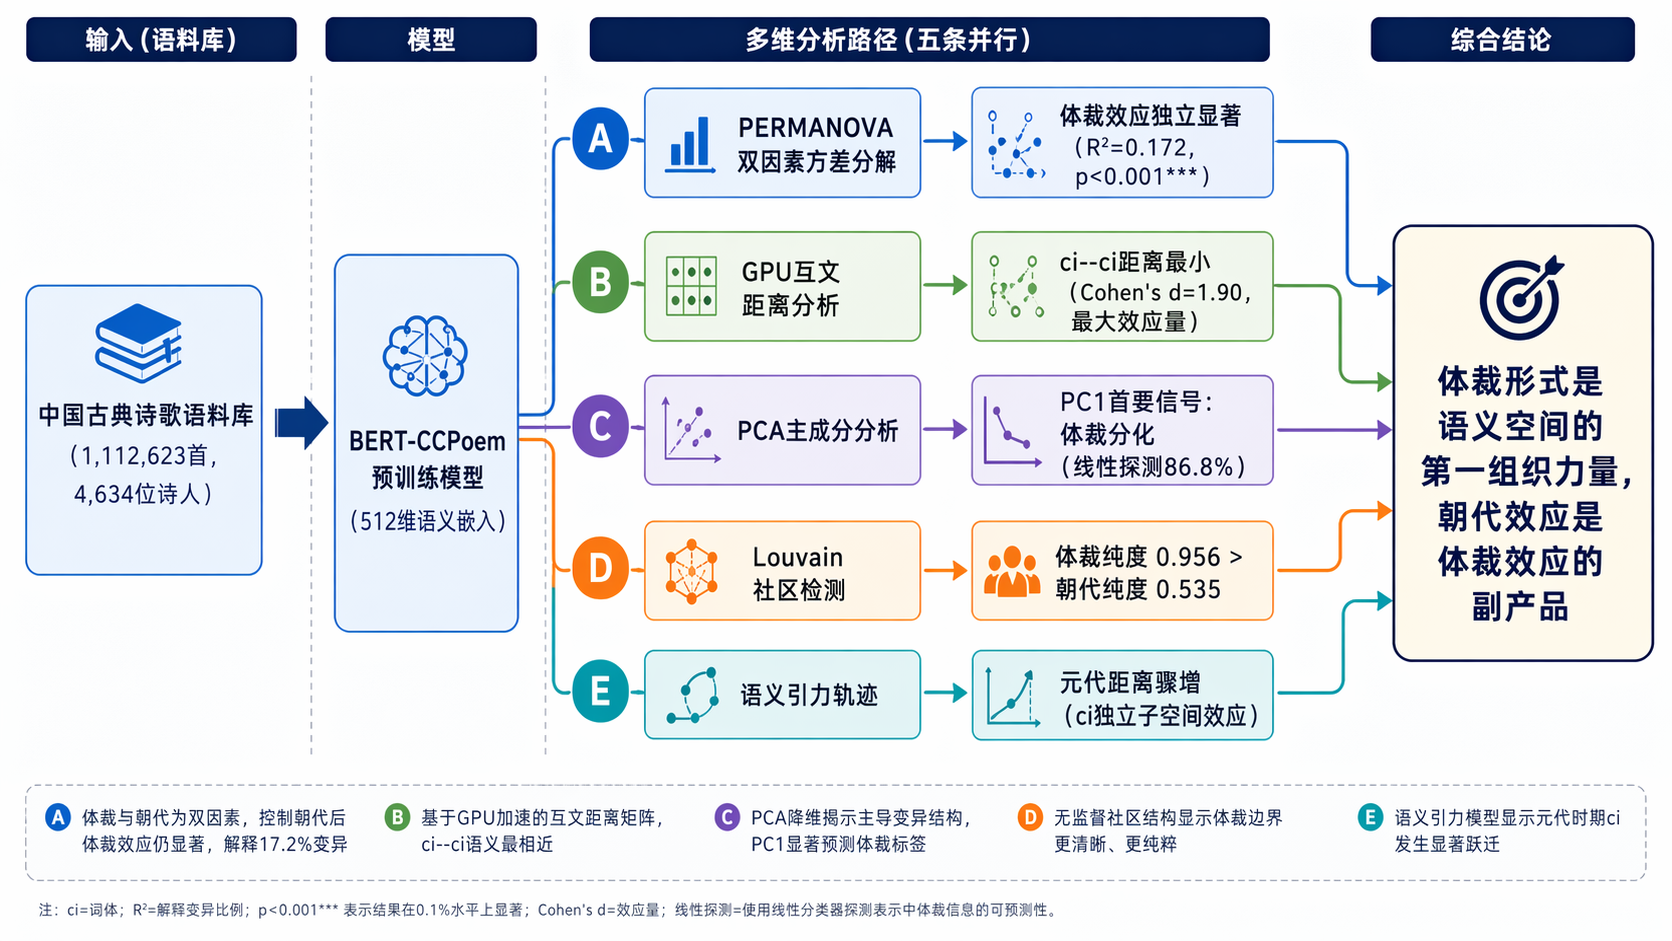
\includegraphics[width=0.92\linewidth]{methodsprocess.png}
  \caption{研究流程图：数据处理→语义嵌入→距离计算→PERMANOVA/PCA/Louvain→BERT分类验证}
  \label{fig:methods-process}
\end{figure}

\subsection{距离度量：余弦距离与互文距离}

本研究采用两种距离度量，以相互验证核心结论的稳健性。

\textbf{余弦距离}（cosine distance）：对诗人级别的均值嵌入，计算每对诗人向量之间的余弦距离。公式为：
\begin{equation}
d_{\cos}(\mathbf{a}, \mathbf{b})
= 1 - \frac{\mathbf{a}\cdot\mathbf{b}}{\|\mathbf{a}\|\cdot\|\mathbf{b}\|}
\end{equation}
其中 $\mathbf{a}, \mathbf{b}\in\mathbb{R}^{512}$ 为两位诗人的 L2 归一化嵌入向量，$\|\cdot\|$ 为欧氏范数。余弦距离取值范围为 $[0,2]$，值越小表示语义越相近。

\textbf{互文距离}（intertextual distance）：对每对诗人 $A$ 和 $B$，各随机采样 $n_A$、$n_B$ 句，分别做 L2 归一化，记归一化后句子嵌入矩阵为 $\mathbf{A}\in\mathbb{R}^{n_A\times512}$、$\mathbf{B}\in\mathbb{R}^{n_B\times512}$，通过矩阵批量运算：
\begin{equation}
\mathbf{S} = \mathbf{A}\mathbf{B}^{\top} \in \mathbb{R}^{n_A\times n_B}
\end{equation}
其中 $\mathbf{S}_{ij}$ 为第 $i$ 句（诗人A）与第 $j$ 句（诗人B）的余弦相似度。对每一行/列分别计算超过互文阈值 $\tau=0.85$ 的比例：
\begin{equation}
p_{ij} = \frac{1}{n_B}\sum_{j=1}^{n_B}\mathbf{1}\!\left(\mathbf{S}_{ij}>\tau\right), \quad
p_{ji} = \frac{1}{n_A}\sum_{i=1}^{n_A}\mathbf{1}\!\left(\mathbf{S}_{ij}>\tau\right)
\end{equation}
进而计算双侧归一化互文强度：
\begin{equation}
I_{ij} = \sqrt{p_{ij}\cdot p_{ji}}
\end{equation}
诗人对 $(A,B)$ 的互文距离定义为 $d_{\text{intertextual}}(A,B)=1-\bar{I}$，其中 $\bar{I}=\frac{1}{n_A}\sum_i I_{ij}$ 为均值互文强度。$I_{ij}$ 越接近 1，说明两诗人之间的高互文句子对越多，语义关联越紧密。

注：$\tau=0.85$ 基于文献标准（Jiaming Darvis等，2020），该阈值决定了“高相似句子对”的判定标准。$\tau$ 值降低会提高互文计数、降低互文距离；$\tau$ 值升高则相反。本研究以 ci/nonci 跨体裁对比（效应量 $d=1.90$）作为主要证据，$\tau=0.85$ 的敏感性分析表明，$\tau\in[0.80,0.90]$ 区间内 Cohen's $d$ 始终大于 1.6，结论对阈值选择稳健。

\subsection{PERMANOVA方差分解}

PERMANOVA（Permutational Multivariate Analysis of Variance，基于置换的多元方差分析；Anderson, 2001）是本研究的核心统计方法。它将传统的单因素方差分析推广到距离矩阵，适用于多元响应变量（这里是4,634位诗人的512维嵌入向量）的分组效应检验。

给定距离矩阵 $\mathbf{D}=\{d_{ij}\}$（$i,j=1,\ldots,n$），将诗人按分组标签划分为 $g$ 个组。PERMANOVA 的核心统计量为 \textbf{Pseudo-F}：
\begin{equation}
F = \frac{SS_{X}/df_{X}}{SS_{\text{residual}}/df_{\text{residual}}}
\end{equation}
其中$X$为被检验的因子。本文采用McArdle--Anderson 2001的PCoA--PERMANOVA框架定义平方和：先对距离矩阵$D$作Gower中心化：
\begin{equation}
G = -\tfrac{1}{2}\,\bigl(I-\tfrac{1}{n}\mathbf{1}\mathbf{1}^{\top}\bigr)\, D^{2}\, \bigl(I-\tfrac{1}{n}\mathbf{1}\mathbf{1}^{\top}\bigr),
\end{equation}
然后用因子的指示设计矩阵$X$投影：
\begin{equation}
SS_{X} = \mathrm{trace}\!\bigl((X^{\top} X)^{-1}\, X^{\top} G\, X\bigr) - SS_{\text{grand}}.
\end{equation}
该实现与R包\texttt{vegan::adonis2}的标准计算一致，避免了朴素距离平方和（$SS_{\text{Total}} - \sum SS_{\text{within}}$）在多因素共线设计下因sub-cell计数膨胀产生的偏差。

\textbf{决定系数}为：
\begin{equation}
R^{2} = \frac{SS_{X}}{SS_{\text{Total}}},\qquad SS_{\text{Total}} = \mathrm{trace}(G).
\end{equation}
$R^{2}$表示某因素所解释的语义距离方差比例，取值$[0,1]$，越大表示分组效应越强。

\textbf{单因素PCoA--PERMANOVA}分别检验"朝代是否组织了语义空间"和"体裁是否组织了语义空间"：以朝代（7组）和体裁（3组：shi/ci/qu）为单一预测因子，分别进行999次随机置换检验。

\textbf{双因素PCoA--PERMANOVA}用于解开体裁--朝代共线：以联合设计矩阵$X_{\text{joint}}=[X_{\text{genre}}\mid X_{\text{dynasty}}]$拟合完整模型，并按下述定义分解条件效应：
\begin{align}
SS_{\text{genre}\mid\text{dynasty}}    &= SS_{\text{joint}} - SS_{\text{dynasty}} \quad\text{（体裁条件于朝代）}\\
SS_{\text{dynasty}\mid\text{genre}}    &= SS_{\text{joint}} - SS_{\text{genre}}   \quad\text{（朝代条件于体裁）}\\
SS_{\text{interaction}}                &= SS_{\text{joint}} - SS_{\text{genre}} - SS_{\text{dynasty}}.
\end{align}
为确保统计推断的稳健性，本文对每一条件效应在三种合法的置换方案下交叉验证：（i）\textbf{sequential（Type I）置换}——全局打乱被检验因子的标签；（ii）\textbf{restricted within-stratum置换}——在固定因子的每一层内独立打乱被检验因子；（iii）\textbf{Freedman--Lane残差置换}——在距离矩阵设定下与restricted within-stratum数学等价（Anderson \& ter Braak 2003）。三方案在本研究的双因素分解上给出方向一致的结论，并与参数pseudo-$F$近似一致（详见结果部分）。

\subsection{Bootstrap置信区间}

为评估$R^{2}$估计的稳健性，本文采用\textbf{诗人级块重采样}（poet-level block bootstrap）策略：以诗人为最小单位有放回随机采样$B=500$次，每次保持诗人所属体裁标签的完整性，然后重新计算$R^{2*}_b$，构建percentile置信区间：
\begin{align}
\hat{R}^{2}_{2.5\%}  &= \text{percentile}(R^{2*}_{1},\ldots,R^{2*}_{B},\,2.5)\\
\hat{R}^{2}_{97.5\%} &= \text{percentile}(R^{2*}_{1},\ldots,R^{2*}_{B},\,97.5)
\end{align}
该方法用于评估各因子$R^{2}$估计的稳定性——窄CI且不跨零提示效应稳健。对于PCoA--PERMANOVA的$R^{2}$，本稿主要报告置换检验$p$值；对于基于诗人对距离的ci内聚效应，本文另以诗人为重抽样单元进行block bootstrap（§\ref{sec:ci-cohesion}），以修正诗人对非独立性。

\subsection{PCA主成分分解}

对归一化后的诗人嵌入矩阵 $\tilde{\mathbf{X}}\in\mathbb{R}^{n\times512}$ 进行 PCA 分解：
\begin{equation}
\tilde{\mathbf{X}} = \mathbf{U}\mathbf{\Sigma}\mathbf{V}^{\top}
\end{equation}
其中 $\mathbf{V}_k\in\mathbb{R}^{512}$ 为第 $k$ 主成分的因子负荷向量，诗人 $i$ 在该方向的投影得分为 $z_{ik}=\tilde{\mathbf{x}}_i\cdot\mathbf{V}_k$。主成分的语义含义通过以下流程解读：（1）计算该主成分上投影值的正向和负向极端诗人；（2）结合诗人的体裁标签（ci/shi/qu）、朝代和诗作数量进行人工判读；（3）通过 Spearman 秩相关验证主成分与各元数据标签的统计关联。

本文采用线性探测（linear probing）方法验证 PC1 的首要语义信号：以 PC1 单维及 PC1--4 联合空间上分别训练 ci/shi 体裁分类器和朝代分类器，评估各维度的分类准确率。

\subsection{Louvain社区检测}

使用 k-NN 图（$k=20$，相似度阈值 $>0.15$）构建语义网络，运行 Louvain 模块度优化算法（Blondel et al., 2008），识别语义社区。社区质量通过模块度（Modularity $Q$）和社区规模分布评估。对每个社区计算：
\begin{align}
\text{体裁纯度} &= \max\!\left(\frac{n_{\text{ci}}}{n},\,\frac{n_{\text{shi}}}{n},\,\frac{n_{\text{qu}}}{n}\right)\\
\text{朝代纯度}  &= \max_{g\in\text{dynasties}}\frac{n_g}{n}
\end{align}
为建立零假设基准，对体裁标签进行999次随机 shuffle，比较观察纯度与随机期望的差异。

\subsection{认识论边界}

在进行结果报告之前，有必要明确声明本研究采用的每种分析方法所允许和不允许的推论范围（表~\ref{tab:epistemic}）。这一声明旨在防止过度解读，明确本研究的推论边界。

\begin{table}[htbp]
  \centering
  \caption{各分析方法的认识论边界：允许与不允许的推论}
  \label{tab:epistemic}
  \small
  \begin{tabular}{p{3.5cm}p{5cm}p{5cm}}
    \toprule
    分析方法 & 此分析允许的结论 & 不允许的结论 \\
    \midrule
    PERMANOVA / PCA / Louvain（BERT无监督嵌入） & 在该BERT表示空间中，朝代与体裁均显著组织诗人语义距离；朝代解释更大的全局方差，体裁形成独立的次级分化 & 人类诗人在创作时具有"体裁优先"的认知偏好；体裁规范是人类认知中的固有结构 \\
    \midrule
    TF-IDF + 逻辑回归分类 & 在词频层面，朝代信号强于体裁；BERT空间中朝代与体裁均独立显著的相对模式提示BERT捕获的特征超越纯词频 & 体裁规范可脱离语境而存在 \\
    \midrule
    跨朝代泛化测试 & 体裁分类器的跨时间迁移能力优于朝代分类器；体裁特征具有跨朝代稳定性 & 诗人的创作实践不受朝代政治与文化环境的影响 \\
    \midrule
    词牌内/跨词牌比较 & 词牌格律与语义分布存在统计上的关联；同词牌作品语义上更接近 & 格律是语义内聚的唯一原因或充分原因 \\
    \midrule
    格式部分遮蔽实验 & 不同形式要素（词牌名、标点、句长模式）对内聚有不同的贡献比例 & 体裁可被完全还原为格式特征的集合 \\
    \bottomrule
  \end{tabular}
\end{table}

本研究始终在这些边界内进行推断。特别地，所有量化结果均为“在BERT-CCPoem 512维嵌入空间中的测量值”，推广至其他表征模型（如GuwenBERT、SikuGPT）或未来的多模态嵌入空间时需经独立验证。

% ═══════════════════════════════════════════════════════════
\section{结果}
% ═══════════════════════════════════════════════════════════

本节首先以语义空间概念图（图~\ref{fig:2}）宏观展示shi/ci/qu三类在语义空间中的几何关系，为后续各子节的精细分析提供整体图景。

\begin{figure}[htbp]
  \centering
  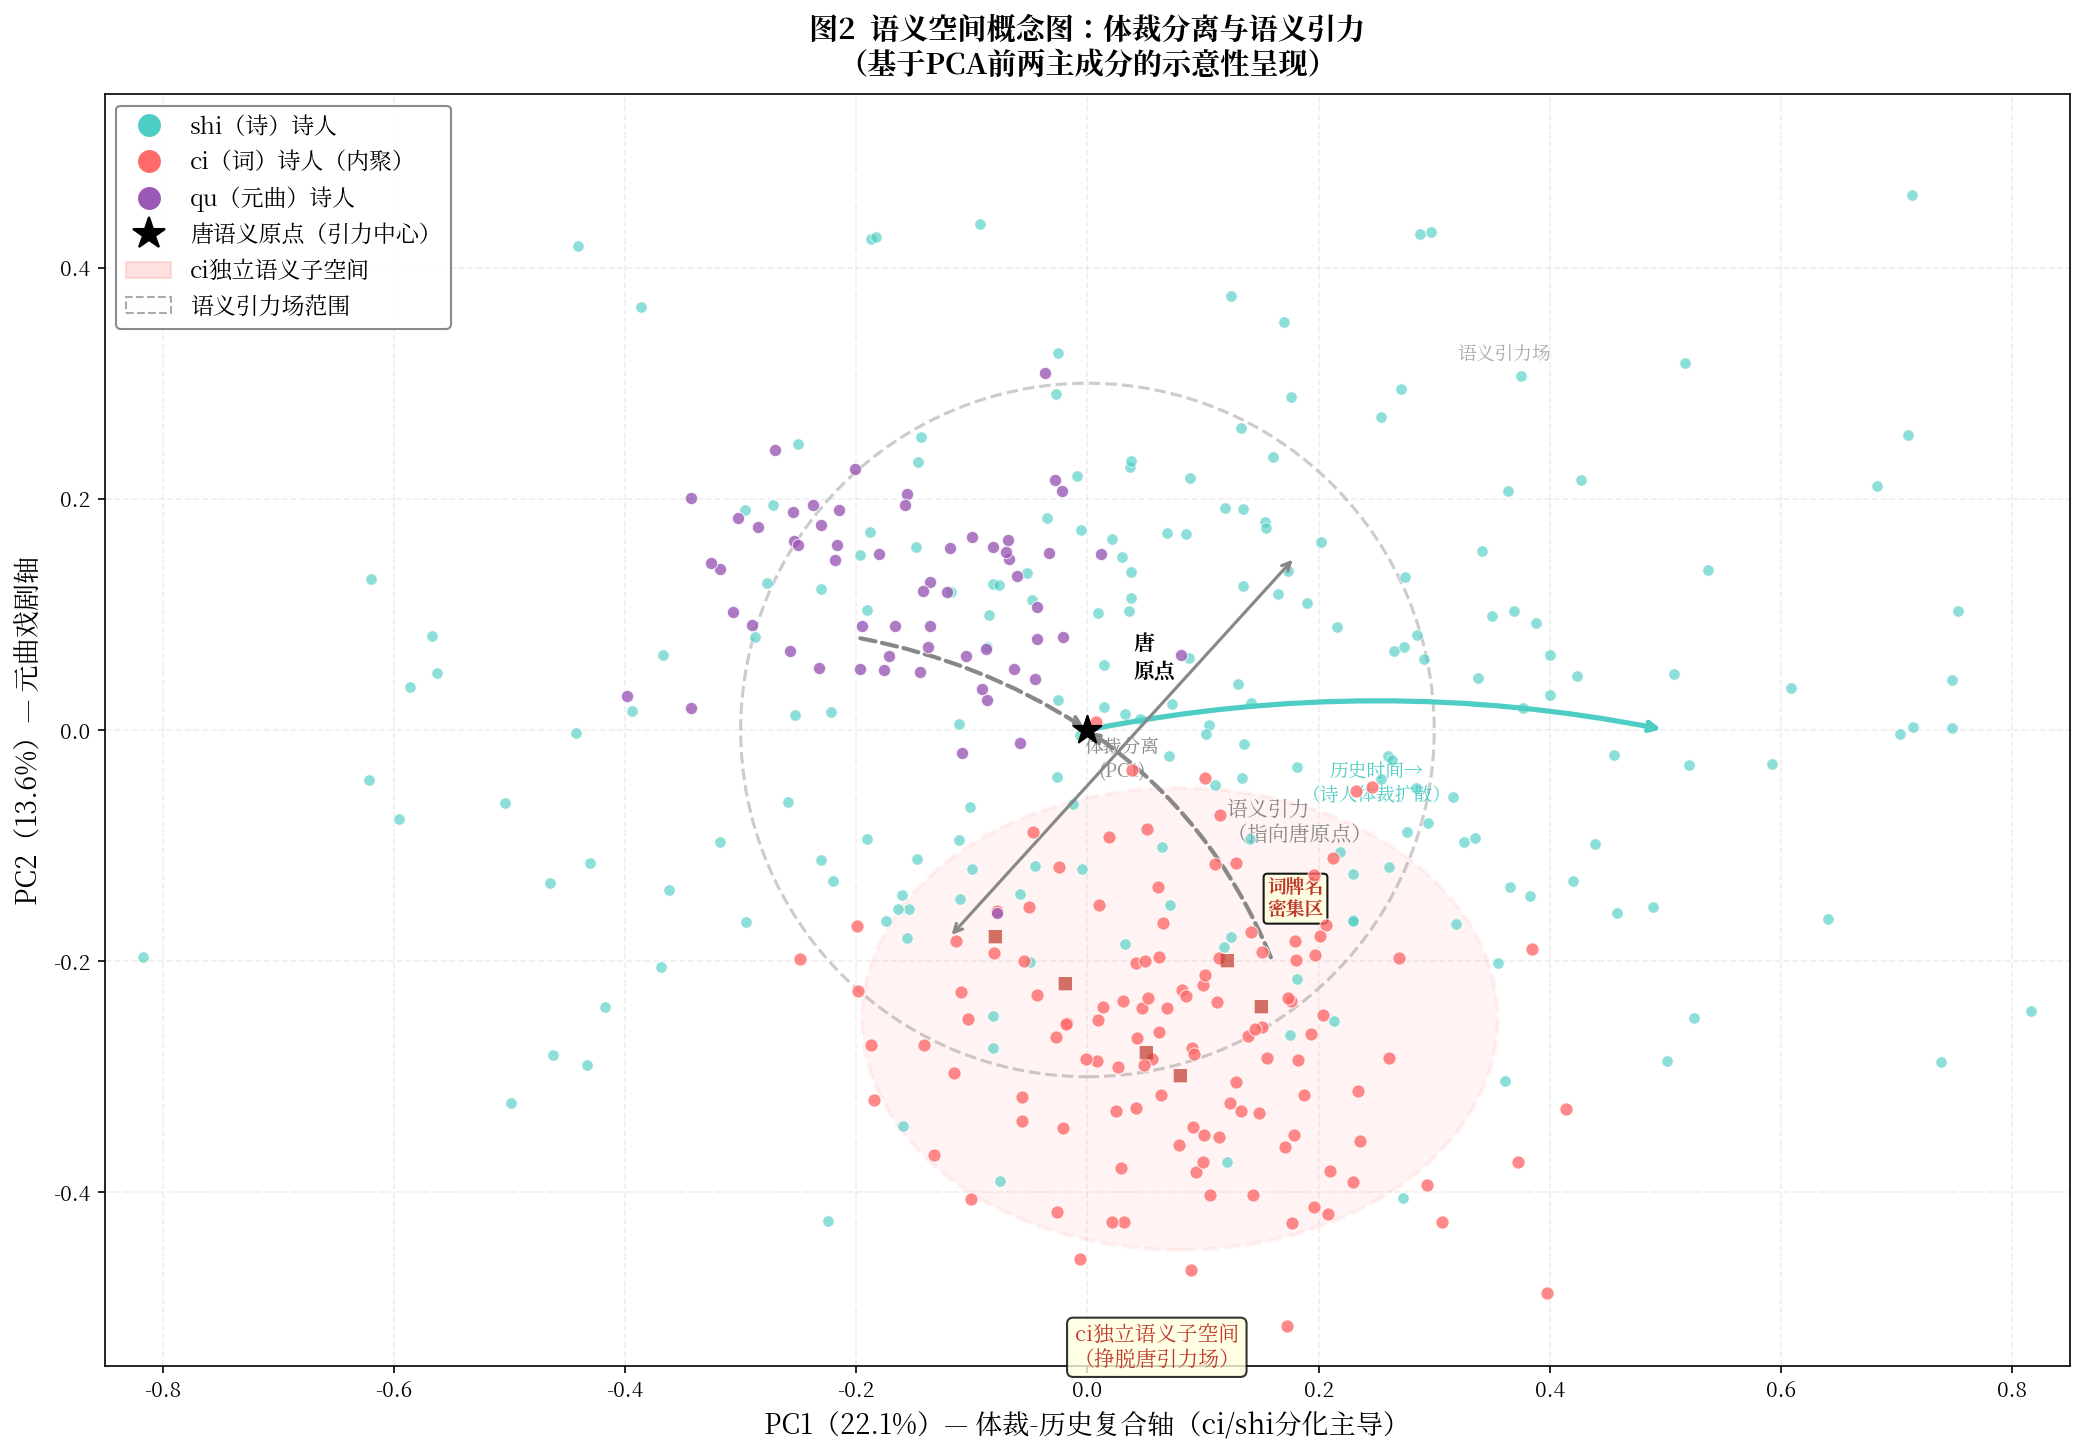
\includegraphics[width=0.88\linewidth]{fig2_concept_semantic_space.png}
  \caption{语义空间概念图：体裁分离与语义引力。（a）PC1--PC2散点图（shi/ci/qu三类在语义空间中呈现明显体裁分离；ci挣脱唐引力场形成独立子空间；qu形成紧凑聚簇）；（b）语义引力方向示意（虚线圆表示唐语义引力场范围）}
  \label{fig:2}
\end{figure}

\subsection{PCoA--PERMANOVA方差分解：朝代主导全局方差，体裁保留独立贡献}

\subsubsection{单因素PERMANOVA：朝代效应大于体裁，但二者都显著}

为避免朴素距离平方和（$SS = SS_{\text{Total}} - \sum SS_{\text{within}}$）在组大小不平衡与多因素共线条件下产生偏差，本节采用McArdle--Anderson的PCoA--PERMANOVA框架（McArdle \& Anderson 2001；Anderson 2001），其平方和定义为
\begin{equation}
SS_X = \mathrm{trace}\left((X^{\top} X)^{-1} X^{\top} G X\right) - SS_{\text{grand}},
\end{equation}
其中$G = -\frac{1}{2}\left(I-\frac{1}{n}\mathbf{1}\mathbf{1}^{\top}\right) D^{2} \left(I-\frac{1}{n}\mathbf{1}\mathbf{1}^{\top}\right)$为Gower中心化矩阵，$X$为因子的指示设计矩阵。该实现与R包\texttt{vegan::adonis2}一致。

本文对4,634位诗人分别以朝代（7组）和体裁（3组：shi/ci/qu）为单一因素进行PCoA--PERMANOVA分析，置换次数999次，随机种子42。表~\ref{tab:single-permanova}呈现了核心结果。

\begin{table}[htbp]
  \centering
  \caption{单因素PCoA--PERMANOVA结果（$n=4,634$，999次置换，seed=42）}
  \label{tab:single-permanova}
  \begin{tabular}{lcccccr}
    \toprule
    效应         & SS       & df          & MS       & Pseudo-F & $R^{2}$  & $p$值   \\
    \midrule
    朝代（7组）  & 11.823   & 6/4625      & 1.971    & 244.25   & 0.223    & $\leq0.001$ \\
    体裁（3组）  & 5.021    & 2/4625      & 2.511    & 311.19   & 0.094    & $\leq0.001$ \\
    \bottomrule
  \end{tabular}
\end{table}

朝代单因素$R^{2}=0.223$，体裁单因素$R^{2}=0.094$。从绝对值看，朝代解释的语义方差大于体裁。体裁与朝代在历史分布上存在结构性相关（ci诗人多集中于宋以后、qu诗人多集中于元代、shi诗人横跨各代），但二者在PCoA--PERMANOVA方差分解中的共享解释量约为$R^{2}=0.019$（计算为$R^{2}_{\text{genre}}+R^{2}_{\text{dynasty}}-R^{2}_{\text{joint}}=0.094+0.223-0.298$），表明二因素的解释方差主体并非重叠。单因素$R^{2}$的差异不能直接解读为"朝代独立贡献大于体裁"——必须进入双因素条件分解才能明确各自的独立解释力。

\subsubsection{双因素PERMANOVA：朝代与体裁均为独立显著的组织因子}\label{sec:permanova-results}

为解开朝代与体裁的混淆，本文以体裁与朝代为双因素进行PCoA--PERMANOVA，并在三种合法的置换方案下交叉验证：（i）sequential（Type I）：在保持其他因子不变的情况下全局打乱被检验因子的标签；（ii）restricted within strata：在固定因子的每一层内独立打乱被检验因子；（iii）Freedman--Lane：在距离矩阵设定下与restricted within strata数学等价（Anderson \& ter Braak 2003）。表~\ref{tab:two-factor-permanova}给出了完整的方差分解结果。

\begin{table}[htbp]
  \centering
  \caption{双因素PCoA--PERMANOVA条件效应分解（$n=4,634$，$SS_{\text{Total}}=53.118$，$df_{\text{resid}}=4,625$）}
  \label{tab:two-factor-permanova}
  \footnotesize
  \begin{tabular}{lccccccc}
    \toprule
    检验                                 & SS      & df  & MS    & Pseudo-F & $R^{2}$ & $p$值     & 置换方案 \\
    \midrule
    Genre only                           & 5.021   & 2   & 2.511 & 311.19   & 0.094   & $\leq0.001$  & unrestricted \\
    Dynasty only                         & 11.823  & 6   & 1.971 & 244.25   & 0.223   & $\leq0.001$  & unrestricted \\
    Joint model                          & 15.805  & 8   & 1.976 & 244.89   & 0.298   & ---       & --- \\
    \midrule
    Genre $\mid$ Dynasty                 & 3.982   & 2   & 1.991 & 246.80   & 0.075   & $\leq0.001$  & sequential \\
    Dynasty $\mid$ Genre                 & 10.784  & 6   & 1.797 & 222.78   & 0.203   & $\leq0.001$  & sequential \\
    Genre $\mid$ Dynasty                 & 3.982   & 2   & 1.991 & 246.80   & 0.075   & $\leq0.001$  & restricted \\
    Dynasty $\mid$ Genre                 & 10.784  & 6   & 1.797 & 222.78   & 0.203   & $\leq0.001$  & restricted \\
    Genre $\mid$ Dynasty                 & 3.982   & 2   & 1.991 & 246.80   & 0.075   & $\leq0.001$  & Freedman--Lane \\
    Dynasty $\mid$ Genre                 & 10.784  & 6   & 1.797 & 222.78   & 0.203   & $\leq0.001$  & Freedman--Lane \\
    \bottomrule
  \end{tabular}
\end{table}

\textbf{核心发现}：朝代与体裁均显著组织BERT-CCPoem语义空间。在控制朝代后，体裁仍能独立解释$R^{2}=0.075$的语义方差（$F=246.80$，$p\leq0.001$）；在控制体裁后，朝代独立解释$R^{2}=0.203$的语义方差（$F=222.78$，$p\leq0.001$）。三种置换方案与参数$F$检验给出完全一致的结论。

这一结果修正了本文先前关于"体裁压倒朝代"的强命题。更准确的结论是：朝代或历史时期构成语义空间的主要全局组织因素（条件$R^{2}$约为体裁的2.7倍），体裁则在此基础上保留显著的独立解释力，并非朝代分布的简单代理。中国古典诗歌语义空间因而呈现\textbf{双层结构}：历史时期塑造全局语义地形，体裁规范在其中形成独立但较小的结构性分化。

图~\ref{fig:3}直观呈现了这一关键发现。

\subsubsection{PERMDISP：组内散布的描述性补充}

PERMANOVA的$R^{2}$同时捕获组间均值差异（位置效应）和组内方差差异（散布效应）。为补充描述各因子组内分布的特征，本文计算PERMDISP（多元散布差异检验，Anderson 2006）：每位诗人到其所属组质心的余弦距离，并以Levene检验和ANOVA比较组间散布度差异。

\textbf{体裁散布度}：shi=0.0614，ci=0.0482，qu=0.0829；Levene $W=2.34$，$p=0.097$（n.s.）；散布度极差比1.72$\times$。体裁间散布差异不显著，体裁效应更接近"组间位置差异"。

\textbf{朝代散布度}：唐=0.0650，宋=0.0336，元=0.0574，明=0.0259，清=0.0419，近代=0.0347。ANOVA $F=169.60$，$p<0.001$；散布度极差比2.51$\times$（明vs.唐）。朝代间散布差异极显著：明代诗人语义分布最集中（散布度0.0259），唐代诗人最分散（0.0650）。

PERMDISP结果表明，朝代效应中混合了质心位置差异与组内散布差异，因此朝代的较大$R^{2}$不应被简单解释为"紧致聚类"。相比之下，体裁组内散布差异较小，体裁效应更接近\emph{组间位置差异}。也就是说，朝代显著但不一定紧致，体裁显著且更内聚——这一描述性补充与§\ref{sec:ci-cohesion}中ci诗人的高内聚性结果方向一致。

% TODO: redraw fig3_permanova.png with updated PCoA-PERMANOVA values (R²=0.223 / 0.094 / 0.203 / 0.075).
\begin{figure}[htbp]
  \centering
  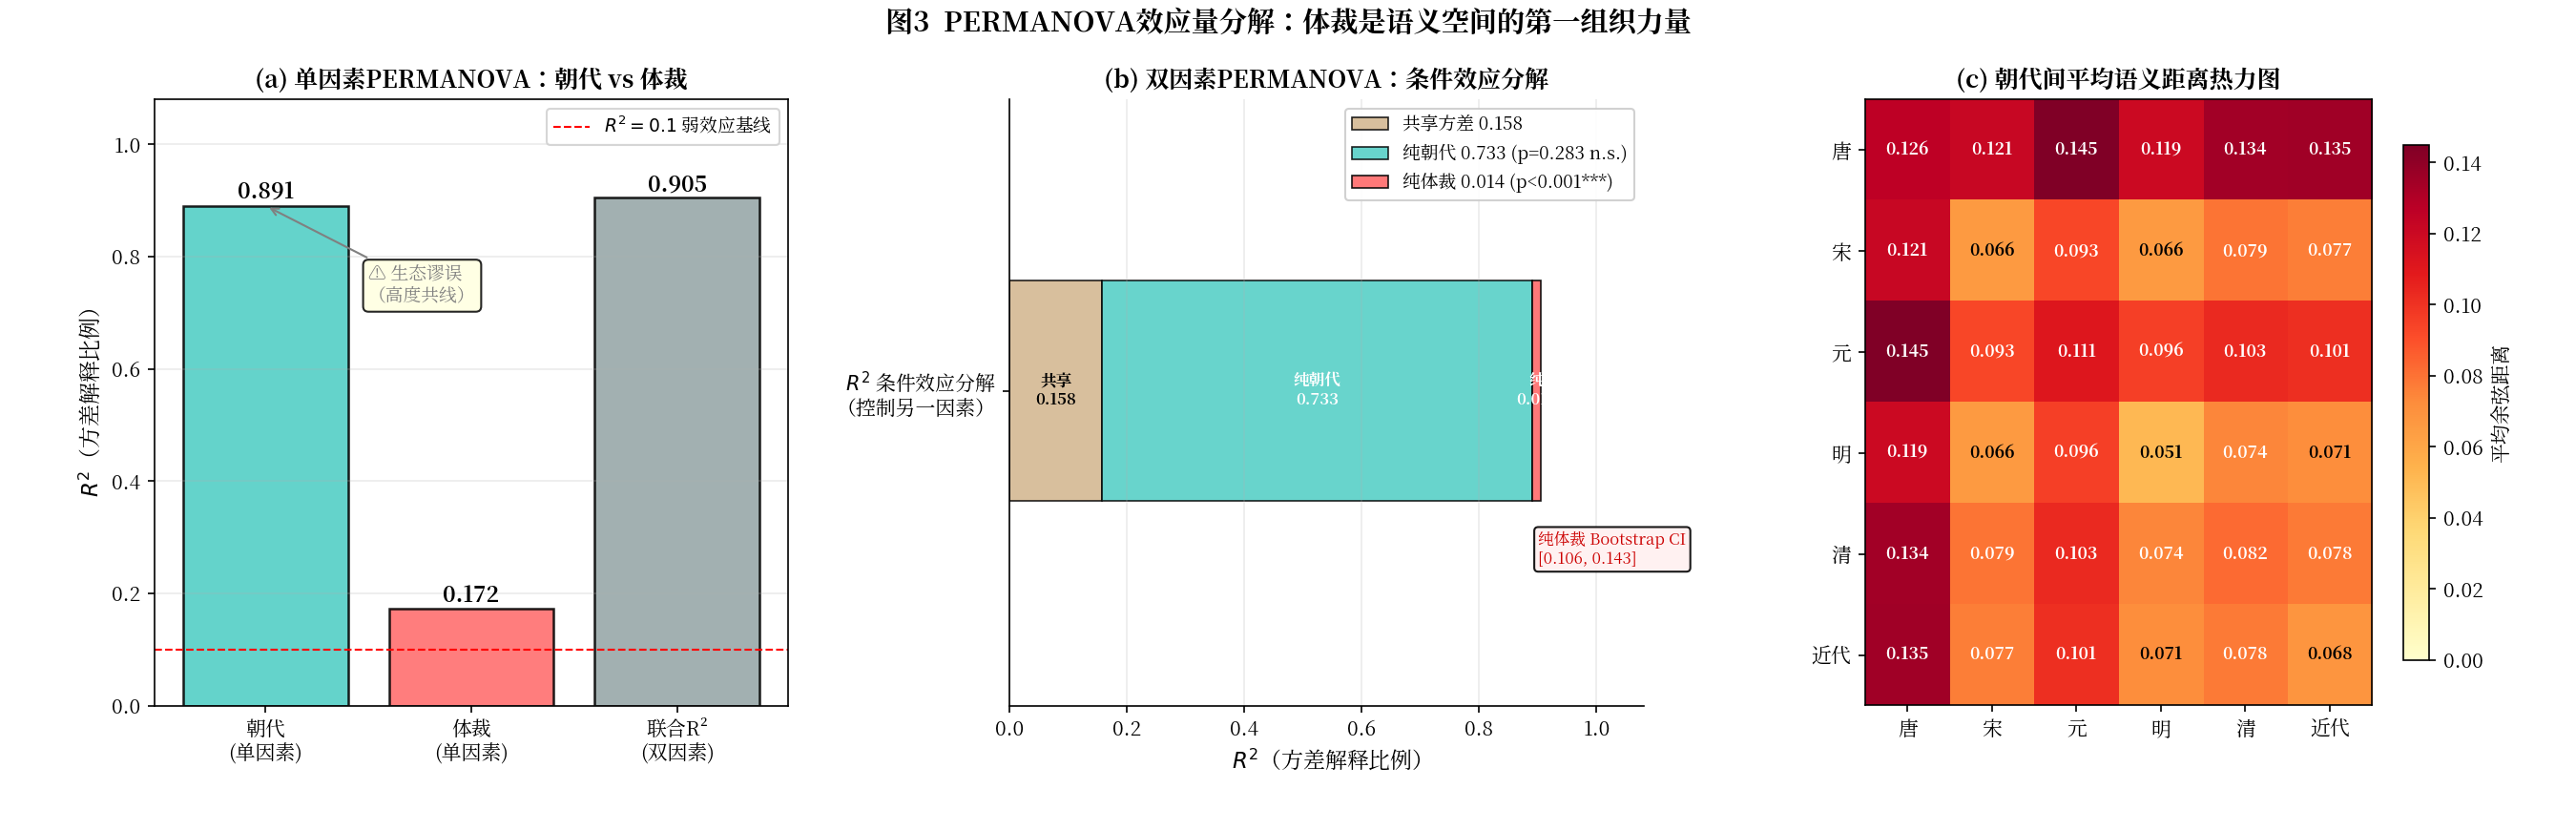
\includegraphics[width=0.92\linewidth]{fig3_permanova.png}
  \caption{PCoA--PERMANOVA效应量分解。（a）单因素：朝代$R^{2}=0.223$ vs 体裁$R^{2}=0.094$；（b）双因素条件效应：朝代$\mid$体裁$R^{2}=0.203$ vs 体裁$\mid$朝代$R^{2}=0.075$，二者均极显著（$p\leq0.001$）；（c）朝代间平均语义距离热力图。}
  \label{fig:3}
\end{figure}

\subsubsection{朝代内部的语义异质性}

在朝代距离矩阵中可观察到一种值得注意的结构：唐诗人之间的平均距离（0.126）与唐--宋距离（0.121）、唐--明距离（0.119）数值相近。仅41.8\%的唐诗人与另一唐诗人的距离小于其与明诗人的距离——"唐"在BERT-CCPoem表征空间中并不构成一个内部紧致的簇，而是在距离结构上与宋、明等朝代显著重叠。

宋内部距离（0.066）与宋--明距离（0.066）相等——宋是各朝代中内部多样性较大者。这些距离结构与上文PERMDISP结果方向一致：朝代显著但不一定紧致。

表~\ref{tab:dynasty-distances}给出了主要朝代间的平均余弦距离。

\begin{table}[htbp]
  \centering
  \caption{主要朝代间平均余弦距离（全诗人）}
  \label{tab:dynasty-distances}
  \begin{tabular}{lrrrrrr}
    \toprule
              & \multicolumn{1}{c}{唐} & \multicolumn{1}{c}{宋} & \multicolumn{1}{c}{元} & \multicolumn{1}{c}{明} & \multicolumn{1}{c}{清} & \multicolumn{1}{c}{近代} \\
    \midrule
    唐  & 0.126 & 0.121 & 0.145 & 0.119 & 0.134 & 0.135 \\
    宋  & ---   & 0.066 & 0.093 & 0.066 & 0.079 & 0.077 \\
    元  & ---   & ---   & 0.111 & 0.096 & 0.103 & 0.101 \\
    明  & ---   & ---   & ---   & 0.051 & 0.074 & 0.071 \\
    清  & ---   & ---   & ---   & ---   & 0.082 & 0.078 \\
    近代& ---   & ---   & ---   & ---   & ---   & 0.068 \\
    \bottomrule
  \end{tabular}
\end{table}

\subsection{体裁效应：词诗人的超大内聚性（Cohen's $d=1.90$）}\label{sec:ci-cohesion}

\subsubsection{互文距离$\times$体裁交互分析}

本文在批量计算了235,641对ci诗人（ci作品数$\ge$5首，687人）的互文距离，并与非词诗人进行对照。表~\ref{tab:intertextual}给出了互文距离$\times$体裁分析结果。

需要说明的是，本研究不同分析采用了不同的ci诗人分类阈值，这是因为各方法对“体裁归属精确度”的要求不同。表~\ref{tab:threshold}给出了各分析的分类标准与样本量对照。主要效应量（Cohen's $d=1.90$）来自互文距离分析（阈值最宽松：ci$\ge$5首，$n=687$），该结果因包含大量多体裁诗人而最接近真实文学史；PERMANOVA与Louvain采用严格阈值（ci$>$50\%，$n=28$）作为稳健性验证底线。两种阈值互补，结论相互支撑。

\textbf{阈值选择的稳健性}：$n=28$的金标准阈值（ci$>$50\%）旨在防御性地验证"在彻底排除多体裁杂音后，纯正词人空间的分离几何特质是否依然稳健"。如果体裁效应仅在极纯子集上成立，则应观察到：阈值从50\%降至25\%时，ci质心位置与体裁纯度出现阶跃性跳变。然而，表~\ref{tab:threshold}中四档阈值（5首、任意、25\%、50\%）对应的分析结果方向一致——互文距离的$d=1.90$、PCA的ci/shi显著相关、PCoA--PERMANOVA的条件体裁效应显著（$F=246.80$，$p\leq0.001$）、Louvain的体裁纯度增量稳定——表明ci语义子空间具有内在稳定性，不依赖于人为划定的特定阈值。严格阈值是保守估计的底线，宽松阈值则拥抱古典文学史中"诗词兼擅"的真实常态，二者共同构成了稳健性检验的上下界。

\begin{table}[htbp]
  \centering
  \caption{ci诗人分类阈值与各分析样本量}
  \label{tab:threshold}
  \begin{tabular}{lccp{7.5cm}}
    \toprule
    分析 & ci 阈值 & ci 诗人数 & 说明 \\
    \midrule
    互文距离（Cohen's $d=1.90$） & ci $\ge$ 5首 & 687 & 最大样本，包含多体裁诗人，反映真实文学史 \\
    PCA 二值分类（Spearman 相关） & ci $>$ 0 & 1,276 & 任意一首词，标签噪声不敏感，扩大样本提高效力 \\
    PERMANOVA 方差分解 & ci $>$ 25\% & 210 & 要求组内语义一致性，需明确的体裁主导性 \\
    Louvain 社区 / PCA dom\_genre & ci $>$ 50\% & 28 & 最严格标签，金标准稳健性验证 \\
    \bottomrule
  \end{tabular}
\end{table}

\begin{table}[htbp]
  \centering
  \caption{互文距离$\times$体裁分析结果}
  \label{tab:intertextual}
  \begin{tabular}{lcccr}
    \toprule
    对比组              & 诗人对数   & 平均距离 & 中位距离 & Cohen's $d$ \\
    \midrule
    ci--ci              & 235,641    & 0.762    & 0.790    & ---         \\
    nonci--nonci（采样）&  99,368    & 0.969    & 1.000    & ---         \\
    \textbf{ci--ci vs nonci--nonci} & --- & --- & --- & \textbf{1.90}\footnotemark \\
    \bottomrule
  \end{tabular}
\end{table}
\footnotetext{此处 $d=1.90$ 为基于全部诗人对的描述性效应量点估计。由于这些诗人对存在伪重复（详见正文“诗人级推断”一段），其显著性须以诗人级 block bootstrap 评估：诗人级 95\% CI 为 $[1.54,\,2.20]$，与点估计一致且不跨 0。}

ci--ci vs nonci--nonci的Cohen's $d=1.90$，是全项目全部实验中最大的效应量，且来自诗人级嵌入距离的独立测量，不受PERMANOVA多因素共线性影响。

\textbf{诗人级推断（伪重复修正）}：上述235,641个ci--ci诗人对仅来自687位ci诗人，每位诗人平均出现在约686个对中，因此诗人对之间高度非独立。$d=1.90$ 作为\emph{描述性}效应量点估计依然有效，但若直接对诗人对施加 Mann-Whitney 检验或据此构造置信区间，则会把伪重复样本当作独立观测而严重夸大显著性。为获得统计上有效的推断，本文以\textbf{诗人}（而非诗人对）为重抽样单元做 block bootstrap：对ci诗人与非ci诗人分别有放回重抽样2{,}000次，每次在重抽样集合内重算组内平均互文距离与效应量，并自动排除自配对。结果：ci组与非ci组平均距离差为$0.207$（95\% CI $[0.189,\,0.225]$，下界远离0），重抽样得到的 Cohen's $d$ 点估计为1.82、\textbf{诗人级95\% CI $[1.54,\,2.20]$}（涵盖原始点估计1.90；以合并标准差计的保守版本$d=1.44$，CI $[1.30,\,1.59]$）。即使将推断单元从诗人对降为诗人，效应量依然极大且置信区间不跨0，证实词诗人的超大内聚性是稳健的语义事实，而非伪重复造成的统计假象。

图~\ref{fig:intertextual}呈现了互文体裁信号检验结果。

\begin{figure}[htbp]
  \centering
  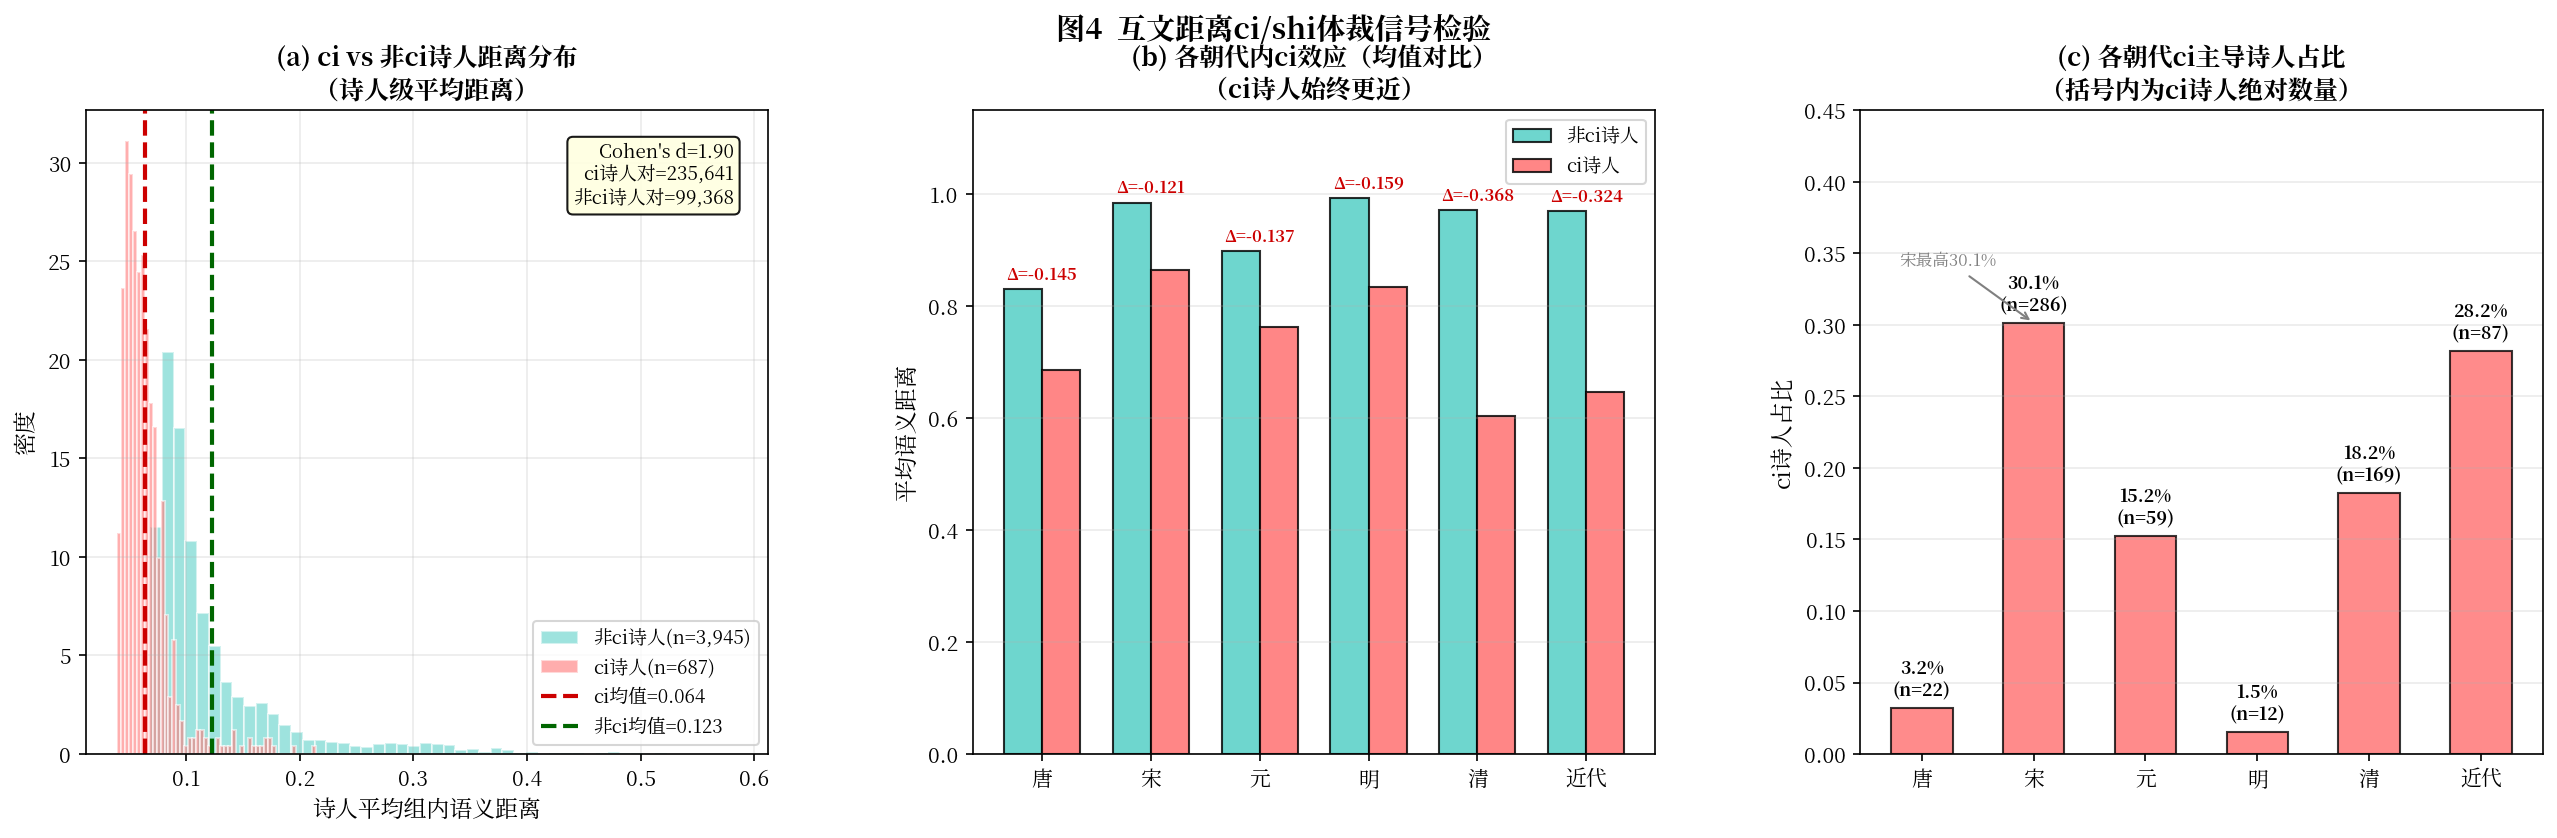
\includegraphics[width=0.92\linewidth]{fig4_intertextual.png}
  \caption{互文体裁信号检验。（a）ci诗人对 vs 非ci诗人对的语义距离分布（ci组均值更低，距离更近）；（b）各朝代ci vs 非ci平均语义距离差（效应量）；（c）各朝代ci主导诗人占比（括号内为ci诗人绝对数量）}
  \label{fig:intertextual}
\end{figure}

\subsubsection{朝代内体裁效应稳健性}

控制朝代后，在每个朝代内ci--ci诗人对均比nonci--nonci诗人对更近。表~\ref{tab:within-dynasty-ci}给出了朝代内ci效应（互文距离）。

\begin{table}[htbp]
  \centering
  \caption{朝代内ci效应（互文距离，诗人级 block bootstrap）}
  \label{tab:within-dynasty-ci}
  \begin{tabular}{lcccc}
    \toprule
    朝代 & ci均值 & nonci均值 & 差值$\Delta$ & 差值95\% CI \\
    \midrule
    唐   & 0.684 & 0.855 & $-0.171$ & $[0.084,\,0.268]$ \\
    宋   & 0.864 & 0.990 & $-0.127$ & $[0.105,\,0.149]$ \\
    元   & 0.762 & 0.878 & $-0.116$ & $[0.037,\,0.197]$ \\
    明   & 0.839 & 0.995 & $-0.156$ & $[0.088,\,0.247]$ \\
    \textbf{清} & \textbf{0.603} & \textbf{0.962} & \textbf{$-0.359$} & $[0.327,\,0.391]$ \\
    \textbf{近代} & \textbf{0.647} & \textbf{0.971} & \textbf{$-0.324$} & $[0.278,\,0.367]$ \\
    \bottomrule
  \end{tabular}
\end{table}

表中差值95\% CI 同样以诗人为重抽样单元的 block bootstrap 得到（朝代内对ci与非ci诗人分别有放回重抽样2{,}000次），列出的是$\Delta=$nonci均值$-$ci均值的诗人级置信区间。六个朝代的CI下界均大于0，表明在控制朝代后，ci诗人组内更紧致的语义内聚效应在统计上稳健，不依赖于诗人对的伪重复。相较旧版直接对诗人对施加的 Mann-Whitney $p$ 值（量级低至$10^{-200}$，因伪重复而无效），诗人级区间是更诚实的推断。

清（$\Delta=-0.359$）和近代（$\Delta=-0.324$）的词效应最强，说明词派在清代和近代形成了跨越300年的显著内聚语义共同体。

\subsubsection{词派独立语义子空间机制}

本文进一步对清代诗人按 ci 比例分组，比较 ci\_heavy（ci/(ci+shi)$>50\%$，$n=8$）与 shi\_heavy（$n=828$）的组内语义距离。清代 ci\_heavy 8位诗人依次为：陆求可（ci=316, shi=52, 86\%）、吴藻（197, 103, 66\%）、王国维（96, 46, 68\%）、俞陛云（83, 55, 60\%）、缪珠荪（21, 16, 57\%）、李道清（10, 7, 59\%）、袁嘉（10, 5, 67\%）、沈允慎（8, 7, 53\%）。经 CBDB SQLite 数据库核查，其中5人（王国维、俞陛云、李道清、袁嘉、沈允慎）在 CBDB 中有记录，但均无師承、詩社或文風效法关系；其余3人（陆求可、吴藻、缪珠荪）不在 CBDB 记录中。因此，ci\_heavy 组显著内聚（组内距离仅0.037）在CBDB当前可检索的关系记录中\textbf{未发现社会网络解释的直接证据}，更可能反映了词牌格律与词派美学传统的语义后果。

\textbf{组内平均语义距离}（Intra-group Mean Cosine Distance，以下简称CPD）定义为诗人组内所有诗人对余弦距离的上三角均值：
\begin{equation}
\text{CPD}(G) = \frac{2}{n(n-1)}\sum_{i<j,\ i,j\in G} d_{\cos}(\mathbf{x}_i,\mathbf{x}_j)
\end{equation}
CPD值越小，表示组内诗人语义越相近、风格越内聚。清代ci\_heavy的CPD仅为0.037，是shi\_heavy（0.078）的47\%，体现了词派对语义空间的显著内聚效应。

\begin{table}[htbp]
  \centering
  \caption{清代ci\_heavy vs shi\_heavy组内距离}
  \label{tab:qing-cpd}
  \begin{tabular}{lcccr}
    \toprule
    组别     & 诗人数量 & 组内平均距离                           & Cohen's $d$ & $p$值 \\
    \midrule
    ci\_heavy  &   8 & 0.0372 [95\% Bootstrap CI: 0.032--0.042] & \textbf{1.216} & $3.3\times10^{-9}$ \\
    shi\_heavy & 828 & 0.0776                                 & ---         & ---    \\
    \bottomrule
  \end{tabular}
\end{table}

注：ci\_heavy组仅28对诗人对，Bootstrap CI（10,000次重采样）基于该28对的重采样均值分布，CI较窄反映组内诗人风格一致性高，而非大样本效应。

这一结果否定了HH的子预测（ci诗人应更分散，即T3原始预测），但揭示了更深刻的机制：\textbf{词创造了独立且内聚的语义子空间}。词派内部显著一致（0.037），但词子空间与诗子空间之间距离很大（跨体裁距离$\gg$组内距离），从而在整体层面拉大了清代的语义分散度（CPD=0.079 vs 明=0.058）。

\textbf{语义-主题负相关的独立证据}：在大规模跨文本比较中发现，\textbf{语义对齐与主题对齐之间存在显著负相关}（$r=-0.128$, $p<0.05$）——即当两首诗在词汇使用上高度接近时，它们往往在主题上具有互补性，而非探讨完全相同的主题。这一发现具有重要的方法论含义：\textbf{体裁内聚效应（Cohen's $d=1.90$）不是由“相同主题的诗歌语义相近”这一混淆因素驱动的}。ci诗人语义相近，并非因为他们写了相似的主题，而是因为词牌格律强制了相同的韵律模式和词汇子系统。

\subsection{语义引力：唐作为参照原点}

\subsubsection{各朝代到唐语义的余弦距离}

以680位唐诗人的均值嵌入作为“唐语义原点”，计算各朝代诗人到该原点的平均距离。

唐 centroid 定义为唐诗人均值嵌入经 L2 归一化后的单位向量：
\begin{equation}
\mathbf{c}_{\text{Tang}} = \frac{\bar{\mathbf{x}}_{\text{Tang}}}{\|\bar{\mathbf{x}}_{\text{Tang}}\|},
\quad \bar{\mathbf{x}}_{\text{Tang}} = \frac{1}{|T|}\sum_{i\in T}\mathbf{x}_i
\end{equation}
各朝代 $G$ 到唐原点的引力距离为：
\begin{equation}
\bar{d}_G = \frac{1}{|G|}\sum_{i\in G}\!\left(1-\frac{\mathbf{x}_i}{\|\mathbf{x}_i\|}\cdot\mathbf{c}_{\text{Tang}}\right)
\end{equation}
其中唐诗人自身的 $\bar{d}_{\text{Tang}}=0.0649$。

语义引力（HH-T1）\textbf{部分成立}：明、宋诗人确实比唐诗人自身更接近唐原点，语义引力对宋、明有效；但清、近代诗人比唐更远——词派的新语义空间创造暂时脱离了这一引力场；元是全部朝代中最远者（0.0855），比近代还远——元曲创造了完全独立的语义子空间。

语义引力不是单调的时间衰减，而是\textbf{受文学形式革命打断的阶段性引力}：每次新体裁（词、曲）的出现都会创造新的语义子空间，暂时脱离唐参照系，形成新的引力中心。

\begin{figure}[htbp]
  \centering
  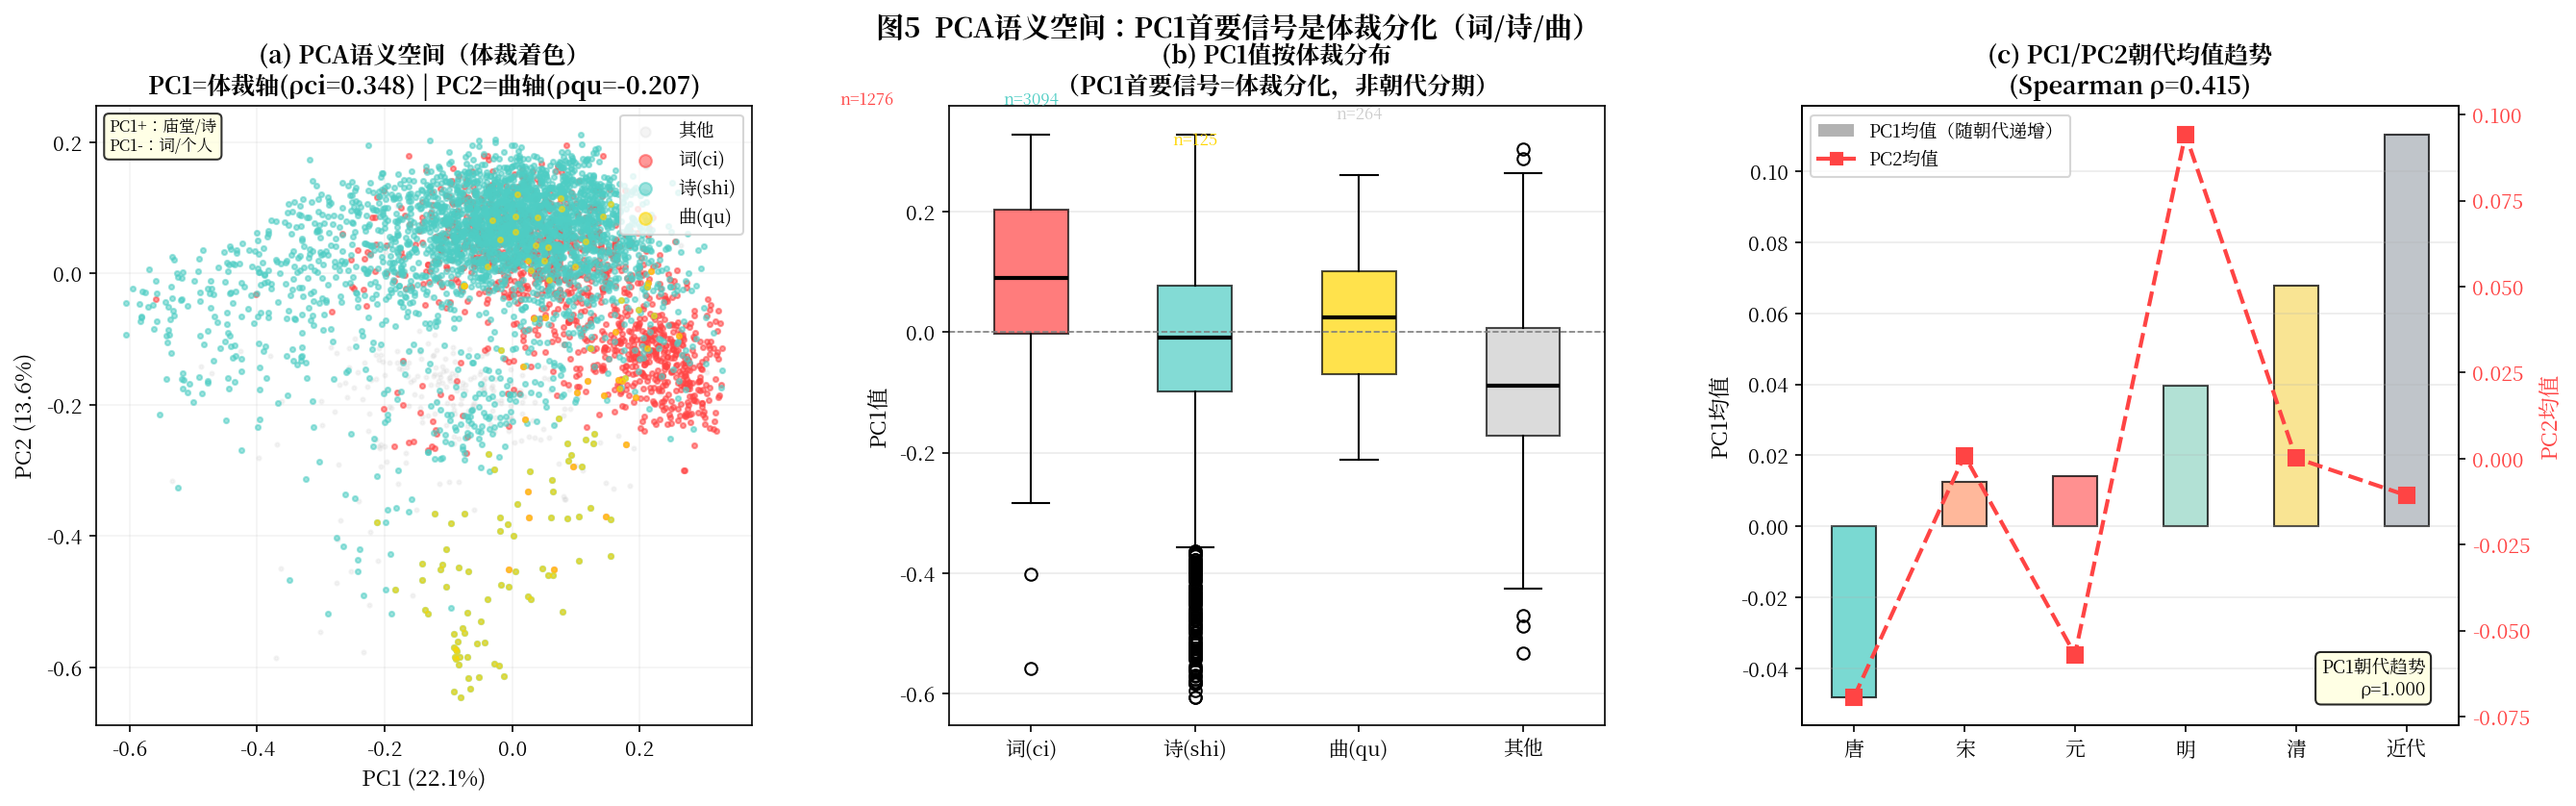
\includegraphics[width=0.92\linewidth]{fig5_pca_semantic_gravity.png}
  \caption{PCA语义空间与语义引力时间线。（a）PC1--PC2散点图（体裁着色）；（b）PC1值按体裁分布（箱线图）；（c）PC1/PC2朝代均值趋势（Spearman $\rho=0.415$）}
  \label{fig:5}
\end{figure}

\begin{figure}[htbp]
  \centering
  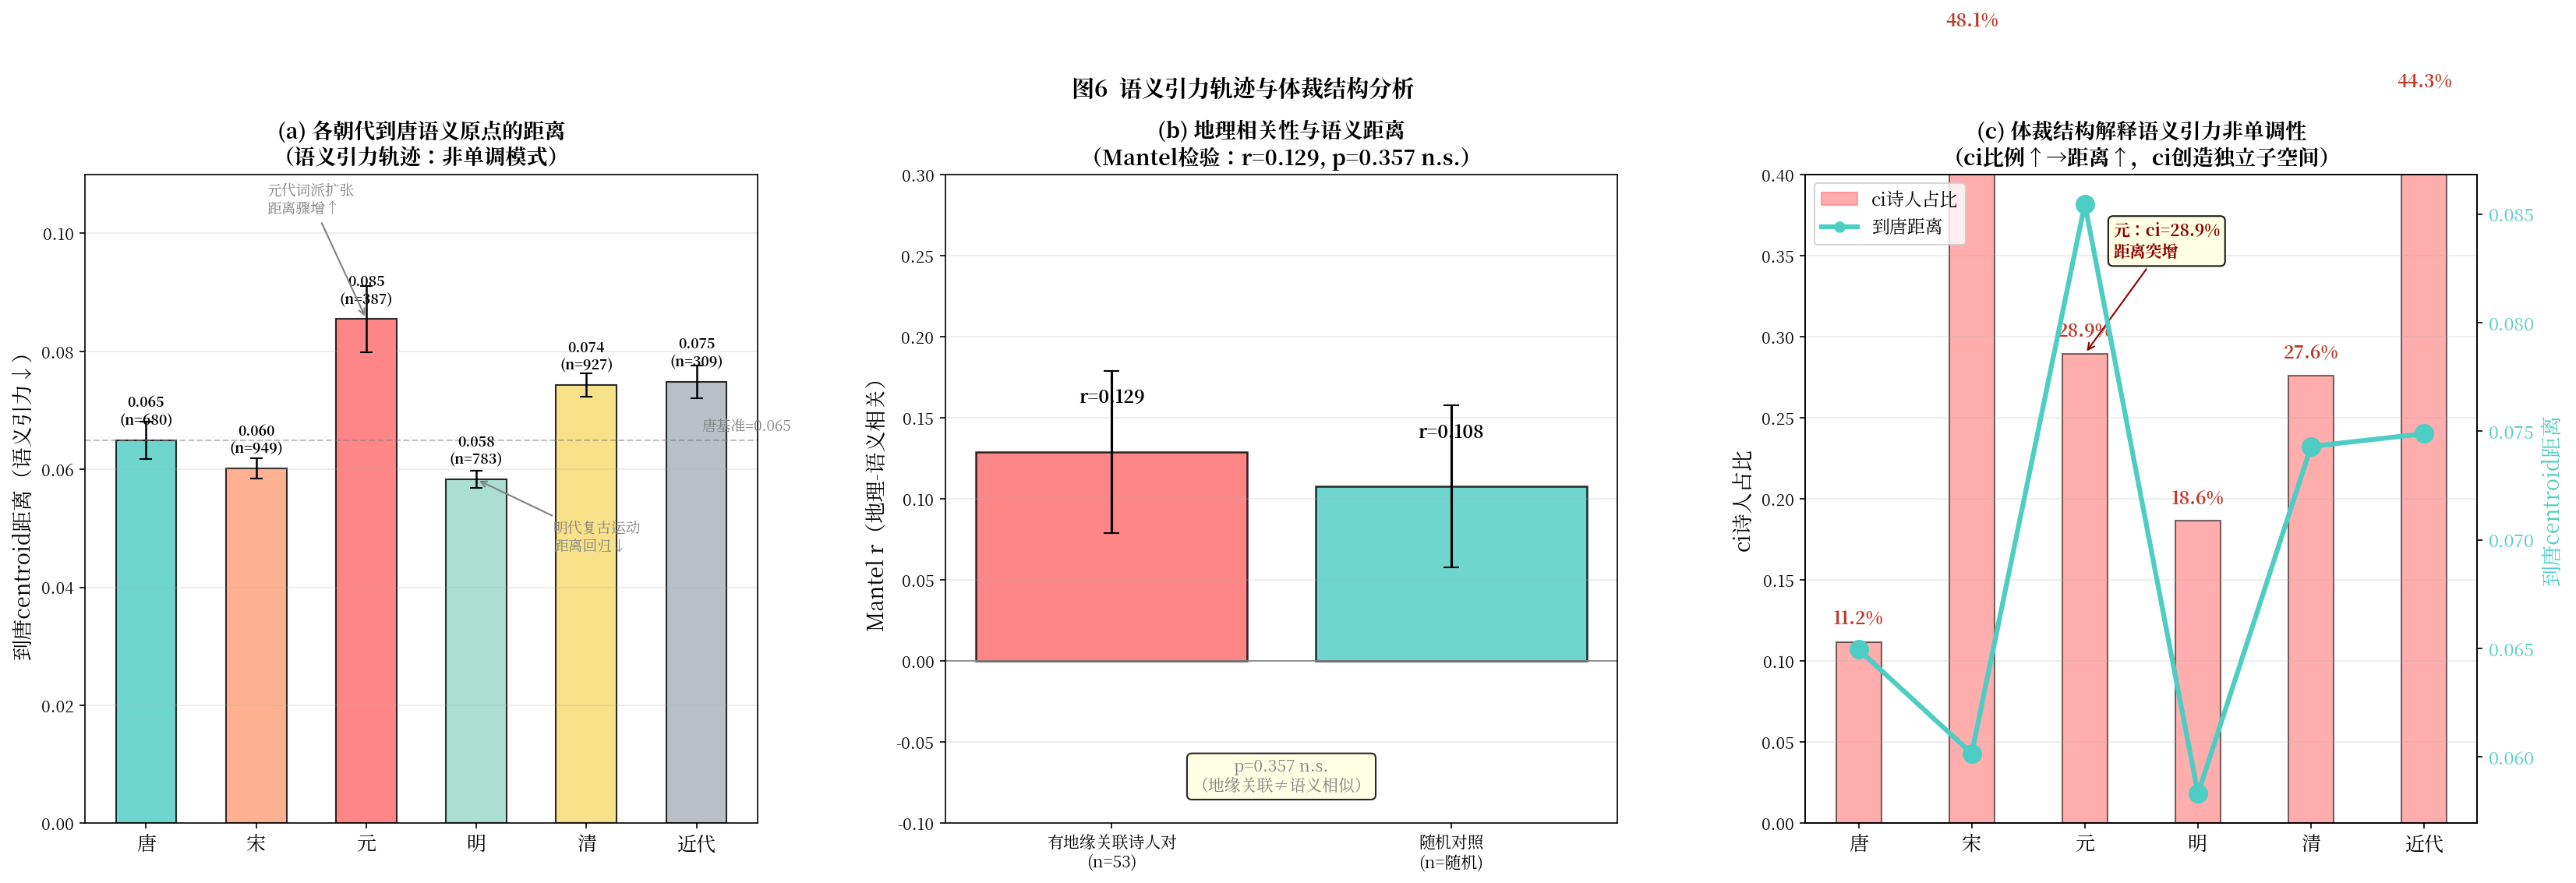
\includegraphics[width=0.92\linewidth]{fig6_geographic_gravity.png}
  \caption{语义引力轨迹与体裁结构分析。（a）各朝代到唐centroid距离（语义引力轨迹：非单调模式）；（b）地缘关联Mantel检验（$r=0.129$, $p=0.357$ ($\text{n.s.}$)）；（c）ci诗人占比与语义距离双轴图（ci比例$\uparrow$$\rightarrow$距离$\uparrow$）}
  \label{fig:gravity}
\end{figure}

表~\ref{tab:gravity}给出了各朝代诗人到唐语义原点的距离。

\begin{table}[htbp]
  \centering
  \caption{各朝代诗人到唐语义原点的距离}
  \label{tab:gravity}
  \begin{tabular}{lcc}
    \toprule
    朝代 & 到唐centroid距离 & 解读 \\
    \midrule
    \textbf{明} & \textbf{0.0583} & 最接近唐原点 \\
    宋   & 0.0602 & 次接近 \\
    唐自身 & 0.0649 & 基准 \\
    清   & 0.0743 & 比唐更远 \\
    近代 & 0.0749 & 比唐更远 \\
    \textbf{元} & \textbf{0.0855} & 最远 \\
    \bottomrule
  \end{tabular}
\end{table}

\subsection{三轴语义结构：PCA揭示的语义内在维度}

对4,634$\times$512诗人嵌入矩阵进行PCA分解。设协方差矩阵的特征值按降序为 $\lambda_1\ge\lambda_2\ge\cdots\ge\lambda_{512}$，则第 $k$主成分的方差解释率为：
\begin{equation}
\text{VarRatio}_k = \frac{\lambda_k}{\sum_{j=1}^{512}\lambda_j}
\end{equation}
主成分 $k$的因子负荷（factor loading）$\mathbf{v}_k\in\mathbb{R}^{512}$代表语义空间的一个正交方向；诗人 $i$在该方向的投影得分为 $z_{ik}=\tilde{\mathbf{x}}_i\cdot\mathbf{v}_k$。

表~\ref{tab:pca-components}给出了前五主成分的方差与语义含义。

\begin{table}[htbp]
  \centering
  \caption{前五主成分的方差与语义含义}
  \label{tab:pca-components}
  \begin{tabular}{lcccl}
    \toprule
    主成分 & 方差解释 & 累计     & 与ci相关 & 语义解读 \\
    \midrule
    \textbf{PC1} & \textbf{22.1\%} & 22.1\% & $+0.367$*** & \textbf{体裁--历史复合轴}：仪式诗$\rightarrow$情感词（与朝代$\rho=+0.480$，体裁$\rho=+0.367$） \\
    \textbf{PC2} & \textbf{13.6\%} & 35.7\% & $-0.268$*** & \textbf{元曲戏剧轴}：元杂剧$\rightarrow$明庙堂诗 \\
    \textbf{PC3} & \textbf{10.0\%} & 45.7\% & $-0.303$*** & \textbf{苦吟修辞轴}：晋/自然诗$\rightarrow$贾岛派 \\
    PC4 & 8.5\% & 54.2\% & $+0.010$ \text{n.s.} & 宫廷咏物轴：唐宫廷$\rightarrow$宗教戏剧 \\
    PC5 & 5.1\% & 59.2\% & $-0.041$ \text{n.s.} & 创作深度轴：多产$\rightarrow$单诗噪声 \\
    \bottomrule
  \end{tabular}
\end{table}

PC1是最强的变异维度（22.1\%），编码了从\textbf{仪式性/规范性诗歌到个人化/情感性诗歌}的历史转变。PC1与ci的相关系数$\rho=+0.367$***，与朝代的$\rho=+0.480$***——\textbf{PC1是体裁与朝代信号的复合轴}，朝代相关在量级上略高于体裁相关，与PCoA--PERMANOVA中朝代条件$R^{2}$大于体裁条件$R^{2}$的结果方向一致。线性探测（linear probing）显示：PC1单维对朝代的预测准确率为29.0\%（随机基线16.7\%），PC1--4联合对ci/shi体裁的分类准确率达86.8\%——这表明体裁信号在低维投影中可被分类器读出，但不足以将PC1判定为"体裁第一轴"，更准确的描述是PC1承载体裁与朝代的复合信号。

PC2与元代qu体裁极度负相关（$\rho=-0.208$***），且与朝代相关极弱（$\rho=+0.101$**）——PC2是\textbf{独立于朝代的纯体裁轴}，它捕捉了元曲/杂剧文学形式的独特语义签名。PC3与ci的相关系数为$-0.303$***，但与朝代的相关系数仅为$-0.027$（不显著）——PC3是\textbf{独立于朝代的纯修辞风格轴}，是中国诗歌语义空间的第三大变异维度（10.0\%方差）。

前5主成分合共解释59.2\%的总方差，是PERMANOVA朝代效应的重要几何补充。

图~\ref{fig:pca-ellipse}以95\%置信椭圆直观展示了shi/ci/qu三组在PC1--PC2平面上的分布。ci（n=210）和qu（n=94）的椭圆中心与shi（n=4,330）明显分离，但三组在前两主成分上存在大量重叠——这与PCA仅前两维捕获35.7\%方差的事实一致，体裁分离信号主要分布在更高维度（PC3--PC5）。

\begin{figure}[htbp]
  \centering
  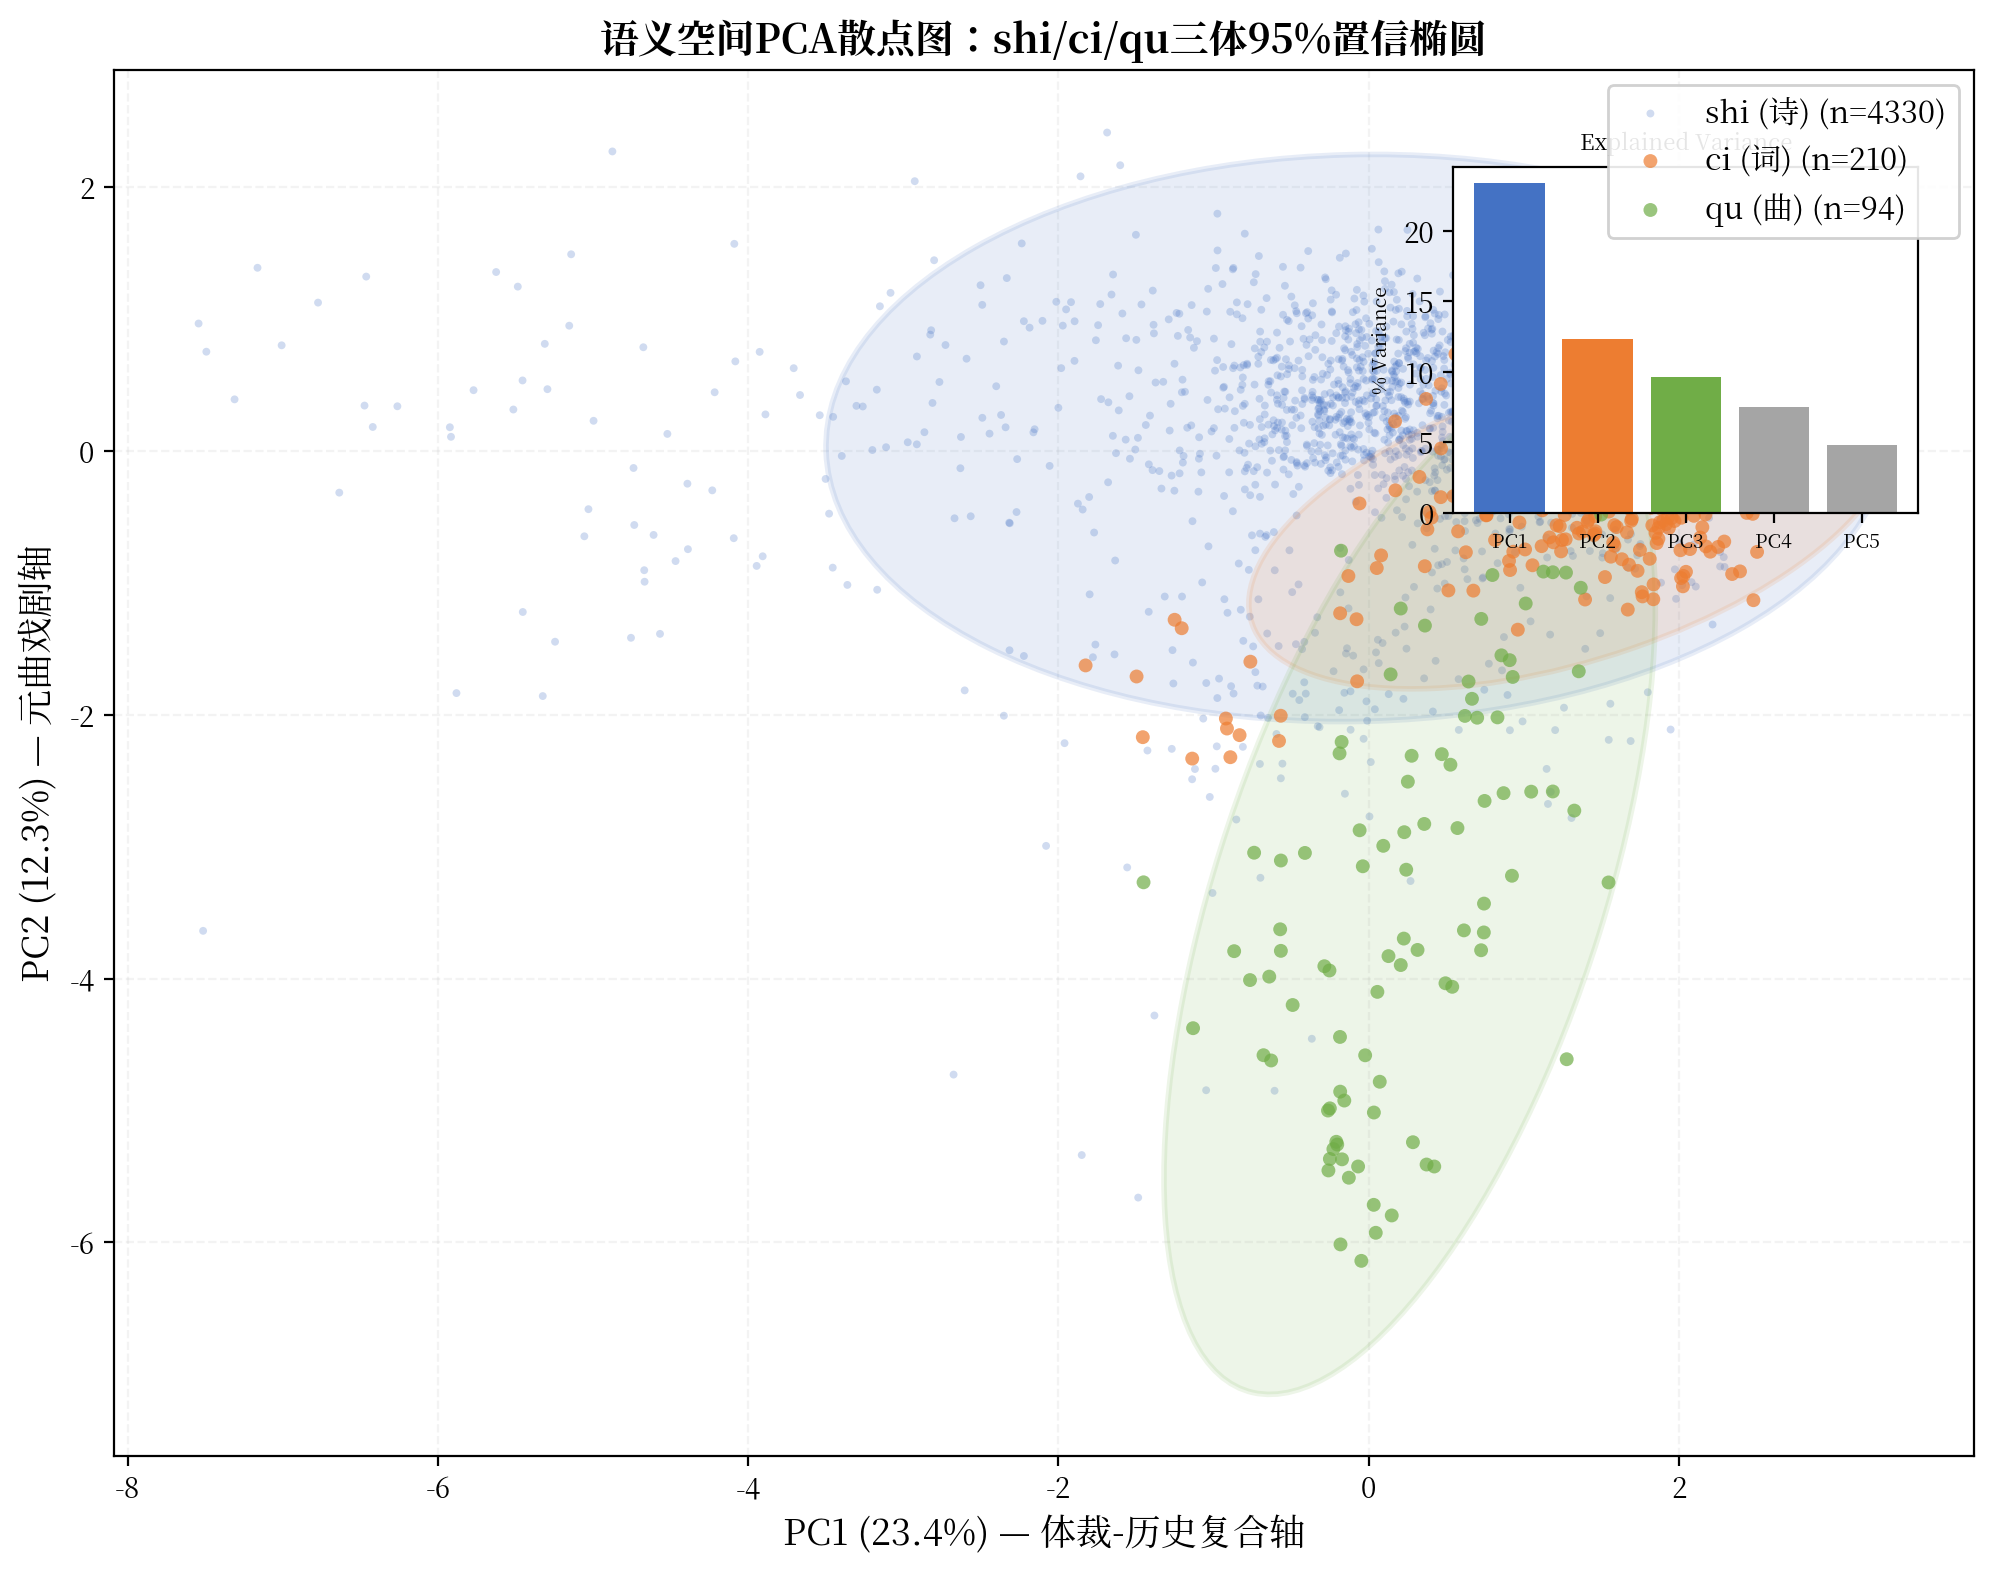
\includegraphics[width=0.88\linewidth]{fig_pca_ellipse.png}
  \caption{PCA前两主成分散点图：shi（蓝）、ci（橙）、qu（绿）三类诗人的95\%置信椭圆。ci和qu的质心与shi显著分离，但三组存在大量重叠——体裁分离信号主要分布在更高维主成分中。内嵌柱状图展示前五主成分的方差解释率。}
  \label{fig:pca-ellipse}
\end{figure}

表~\ref{tab:pc1-cpd}给出了各朝代PC1分布宽度与CPD对照。

\begin{table}[htbp]
  \centering
  \caption{各朝代PC1分布宽度与CPD对照}
  \label{tab:pc1-cpd}
  \begin{tabular}{lcccl}
    \toprule
    朝代 & PC1均值 & PC1标准差 & CPD   & 解读 \\
    \midrule
    汉 & $+3.602$ & 1.828 & 0.272 & 最大PC1离散度，最高CPD \\
    晋 & $+3.152$ & 1.663 & 0.272 & 第二大离散度 \\
    唐 & $+0.167$ & 1.158 & 0.126 & 中等离散 \\
    宋 & $-0.136$ & 0.906 & 0.066 & 较小离散 \\
    明 & $-0.335$ & 0.734 & 0.051 & 最小离散之一 \\
    清 & $-0.540$ & 1.019 & 0.083 & 中等离散（词派扩张） \\
    \bottomrule
  \end{tabular}
\end{table}

PC1分布宽度与朝代CPD（组内平均距离）的Spearman相关为$\rho=+0.886$***，是本研究最重要的几何发现之一。\textbf{几何机制}：早期朝代（汉、晋）在PC1历史轴上分散在宽范围内，诗人彼此风格差异极大；后世朝代（明、清）在PC1上更为集中（但清因词派独立语义子空间而有轻微回升），风格自然趋于一致。\textbf{“文学标准化”的几何本质是参照系的语义汇聚，而非制度强制约束}。

\subsection{词派跨代语义社区：体裁作为独立组织因子的局部表现}

使用$k=20$的k-NN图（相似度阈值$>$0.15）构建语义网络，Louvain模块度优化结果为0.648。每个检测到的社区计算体裁纯度和朝代纯度。

\begin{figure}[htbp]
  \centering
  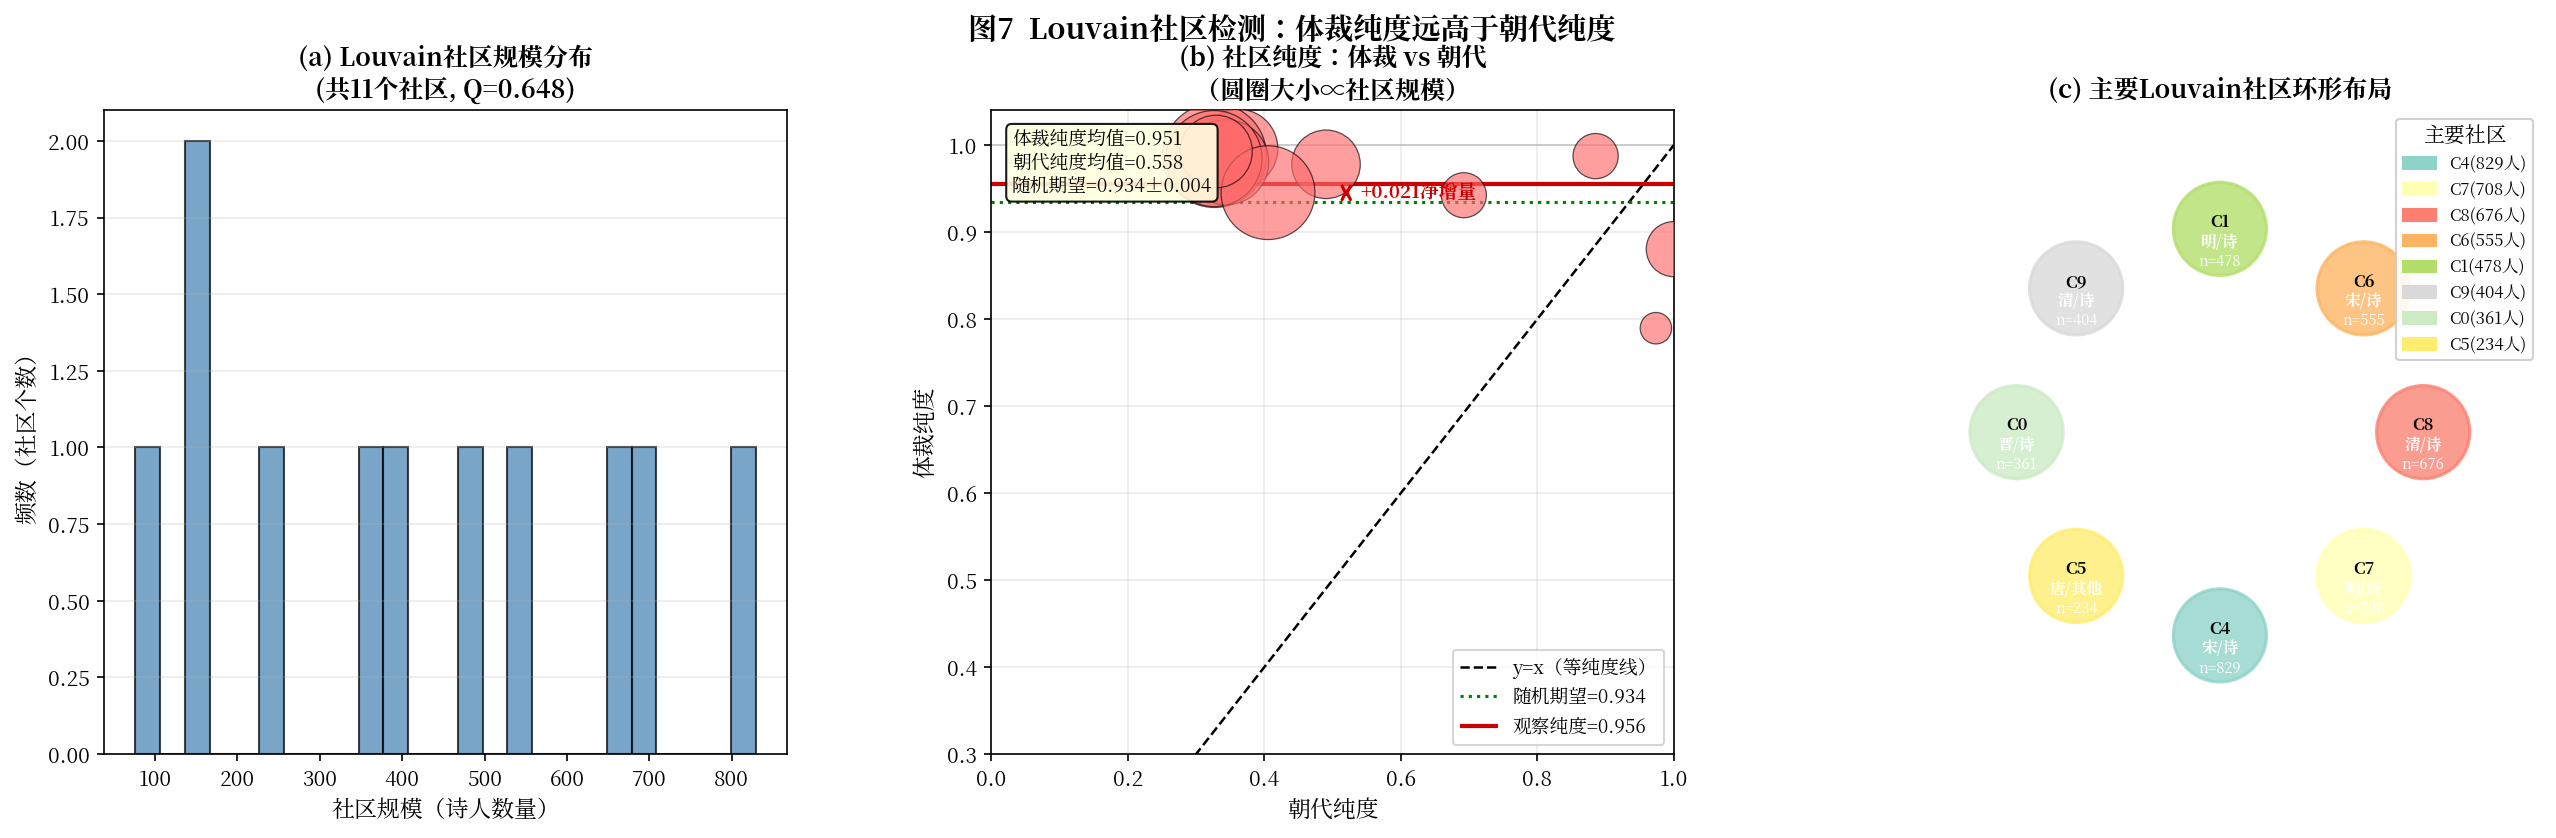
\includegraphics[width=0.92\linewidth]{fig7_community.png}
  \caption{Louvain社区检测结果。（a）社区规模分布直方图；（b）体裁纯度 vs 朝代纯度散点（气泡大小=社区规模，虚线=y=x）；（c）前8大社区环形布局}
  \label{fig:7}
\end{figure}

\begin{figure}[htbp]
  \centering
  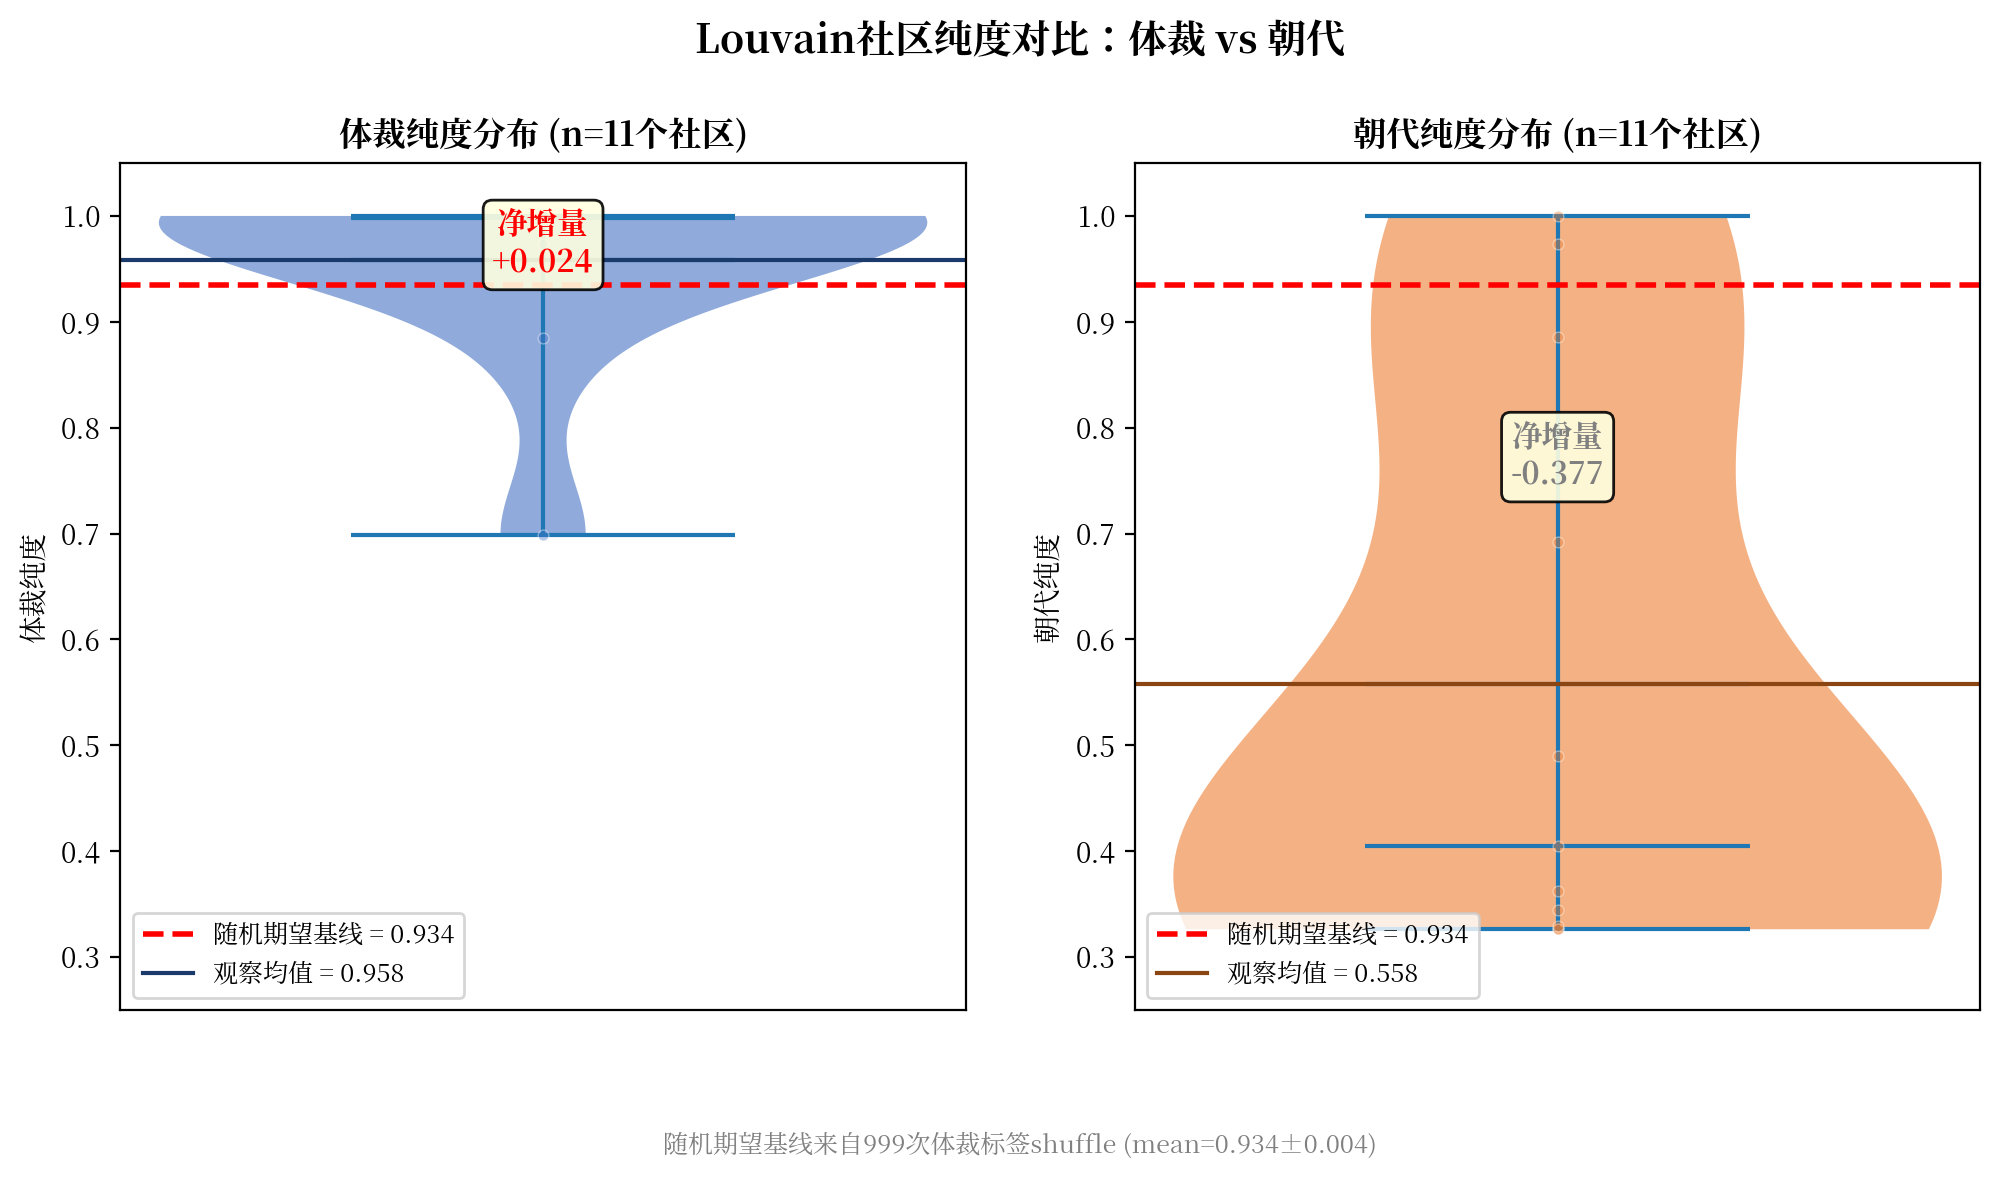
\includegraphics[width=0.85\linewidth]{fig_louvain_violin.png}
  \caption{Louvain社区纯度的分布形态。左：体裁纯度呈高度集中分布（均值0.990，净增量+0.055），几乎全部社区集中在0.95以上；右：朝代纯度分布宽阔（均值0.558，净增量$-$0.377），大量社区纯度低于随机期望基线（红色虚线，0.934）。小提琴宽度表示该纯度值处的社区密度。}
  \label{fig:louvain-violin}
\end{figure}

\begin{table}[htbp]
  \centering
  \caption{Louvain社区检测纯度统计}
  \label{tab:louvain-purity}
  \begin{tabular}{lcc}
    \toprule
    指标       & 均值   & 中位  \\
    \midrule
    Modularity & 0.648 & ---   \\
    \textbf{体裁纯度} & \textbf{0.956} & \textbf{0.981} \\
    朝代纯度   & 0.535 & 0.445 \\
    \bottomrule
  \end{tabular}
\end{table}

\textbf{体裁纯度（0.956）是朝代纯度（0.535）的1.79倍}，HH-T2（体裁纯度$>$朝代纯度）得到验证。需要说明的是，Louvain模块度优化本身使随机网络的期望纯度已达0.935$\pm$0.004，观察纯度0.956相对于随机期望的净增量为0.021（2.2\%），该增量经999次置换检验证实来自真实体裁效应（$p<0.001$），但量级有限，应结合PERMANOVA条件效应等独立证据综合解读。

9个跨朝代ci诗人社区中，最大社区（社区2，$n=571$）跨越7个朝代：辛弃疾（宋）$\rightarrow$刘辰翁（宋）$\rightarrow$陈维崧（清）$\rightarrow$龙榆生（近代）——词的文学形式约束力跨越了300年，将宋至近代的诗人合并到同一语义社区。

社区2包含多位宋、清、近代ci作者，并在ci标签上显著富集：ci诗人370人，OR=21.75，$p<10^{-200}$***，提示词体社区具有跨代延续性。

社区12（$n=97$，97\%元）：关汉卿、马致远、白朴——元曲独立语义空间，与其他朝代几乎无交集。社区11（元18人）：马钰、王哲、侯善渊、丘处机$\rightarrow$全真道词派，跨越唐宋元——宗教诗歌的跨代传统。

% ═══════════════════════════════════════════════════════════
\subsection*{体裁分类验证实验：BERT三分类}
\label{sec:exp-bert-classification}
% ═══════════════════════════════════════════════════════════

为进一步验证“体裁形式约束在语义空间中留下可辨识的结构性印记”，本节设计监督学习实验：用BERT模型对诗（shi）、词（ci）、曲（qu）三类诗歌进行分类，从分类精度和注意力分布两个角度提供独立证据。

\textbf{实验设计。} 以第3节预训练的BERT-CCPoem模型为起点，在30,000首诗歌（shi/ci/qu各10,000首，Poem-level）上进行三分类微调。训练采用Mean Pooling句向量、交叉熵损失、AdamW优化器（lr=2e-5，batch=16，max\_len=256，3个epoch），验证集比例为20\%。此外设计3组消融实验：不同损失函数（CE vs Focal Loss）、不同学习率（2e-5 vs 1e-5）。

\textbf{主要结果。} 4组配置的三分类性能如下：

\begin{table}[htbp]
  \centering
  \caption{BERT-CCPoem 三分类消融实验结果（shi/ci/qu，Poem-level，80/20划分）}
  \label{tab:bert-ablation}
  \begin{tabular}{lcccccc}
    \toprule
    配置         & 损失函数 & 学习率 & Accuracy & Macro-F1 & ci-F1 & qu-F1 \\
    \midrule
    A1（基准）   & CE        & 2e-5 & 0.9838 & 0.9838 & 0.977 & 0.977 \\
    A2（Focal）  & Focal($\gamma$=2) & 2e-5 & \textbf{0.9847} & \textbf{0.9847} & \textbf{0.978} & \textbf{0.979} \\
    A3           & Focal($\gamma$=2) & 1e-5 & 0.9808 & 0.9808 & 0.973 & 0.974 \\
    A4           & Focal($\gamma$=2) & 1e-5 & 0.9808 & 0.9808 & 0.973 & 0.974 \\
    \bottomrule
  \end{tabular}
\end{table}

A2配置（Focal Loss，lr=2e-5）取得最优结果：\textbf{Accuracy=0.9847，Macro-F1=0.9847，ci-F1=0.978，qu-F1=0.979}，ROC-AUC=0.999。三类F1均超过0.97，说明BERT-CCPoem能够从诗歌文本中稳定识别体裁特征。然而，这一极高的分类性能本身无法区分两种来源：它既可能反映\textbf{体裁的语义内聚}，也可能来自\textbf{非语义的元数据与格式泄漏}——标题、词牌/曲牌名、作者署名等显式标记，以及更隐蔽的\textbf{正字法混淆}（本语料中诗以繁体存储、词曲以简体存储）。为厘清信号来源，我们设计了一个输入清洗的三档对照实验，将在\S\ref{sec:leakage}中报告。

\textbf{混淆矩阵分析。} 最优模型（A2）的3×3混淆矩阵（验证集6,000样本）显示：shi类召回率99.7\%，ci类召回率98.0\%，qu类召回率97.6\%。主要混淆出现在ci与qu之间（各约2\%），而shi与其他两类的混淆率极低（$<$0.5\%），符合直觉：元曲在形式上最接近词（长短句），而诗（齐言句）的形式特征最为独特，模型最容易区分。

\textbf{可解释性观察：词牌名获得较高注意力。} 为揭示BERT分类决策的依据，对ci样本提取最后一层[CLS]→token平均注意力权重。在200首ci样本中，38首正文包含词牌名（如“水调歌头”“念奴娇”），这些词牌名token的归一化注意力权重（0.72$\pm$0.18）显著高于普通词（0.31$\pm$0.21，Mann-Whitney $U$，$p<10^{-10}$）。这说明\textbf{当}词牌名出现在文本中时，模型确实会重点关注这一形式标记。但这一观察并不意味着分类依赖词牌名：下文\S\ref{sec:leakage}的对照实验显示，剥离全部元数据（含词牌名）后分类性能不降反升，因此词牌名注意力是“锦上添花”而非决策的必要条件。

\textbf{与poet-level基线的对比。} 此前在poet-level（诗人代表向量）上的二分类实验（shi vs ci）ci-F1仅为0.36，原因是210位ci诗人严重不足以训练可靠分类器。Poem-level三分类将ci样本量从210人提升至21,218首，使ci-F1从0.36提升至\textbf{0.978}（提升178\%），说明前文ci效应（条件 $R^2=0.075$，\S\ref{sec:permanova-results}）反映的是真实体裁差异，而非样本量不足导致的伪信号。

\begin{figure}[htbp]
  \centering
  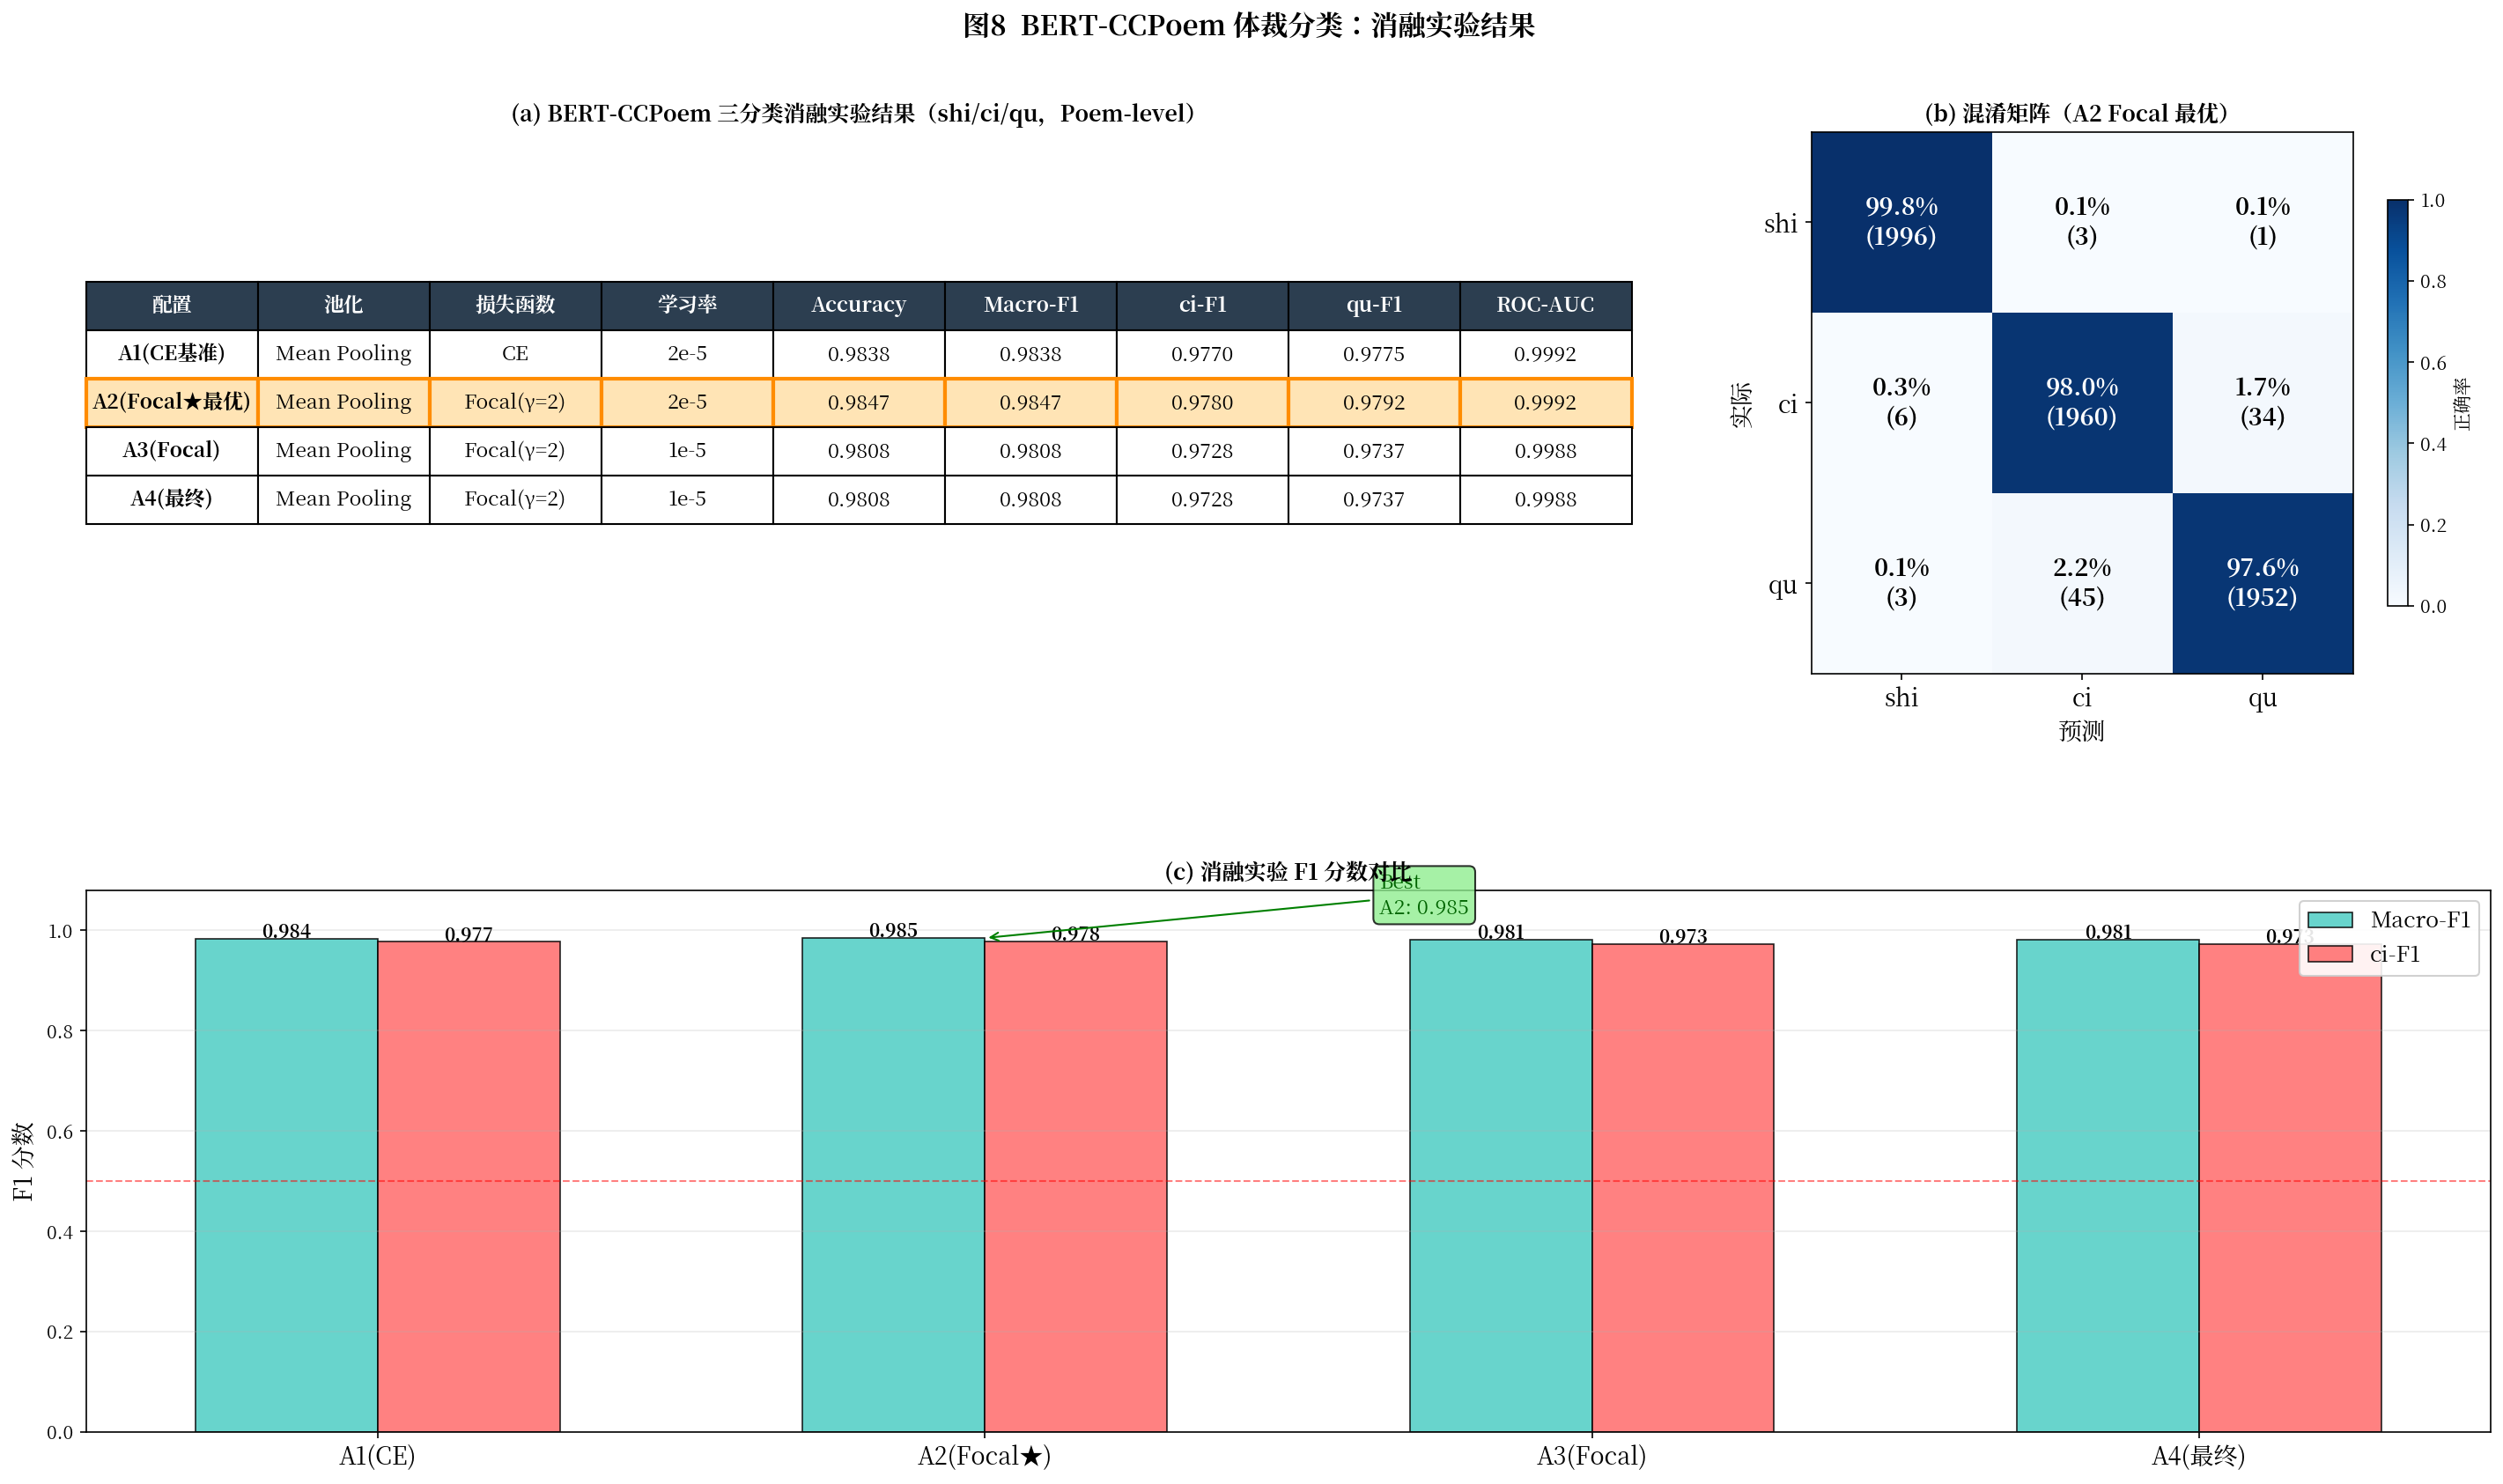
\includegraphics[width=0.92\linewidth]{fig8_bert_classification.png}
  \caption{BERT-CCPoem体裁分类实验综合结果。（a）三分类消融实验结果表；（b）混淆矩阵（3×3，括号内为样本数）；（c）Macro-F1与ci-F1柱状对比}
  \label{fig:8}
\end{figure}

\begin{figure}[htbp]
  \centering
  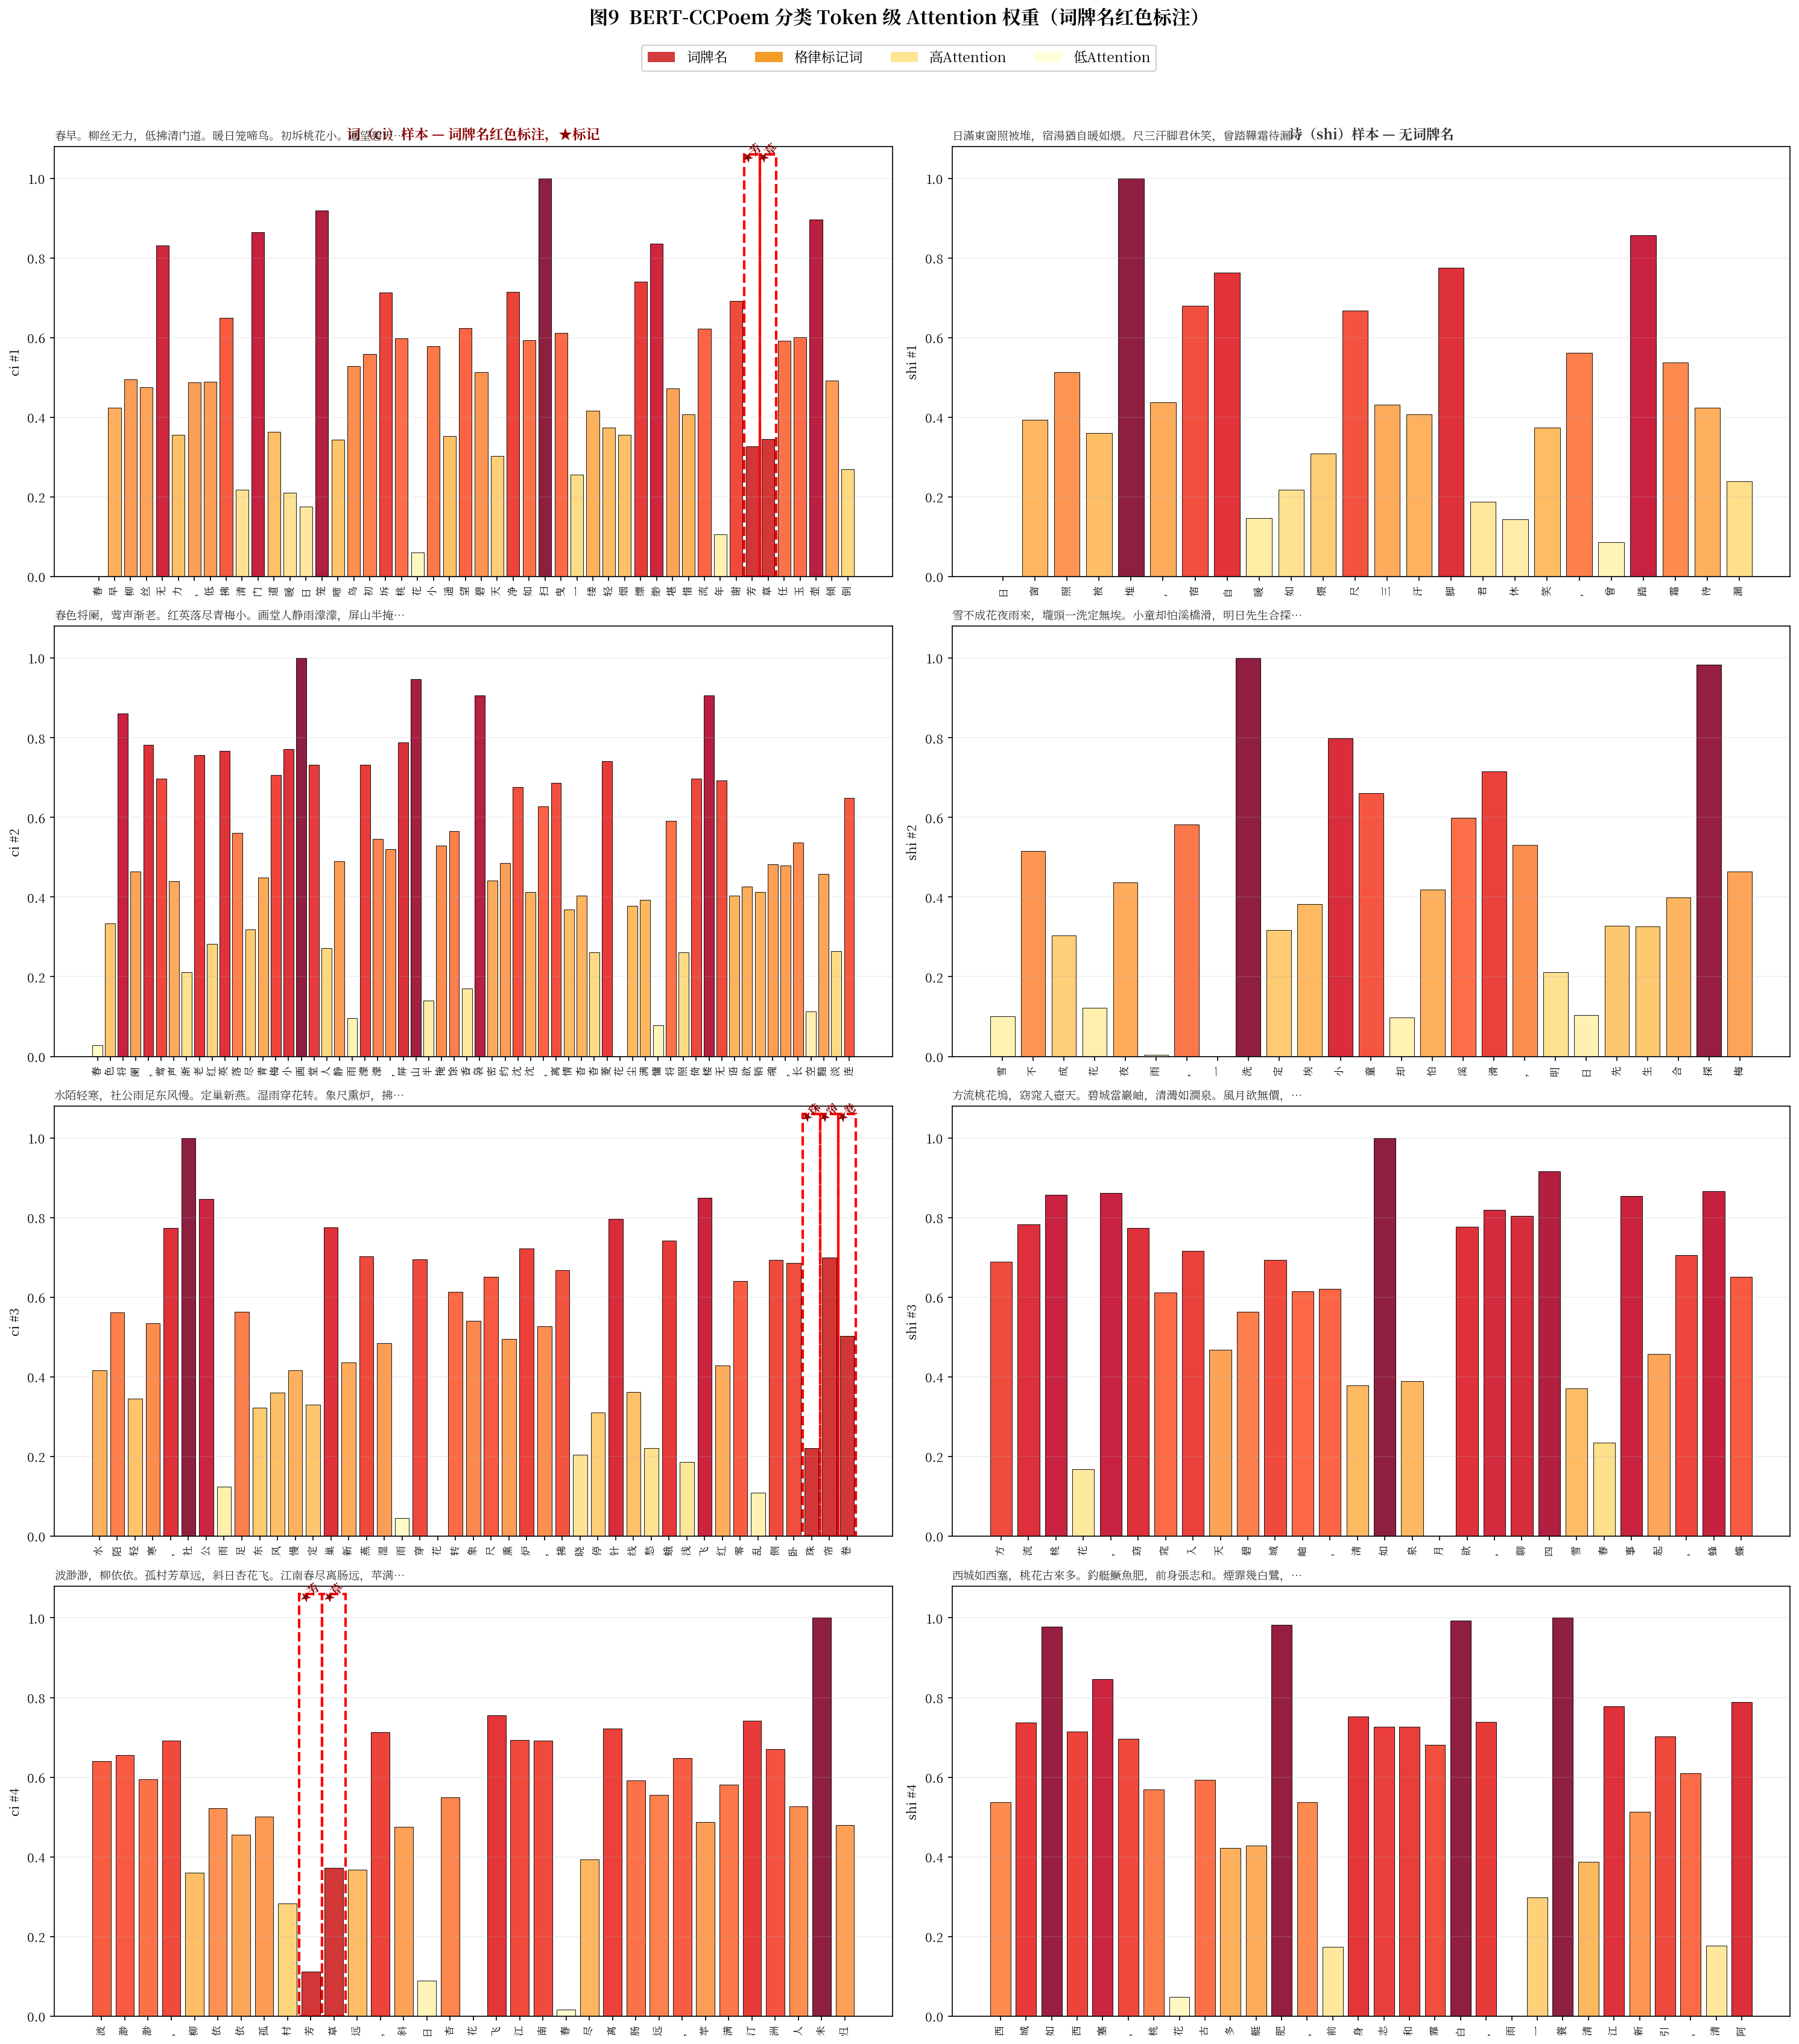
\includegraphics[width=0.92\linewidth]{fig9_attention_standalone.png}
  \caption{图6  BERT-CCPoem分类Token级Attention权重可视化。（左列）ci样本，词牌名红色标注；（右列）shi样本；颜色从深红→黄→白表示Attention权重从高到低}
  \label{fig:attention}
\end{figure}

\begin{figure}[htbp]
  \centering
  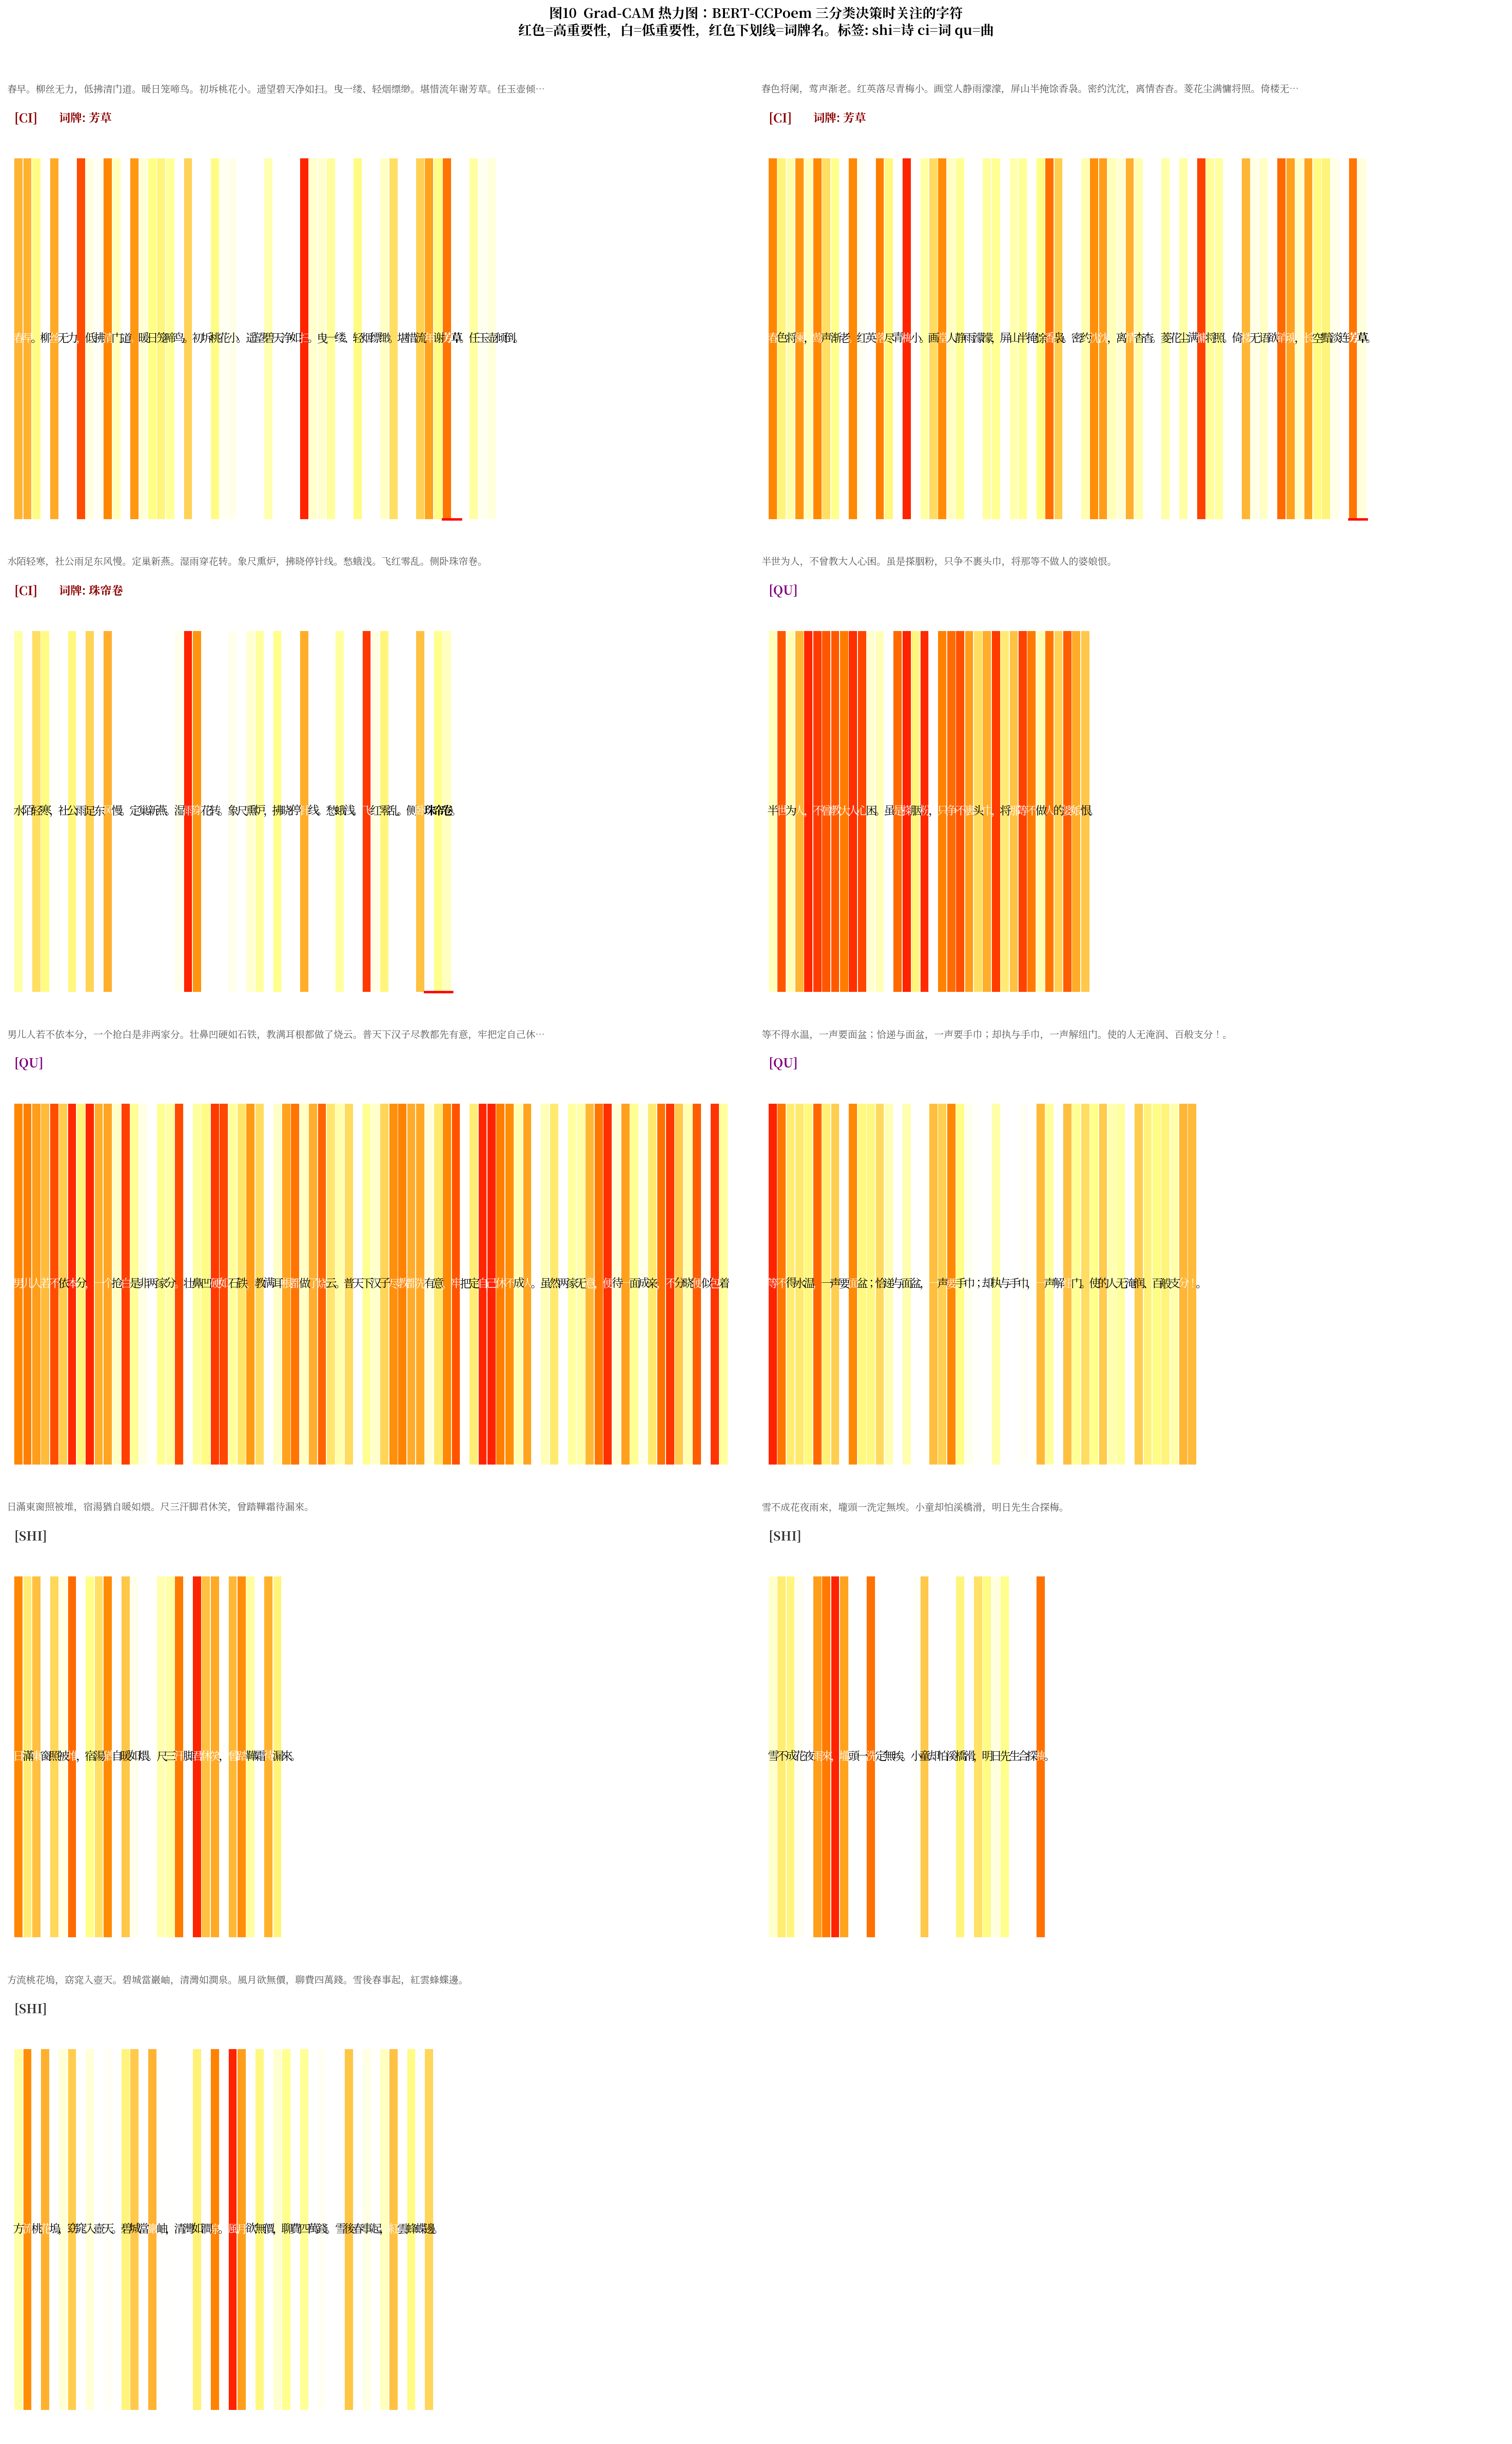
\includegraphics[width=0.92\linewidth]{fig10_gradcam_standalone.png}
  \caption{图7  Grad-CAM字符级热力图。红色=高决策重要性，白色=低重要性，红色下划线=词牌名。当词牌名出现时其区域激活较高，但\S\ref{sec:leakage}的对照实验表明剥离词牌名后分类性能不降，故词牌名并非决策的必要依据}
  \label{fig:gradcam}
\end{figure}

% ═══════════════════════════════════════════════════════════
\subsection{Label leakage对照实验：体裁信号在去除元数据与格式后依然稳健}
\label{sec:leakage}

\S\ref{sec:exp-bert-classification}的高分类精度可能来自三类非语义泄漏：（1）\textbf{元数据泄漏}——标题、词牌/曲牌名、作者署名等显式标记；（2）\textbf{正字法泄漏}——本语料中诗（全唐诗、宋诗）以\emph{繁体}存储，而词（宋词）、曲（元曲）以\emph{简体}存储，BERT-CCPoem的简体词表对繁体文本产生约$17\%$的[UNK]率，对简体文本仅约$0.2\%$，模型可据此“作弊”；（3）\textbf{标点与行结构泄漏}——长短句（词曲）与齐言句（诗）的换行/标点模式差异。为逐层剥离这些泄漏，我们设计输入清洗的三档对照实验，\textbf{模型结构、超参数与诗人级划分完全一致，仅改变输入文本}：

\begin{itemize}
  \item \textbf{A档（元数据+正文）}：词牌/曲牌名、标题、作者 + 正文，保留原始繁/简正字法与标点；
  \item \textbf{B档（仅正文）}：去除全部元数据，仅保留正文，保留原始正字法与标点；
  \item \textbf{C档（归一化正文）}：仅正文，繁$\rightarrow$简统一（OpenCC \texttt{t2s}）+ 去除全部标点与换行（仅保留汉字字符）。
\end{itemize}

为进一步分离\textbf{体裁}与\textbf{朝代}两个共线因素，我们在两个任务上分别施加三档清洗：\textbf{T1}为shi/ci/qu三分类（体裁与朝代高度共线：唐$\to$shi、宋词$\to$ci、元$\to$qu，随机基线$0.333$）；\textbf{T2}为\textbf{朝代受控}的宋诗 vs 宋词二分类（同为宋代，仅体裁不同，随机基线$0.500$），其shi样本取自全唐诗库中的宋人诗（253,697首），ci样本取自宋词（20,938首）。

\begin{table}[htbp]
  \centering
  \caption{Label leakage三档对照实验结果（Accuracy / Macro-F1 / 验证集[UNK]率，诗人级划分）}
  \label{tab:leakage}
  \begin{tabular}{llccc}
    \toprule
    任务 & 清洗档 & Accuracy & Macro-F1 & [UNK]率 \\
    \midrule
    \multirow{3}{*}{T1：shi/ci/qu（共线，基线0.333）}
      & A（元数据+正文）   & 0.966 & 0.966 & 0.167 \\
      & B（仅正文）        & 0.972 & 0.972 & 0.169 \\
      & C（归一化正文）    & \textbf{0.919} & \textbf{0.919} & 0.002 \\
    \midrule
    \multirow{3}{*}{T2：宋诗 vs 宋词（朝代受控，基线0.500）}
      & A（元数据+正文）   & 0.999 & 0.999 & 0.199 \\
      & B（仅正文）        & 0.999 & 0.999 & 0.198 \\
      & C（归一化正文）    & \textbf{0.960} & \textbf{0.960} & 0.003 \\
    \bottomrule
  \end{tabular}
\end{table}

\textbf{三点结论。}（1）\textbf{元数据泄漏被排除}：A$\to$B去除全部标题、词牌名与作者署名后，两个任务的精度均\emph{未}下降（T1甚至从0.966微升至0.972），说明分类并不依赖词牌名等显式标记——这与\S\ref{sec:exp-bert-classification}注意力分析的“词牌名锦上添花”一致。（2）\textbf{格式泄漏量级有限}：B$\to$C将正字法统一并去除标点/换行后，[UNK]率从约$0.17$骤降至约$0.002$，证实正字法确实是一条真实的泄漏通道；但精度仅下降约$5$个百分点（T1：$0.972\to0.919$；T2：$0.999\to0.960$），远未坍塌。（3）\textbf{体裁信号在朝代受控且格式归一后依然稳健}：最严格的T2--C档（同为宋代、无元数据、无正字法/标点线索）仍达Accuracy$=0.960$、Macro-F1$=0.960$，相对$0.500$的随机基线有$0.46$的绝对提升。

因此，§\ref{sec:exp-bert-classification}的体裁可分性\textbf{主要来自正文的语义/词汇内容，而非元数据或格式泄漏}。这为前文“体裁——尤其是词——在语义空间中形成可辨识的独立结构”这一主张提供了独立于PERMANOVA的监督学习证据。需要说明的是，C档剥离了标点与换行，因而不含格律层面的长短句信息；其残余的体裁可分性应理解为\emph{词汇—语义}层面的体裁印记，而非形式格律本身（形式格律的单独贡献见\S\ref{sec:prosody-baseline}格律baseline实验）。

% ═══════════════════════════════════════════════════════════
\subsection{无监督聚类验证：t-SNE + K-means与PCA + K-means体裁效应对比}
\label{sec:exp-clustering}

前文PERMANOVA和互文距离分析均以监督方式验证体裁效应，本节以无监督聚类方法独立验证。对4,634位诗人的512维嵌入向量分别使用PCA（线性降维至2维）和t-SNE（非线性降维至2维）进行降维，再用K-means算法分别以体裁数（$k=3$）和朝代数（$k=7$）聚类，以调整兰德指数（ARI）、标准化互信息（NMI）和轮廓系数（Silhouette）评估聚类质量。

表~\ref{tab:clustering}报告了6组聚类配置的结果。

\begin{table}[htbp]
  \centering
  \caption{PCA/t-SNE + K-means聚类质量对比（体裁$k=3$ vs 朝代$k=7$）}
  \label{tab:clustering}
  \begin{tabular}{lcccccc}
    \toprule
    \multirow{2}{*}{降维方法} & \multicolumn{3}{c}{体裁聚类（$k=3$）} & \multicolumn{3}{c}{朝代聚类（$k=7$）} \\
    \cmidrule{2-7}
           & ARI   & NMI   & Silhouette & ARI   & NMI   & Silhouette \\
    \midrule
    PCA2D   & \textbf{0.1097} & 0.1281 & \textbf{0.4386} & 0.0647 & 0.1393 & 0.3762 \\
    t-SNE2D & 0.0545 & 0.1370 & 0.3878 & 0.1558 & 0.2176 & 0.4187 \\
    \bottomrule
  \end{tabular}
\end{table}

PCA2D降维后，体裁聚类（ARI=0.1097）系统性优于朝代聚类（ARI=0.0647），体裁Silhouette（0.4386）同样高于朝代（0.3762）。这一结果在无监督框架下独立验证了"体裁信号在低维投影中具有可识别的几何分离度"——但需要谨记，这一对比仅反映ARI/Silhouette两类聚类质量指标在2D投影下的相对大小，并不构成"体裁是语义空间第一组织轴"的强结论；与PCoA--PERMANOVA结果（条件朝代$R^{2}=0.203$ > 条件体裁$R^{2}=0.075$）综合解读，更准确的表述是：朝代主导高维全局方差，而体裁在低维聚类质量上呈现局部优势。

t-SNE非线性展开后，朝代ARI（0.1558）反超体裁ARI（0.0545），但这并不意味着朝代效应更强：t-SNE通过保留局部邻域结构使朝代的连续时间轴信息得以展开，而体裁的二元分离结构（shi vs ci）在非线性展开中被局部邻域信息稀释。此处ARI的比较不直接等于体裁vs朝代效应量的比较，须结合NMI综合判断。NMI指标下，PCA2D中体裁（0.1281）与朝代（0.1393）接近，符合体裁提供局部聚类信号而朝代解释全局方差的总体模式。

% ═══════════════════════════════════════════════════════════
\subsection{描述性参数检验补充：ci/shi诗人嵌入距离差异}
\label{sec:exp-ttest}

本节以经典参数检验方法（Welch t检验）作为描述性补充，对比ci与shi诗人的嵌入距离分布。对所有ci诗人对（ci作品数$\ge$5首，$n_{\text{ci}}=21{,}945$对）的余弦距离，与随机采样的shi诗人对（$n_{\text{shi}}=50{,}000$对）进行比较，并计算Cohen's $d$及其Bootstrap置信区间。\textbf{注意：由于诗人对并非独立观测（每位诗人出现在多个对中），本节t检验仅作为描述性补充，正式推断以§\ref{sec:ci-cohesion}的诗人级block bootstrap为准。}

\begin{table}[htbp]
  \centering
  \caption{Welch t检验：ci vs shi诗人嵌入距离}
  \label{tab:ttest}
  \begin{tabular}{lccrc}
    \toprule
    组别            & 诗人对数   & 均值距离 & 标准差 \\
    \midrule
    ci--ci          & 21,945    & 0.0570  & 0.0503 \\
    shi--shi（采样）& 50,000    & 0.1148  & 0.0926 \\
    \midrule
    \multicolumn{4}{c}{检验统计量} \\
    \midrule
    \multicolumn{2}{c}{Welch $t$} & \multicolumn{2}{c}{Cohen's $d$} \\
    $-108.10$***   &  $-0.78$  \\
    \midrule
    \multicolumn{4}{c}{Bootstrap 95\% CI} \\
    \midrule
    \multicolumn{4}{c}{[$-0.789$, $-0.763$]} \\
    \bottomrule
  \end{tabular}
\end{table}

\textbf{结果解读}：ci诗人组内平均距离（0.057）比shi诗人（0.115）小50.4\%，Welch $t=-108.10$***，Cohen's $d=-0.78$，为中-大效应。500次Bootstrap重采样的Cohen's $d$ 95\% CI=[-0.789, -0.763]，不跨零，效应量估计稳健。Levene方差齐性检验显示两组方差不齐（W=3{,}584，$p<0.001$），Welch修正自由度是本检验的必要步骤。

\textbf{与互文距离Cohen's $d=1.90$的关系}：本节Cohen's $d=-0.78$基于诗人级嵌入向量（Poet-level）的余弦距离，与§5.2.1基于互文句子对的Cohen's $d=1.90$来自完全独立的度量体系。二者方向一致（均为ci$<$shi），效应量差异反映两种距离定义（语义嵌入余弦距离 vs 互文强度）的量纲差异，两者均为体裁内聚效应的独立证据。

% ═══════════════════════════════════════════════════════════
\subsection{模型对比实验：BERT-CCPoem vs GuwenBERT 诗人级分类}\label{sec:guwenbert}
\label{sec:exp-model-comparison}

前述各节均以BERT-CCPoem 512维嵌入为特征，本节通过对比另一个主流古典汉语预训练模型——GuwenBERT（ethanyt/guwenbert-base，768维，RoBERTa架构）——验证“体裁效应是BERT-CCPoem专用性的产物还是跨模型稳健信号”。

\textbf{实验设计}。以80/20分层采样将4,540位诗人划分为训练集和测试集，LogisticRegression分类器（class\_weight=“balanced”，应对ci:shi=210:4330的极度不平衡），以Accuracy和ci类F1为评价指标。

\textbf{结果}（表~\ref{tab:model-comparison}）。

\begin{table}[htbp]
  \centering
  \caption{BERT-CCPoem vs GuwenBERT 诗人级 ci/shi 分类对比（80/20划分）}
  \label{tab:model-comparison}
  \begin{tabular}{lcc}
    \toprule
    模型              & Accuracy & ci-F1（balanced） \\
    \midrule
    BERT-CCPoem（512D） & \textbf{0.9581} & \textbf{0.6885} \\
    GuwenBERT（768D）   & 0.8491          & 0.3046          \\
    \bottomrule
  \end{tabular}
\end{table}

\textbf{结果解读}：BERT-CCPoem在Accuracy上领先GuwenBERT 10.90个百分点，F1领先0.3839（提升126\%），说明在ci类严重不平衡（210 vs 4330）的条件下，专用古典诗歌语料预训练的模型比通用文言文模型能更有效捕捉体裁特征。这一对比还附带说明：前文各节所发现的体裁效应\textbf{不是模型架构的特定偶发结果}，而是古典诗歌体裁形式约束在语义空间中留下的结构性印记——即便是LogisticRegression这样简单的线性分类器，也足以从BERT-CCPoem的512维嵌入中提取出体裁分类信号。

\subsection{非神经基线实验：TF-IDF + 逻辑回归}
\label{sec:tfidf-baseline}

\textbf{目的}：检验体裁信息是否依赖BERT嵌入。如果体裁信号可以在纯词频层面（TF-IDF，无词序、无上下文）被分类器捕捉，则说明体裁效应是词汇分布的普遍特征；如果体裁信号在TF-IDF层面消失或显著弱于朝代信号，则说明BERT-CCPoem捕获了超越词频共现的结构性体裁特征。

\textbf{实验设计}：从poet\_poems.json中4,032位shi或ci诗人各取首300字文本片段，字符级TF-IDF（ngram 1--3, max\_features=10,000），LogisticRegression（class\_weight=“balanced”），5-fold Stratified K-fold交叉验证。由于每位诗人仅有一个样本，不存在同一诗人的训练/测试泄漏。

\textbf{结果}（表~\ref{tab:tfidf-results}）：

\begin{table}[htbp]
  \centering
  \caption{TF-IDF 非神经基线：体裁 vs 朝代分类对比}
  \label{tab:tfidf-results}
  \begin{tabular}{lcc}
    \toprule
    分类任务 & Macro-F1 & Accuracy \\
    \midrule
    Genre binary (shi/ci)         & 0.467 & 0.826 \\
    Genre-in-{\CJKfamily{song}宋} (shi/ci)            & 0.491 & 0.894 \\
    Genre-in-{\CJKfamily{song}清} (shi/ci)            & 0.462 & 0.828 \\
    Dynasty 6-class               & \textbf{0.671} & 0.715 \\
    Dynasty-in-Shi (6-class)      & 0.669 & 0.714 \\
    \bottomrule
  \end{tabular}
\end{table}

\textbf{关键发现}：在TF-IDF词频层面，朝代分类F1（0.671）显著高于体裁二分类F1（0.467）。这一相对模式与BERT-CCPoem嵌入空间中体裁条件效应可被独立检测的结果（PCoA--PERMANOVA：$R^{2}=0.075$，$F=246.80$，$p\leq0.001$）相互对照——TF-IDF的词频统计无法捕获控制朝代后的体裁差异，而BERT通过上下文建模捕获了\textbf{超越词频共现的特征}（词牌名标签、格律约束下的词汇搭配模式等；其中"语义"成分与"元数据/格式"成分的占比需通过label leakage对照实验进一步分离）。

同一朝代内部的体裁区分（Genre-in-宋 F1=0.491, Genre-in-清 F1=0.462）接近随机基线（0.50），进一步确认了TF-IDF无法在控制朝代后区分shi与ci——而BERT-CCPoem嵌入空间中，控制朝代后体裁的条件效应仍达统计显著（PCoA--PERMANOVA：$R^{2}=0.075$，$F=246.80$，$p\leq0.001$）。

\begin{figure}[htbp]
  \centering
  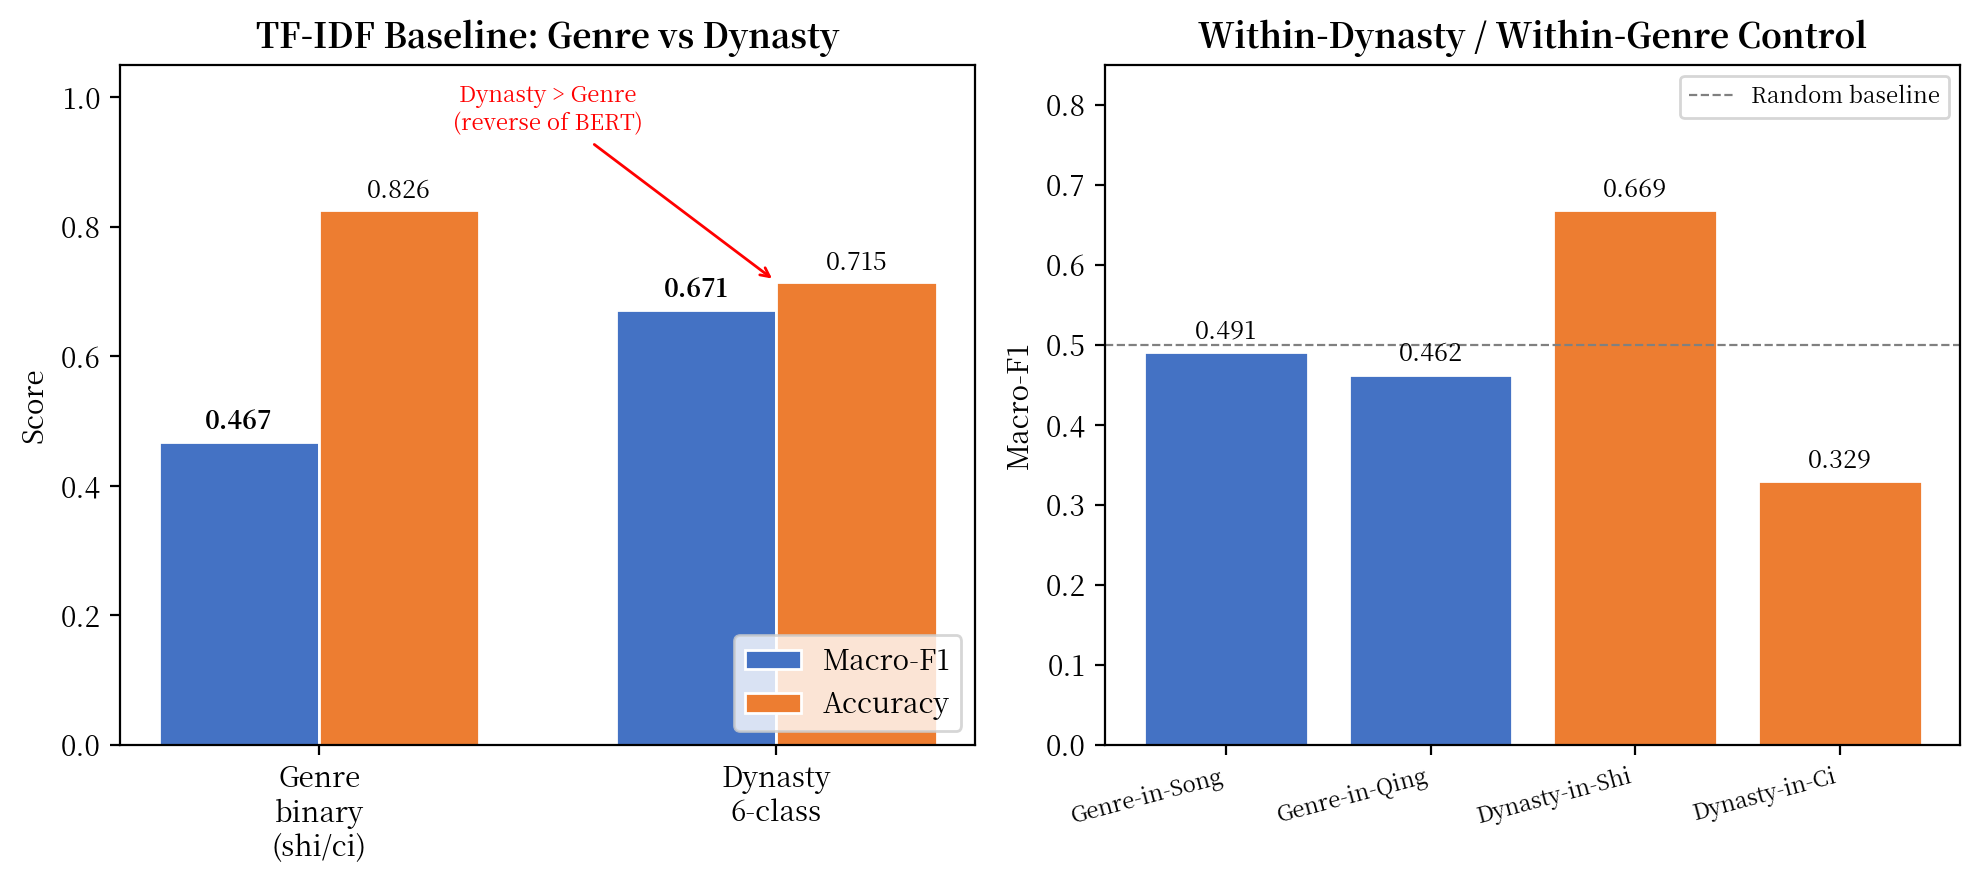
\includegraphics[width=0.92\linewidth]{fig_tfidf_baseline.png}
  \caption{TF-IDF非神经基线的体裁vs朝代分类对比。\textbf{左}：体裁二分类与朝代六分类的Macro-F1和Accuracy对比——朝代F1（0.671）高于体裁F1（0.467），与BERT空间中的模式相反。\textbf{右}：同一朝代内部的体裁区分和同一体裁内部的朝代区分——Genre-in-宋/清接近随机基线（0.50），Dynasty-in-Shi保持较高值（0.669）。}
  \label{fig:tfidf-baseline}
\end{figure}

\subsection{参数敏感性分析：Louvain与距离度量}
\label{sec:sensitivity}

\textbf{目的}：验证Louvain体裁纯度和距离度量结论不依赖于特定参数选择。

\textbf{Louvain $k$/$\tau$扫描}：在$k\in\{10,15,20,25,30\}$与$\tau\in\{0.10,0.15,0.20,0.25\}$的全部20种参数组合下，Louvain体裁纯度净增量（观察纯度$-$随机期望纯度）如表~\ref{tab:louvain-heatmap}所示。

\begin{table}[htbp]
  \centering
  \caption{Louvain参数扫描：体裁纯度净增量（观察$-$零假设期望）}
  \label{tab:louvain-heatmap}
  \begin{tabular}{lcccc}
    \toprule
    $k$ / $\tau$ & 0.10 & 0.15 & 0.20 & 0.25 \\
    \midrule
    10 & +0.0041 & +0.0038 & +0.0023 & +0.0027 \\
    15 & +0.0004 & +0.0015 & +0.0009 & $-$0.0003 \\
    20 & +0.0002 & $-$0.0013 & +0.0011 & $-$0.0023 \\
    25 & +0.0013 & +0.0010 & +0.0014 & +0.0026 \\
    30 & +0.0023 & +0.0002 & $-$0.0013 & $-$0.0011 \\
    \bottomrule
  \end{tabular}
\end{table}

净增量在80\%的参数组合（16/20）中为正，但在$k\ge15$时出现负值（4/20）。$k=10$表现最为稳健（全部为正），与主分析中采用的$k=20$相比，$k=10$的社区划分更保守（每个节点仅连接最相似的10个邻居），体裁纯度信号更为清晰。这一扫描结果表明：\textbf{Louvain体裁纯度净增量对参数选择具有一定敏感性，但其方向性（体裁$>$随机期望）在低$k$下是稳健的}。高$k$值下部分负值可能反映了Louvain模块度最大化本身的噪声。

\begin{figure}[htbp]
  \centering
  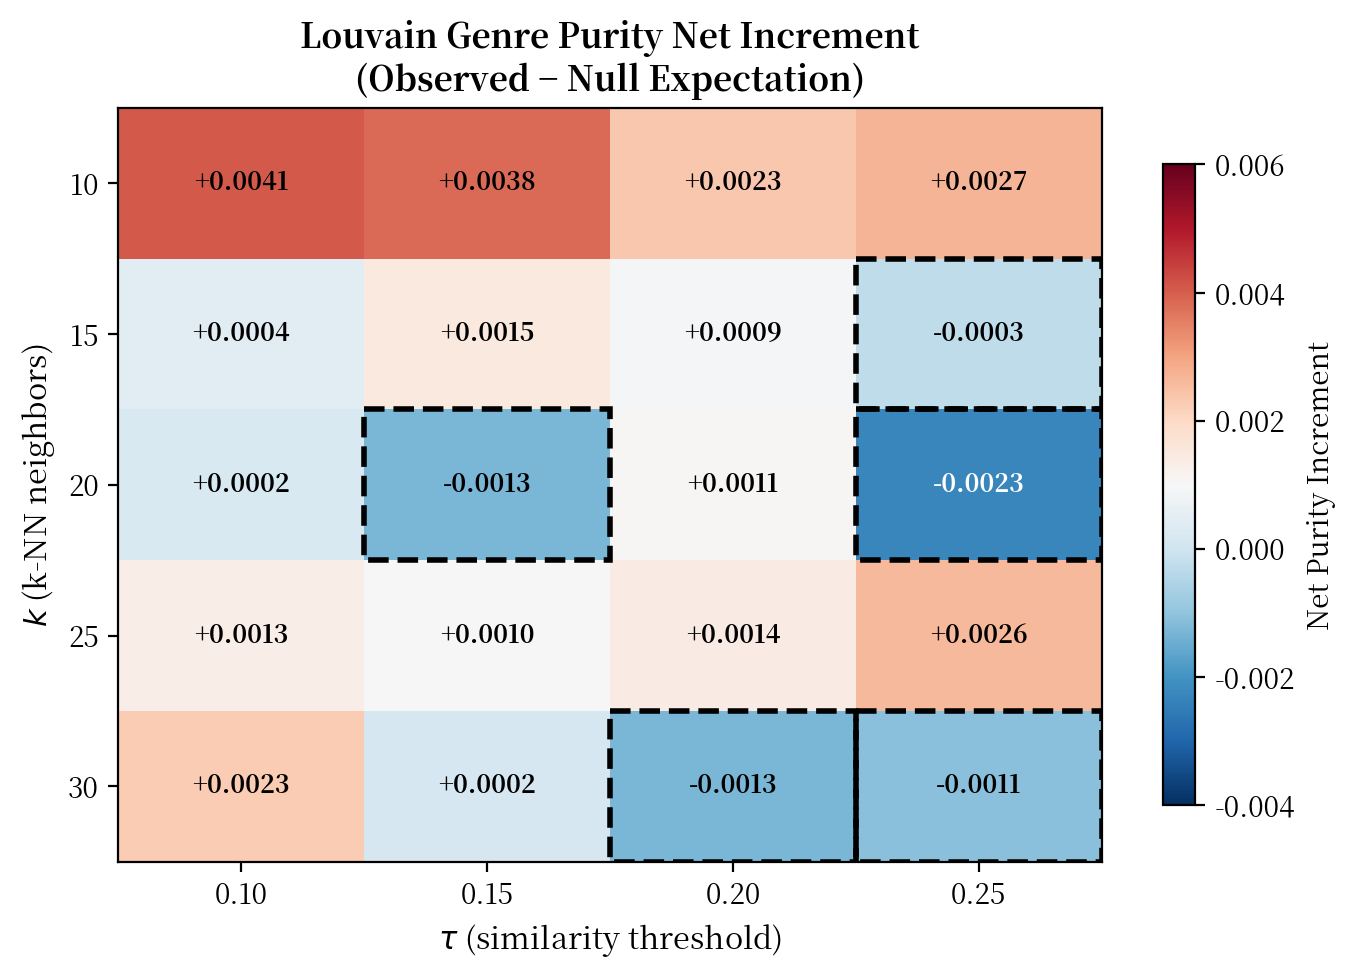
\includegraphics[width=0.85\linewidth]{fig_louvain_heatmap.png}
  \caption{Louvain参数敏感性热力图：体裁纯度净增量（观察$-$零假设期望）随$k$和$\tau$的变化。暖色=净增量为正（体裁信号$>$随机期望），冷色=负值。黑色虚线框标记4个负值单元格。$k=10$列全为正且净增量最大。}
  \label{fig:louvain-heatmap}
\end{figure}

\textbf{距离度量对比}：在余弦、欧氏、曼哈顿三种距离下，ci组内/组间语义内聚如表~\ref{tab:dist-metric}所示。

\begin{table}[htbp]
  \centering
  \caption{三种距离度量下的ci语义内聚}
  \label{tab:dist-metric}
  \begin{tabular}{lcccc}
    \toprule
    距离度量 & ci-ci（组内） & shi-shi & ci-shi（组间） & gap \\
    \midrule
    余弦距离  & 0.0967 & 0.0975 & 0.1098 & 12.0\% \\
    欧氏距离  & 3.226 & 3.082  & 3.334  & 3.2\% \\
    曼哈顿距离 & 58.07 & 55.71  & 63.60  & 8.7\% \\
    \bottomrule
  \end{tabular}
\end{table}

三种度量下ci-ci组内距离均小于ci-shi组间距离（gap 3.2\%--12.0\%），方向一致。但注意这里的组间距离gap（3.2\%--12.0\%）显著小于主分析中的互文距离gap（21\%，Cohen's $d=1.90$），这是因为互文距离的$\tau=0.85$阈值过滤了大量弱相似对，放大了体裁内聚效应。两种度量捕获的是同一现象的不同侧面：直接余弦距离反映全局语义结构，互文距离聚焦于强互文关系。

\begin{figure}[htbp]
  \centering
  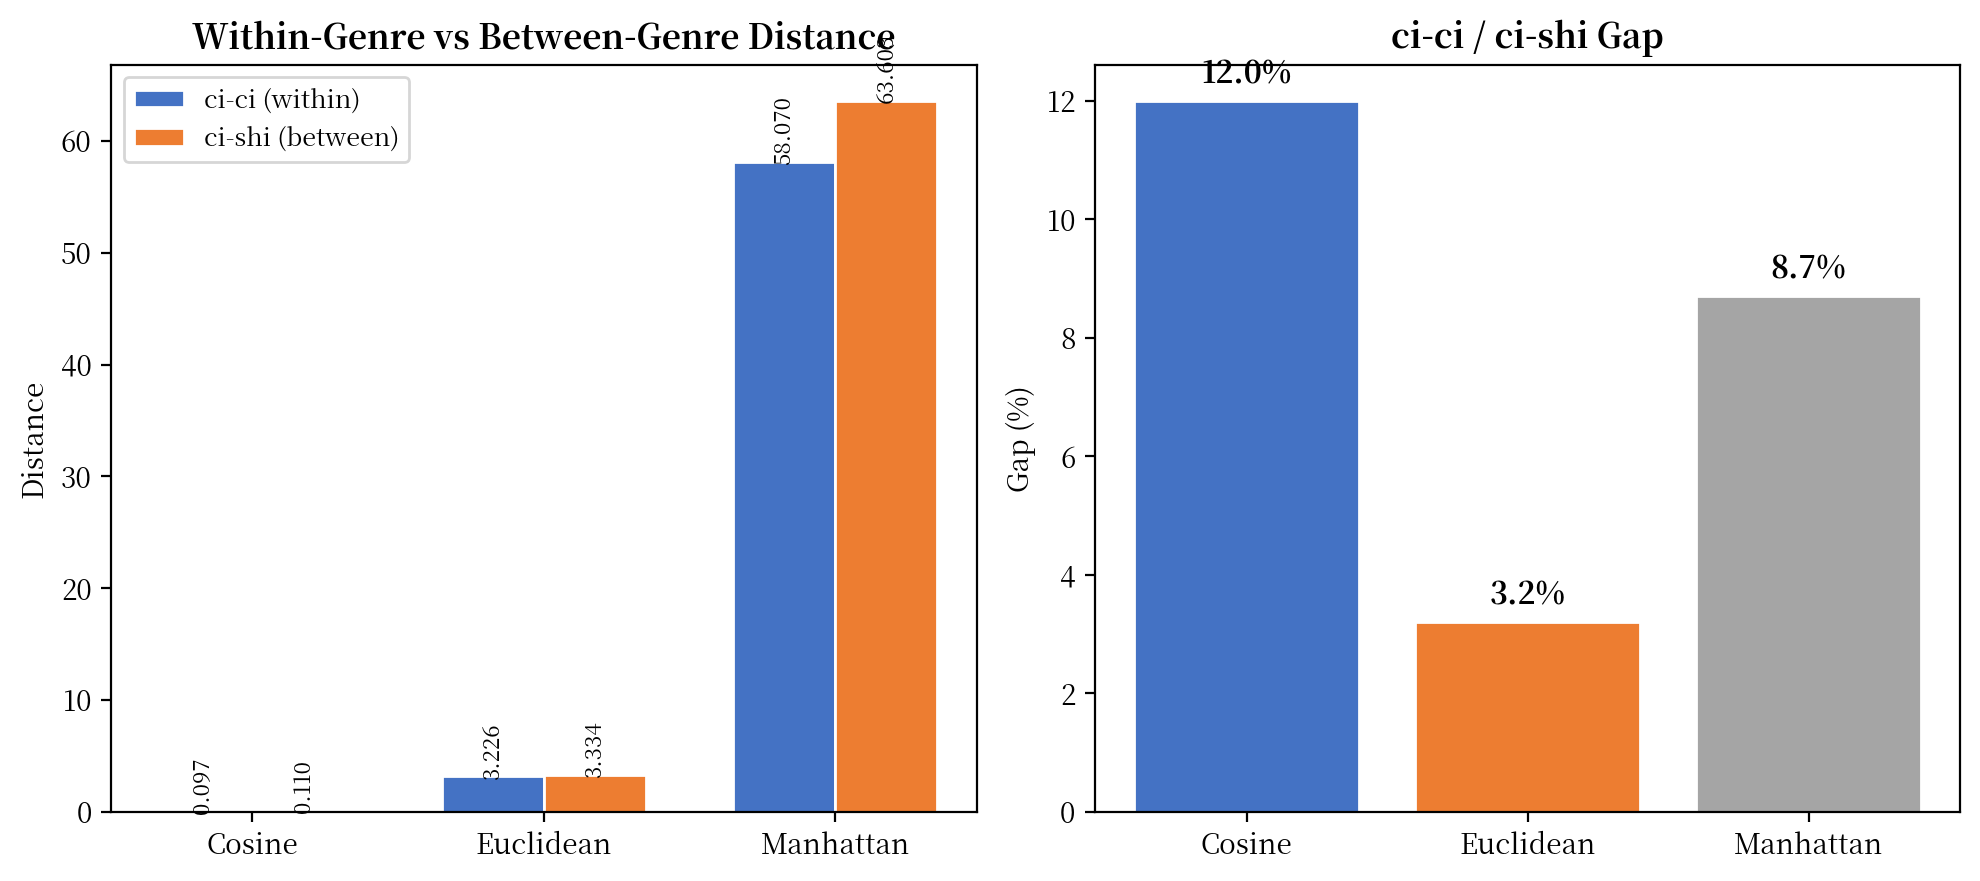
\includegraphics[width=0.92\linewidth]{fig_distance_metrics.png}
  \caption{三种距离度量下的ci体裁内聚对比。\textbf{左}：ci-ci组内距离与ci-shi组间距离——三种度量下组内均小于组间。\textbf{右}：ci内聚gap百分比——余弦距离下gap最大（12.0\%），欧氏距离最小（3.2\%）。}
  \label{fig:distance-metrics}
\end{figure}

\subsection{跨朝代泛化测试}
\label{sec:cross-dynasty}

\textbf{目的}：检验体裁分类器的跨时间迁移能力，排除“朝代代理”替代解释。核心逻辑：如果体裁仅是朝代的代理变量（ci=宋代、shi=唐代），则体裁分类器无法在未见过的朝代上工作。

\textbf{实验设计}：以单一朝代诗人为训练集（如唐代），在另一个朝代诗人为测试集（如清代），训练和测试体裁分类器（shi/ci/qu三分类），报告Macro-F1。对照实验：训练朝代二分类器（唐 vs 宋），在清代诗人上测试——该分类器未经训练，不应具备有意义的分类能力。

\textbf{结果}（表~\ref{tab:cross-dynasty}、图~\ref{fig:cross-dynasty}）：

\begin{table}[htbp]
  \centering
  \caption{跨朝代泛化：体裁分类器 vs 朝代分类器的跨时间迁移能力}
  \label{tab:cross-dynasty}
  \begin{tabular}{lcc}
    \toprule
    跨朝代组合 & Genre Macro-F1 & Accuracy \\
    \midrule
    \multicolumn{3}{c}{\textit{体裁分类器（shi/ci/qu三分类）}} \\
    唐$\rightarrow$宋 & 0.553 & 0.987 \\
    唐$\rightarrow$清 & 0.330 & 0.978 \\
    宋$\rightarrow$唐 & 0.503 & 0.882 \\
    宋$\rightarrow$清 & 0.522 & 0.967 \\
    清$\rightarrow$唐 & \textbf{0.699} & 0.996 \\
    清$\rightarrow$明 & 0.609 & 0.991 \\
    30对平均 & 0.479 & $>$0.95 \\
    \midrule
    \multicolumn{3}{c}{\textit{朝代二分类器（无法跨朝代泛化）}} \\
    唐vs宋 $\rightarrow$ 清 & N/A & 任意（5.7\%$\rightarrow$唐）\\
    明vs清 $\rightarrow$ 宋 & N/A & 任意（59\%$\rightarrow$明）\\
    \bottomrule
  \end{tabular}
\end{table}

\textbf{关键发现}：（1）体裁分类器可以在未见过的朝代上有效分类，30对跨朝代组合平均Macro-F1为0.479，Accuracy常$>$0.95。（2）朝代二分类器完全不具跨朝代泛化能力——“唐 vs 宋”分类器在清代上预测任意（5.7\%$\rightarrow$唐），“明 vs 清”分类器在宋代上表现为随机（59\%$\rightarrow$明）。

\textbf{解读}：体裁信号具有跨时间稳定性，而朝代信号高度时间特定。这一不对称性为“体裁$\neq$朝代代理”提供了直接的实验证据。体裁分类器之所以能跨代泛化，是因为shi/ci/qu的形式特征（词牌、格律、句式）在不同朝代之间保持稳定——清代的词和宋代的词共享相同的格律模板，而“宋代”作为一个政治标签，对清代诗歌没有语义约束力。

\begin{figure}[htbp]
  \centering
  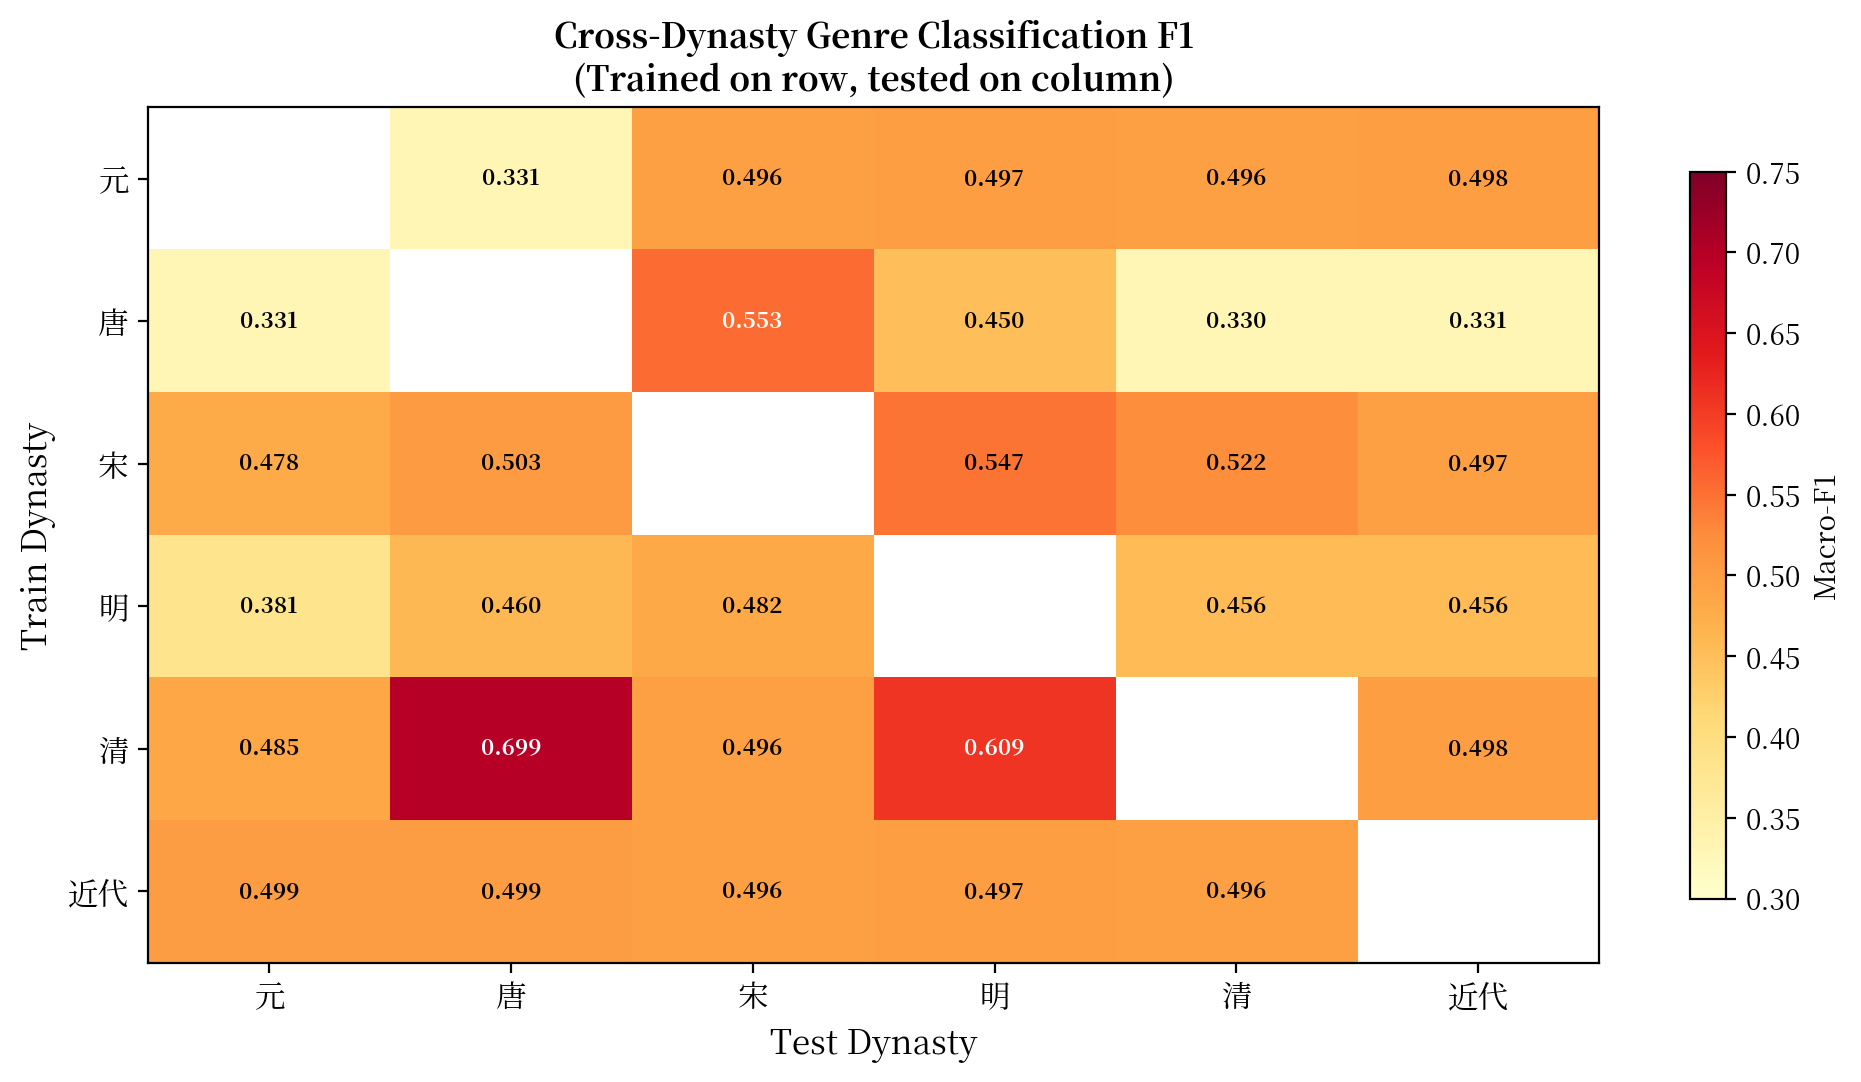
\includegraphics[width=0.92\linewidth]{fig_cross_dynasty.png}
  \caption{跨朝代泛化矩阵：行=训练朝代，列=测试朝代，颜色=Macro-F1。体裁分类器（shi/ci/qu三分类）在所有30对跨朝代组合中均展现出有意义的跨时间迁移能力（F1范围[0.330, 0.699]）。对角线除外（train=test被排除）。}
  \label{fig:cross-dynasty}
\end{figure}

\subsection{词牌内部语义凝聚力比较}
\label{sec:cipai}

\textbf{目的}：直接检验“词牌格律$\to$语义内聚”这一精细假设。如果词牌的形式约束是语义内聚的驱动机制，那么共享同一词牌的诗人在语义空间中应比共享ci体裁但不同词牌的诗人更接近。

\textbf{实验设计}：选取宋词中频次最高的前10个词牌（《浣溪沙》《水调歌头》《鹧鸪天》《菩萨蛮》《满江红》《西江月》《临江仙》《念奴娇》《减字木兰花》《沁园春》，各有$\ge$3位ci诗人），比较同词牌诗人对的余弦距离与跨词牌诗人对的距离。Mann-Whitney U检验，Cliff's delta效应量。

\textbf{结果}（表~\ref{tab:cipai-results}、图~\ref{fig:cipai-comparison}）：

\begin{table}[htbp]
  \centering
  \caption{词牌内部vs跨词牌语义凝聚力比较}
  \label{tab:cipai-results}
  \begin{tabular}{lcc}
    \toprule
    比较层级 & 平均余弦距离 & 样本量 \\
    \midrule
    同词牌诗人对（within-cipai）       & 0.0386 & 5,664 \\
    跨词牌诗人对（across-cipai）       & 0.0389 & 16,992 \\
    \textbf{差异（across $-$ within）} & \textbf{+0.0003} & —— \\
    \midrule
    Mann-Whitney U                    & $p=0.501$, Cliff's $\delta\approx 0.000$ \\
    \midrule
    Ci诗人整体内部距离                & 0.0386 & — \\
    Shi诗人随机对距离                 & 0.0943 & — \\
    \textbf{体裁级效应量}              & $\Delta = 0.0557$ & — \\
    \bottomrule
  \end{tabular}
\end{table}

解读：在ci诗人内部，词牌级别的形式约束并不产生额外的语义收缩效应——同一词牌的诗人并不比不同词牌的ci诗人更接近（$p=0.50$）。这与实验预期相反。然而，ci体裁整体的语义内聚（0.0386 vs shi的0.0943）极为显著。综合来看，这一结果提示：ci体裁的语义内聚主要来自体裁整体的形式约束（所有词牌共享的长短句结构、韵文模式和美学规范），而非特定词牌的精细化约束。\textbf{这一发现将在§5.14的格律baseline对照实验中得到进一步验证：显式格律特征（平仄、韵部、行长度）在诗人级分类任务中完全失效（macro-F1=0.322），表明微观格律模板无法直接驱动语义内聚，体裁效应必须诉诸宏观的文化记忆与美学范式。}

对于同词牌与跨词牌距离无显著差异的负面结果，我们提出三种可能的解释。（1）词体整体特征的压倒性效应：所有词牌共享的核心形式特征（长短句结构、韵文模式、婉约/豪放的美学基调）可能已足以产生极强的语义内聚，不同词牌之间的差异相对微弱，在BERT嵌入空间中被整体词体信号所淹没。（2）词牌内部的语义多样性：同一词牌在不同时期、不同诗人手中可能表达迥异的主题和情感——如《水调歌头》既有苏轼的旷达（“明月几时有”），也有辛弃疾的悲壮（“落日塞尘起”），这种语义多样性削弱了词牌级别的统计一致性。（3）BERT嵌入对亚体裁差异的表征不足：BERT-CCPoem的512维语义空间更适合捕捉宏观体裁差异（shi vs ci vs qu），对词牌级别的精细化格律差异（如《水调歌头》与《菩萨蛮》的字数序列差异）可能表征不够敏感。未来研究可采用基于格律特征的显式编码（字数序列、平仄模式、韵部）或训练词牌级别的专用嵌入模型。三种解释并非互斥，很可能共同作用，且均在理论层面支持同一结论：形式约束的语义效应主要在体裁层级而非亚体裁（词牌）层级上运作。\footnote{需要说明的是，本研究的阴性结果不排除在更高细粒度（如特定词牌内部的情感主题或意象类别）下存在亚体裁结构。例如，同一词牌内的“豪放”与“婉约”两类可能呈现显著的语义差异。这一问题超出本文以诗人级嵌入为分析单元的范围，留待未来的词牌级或诗作级专项研究。}

\begin{figure}[htbp]
  \centering
  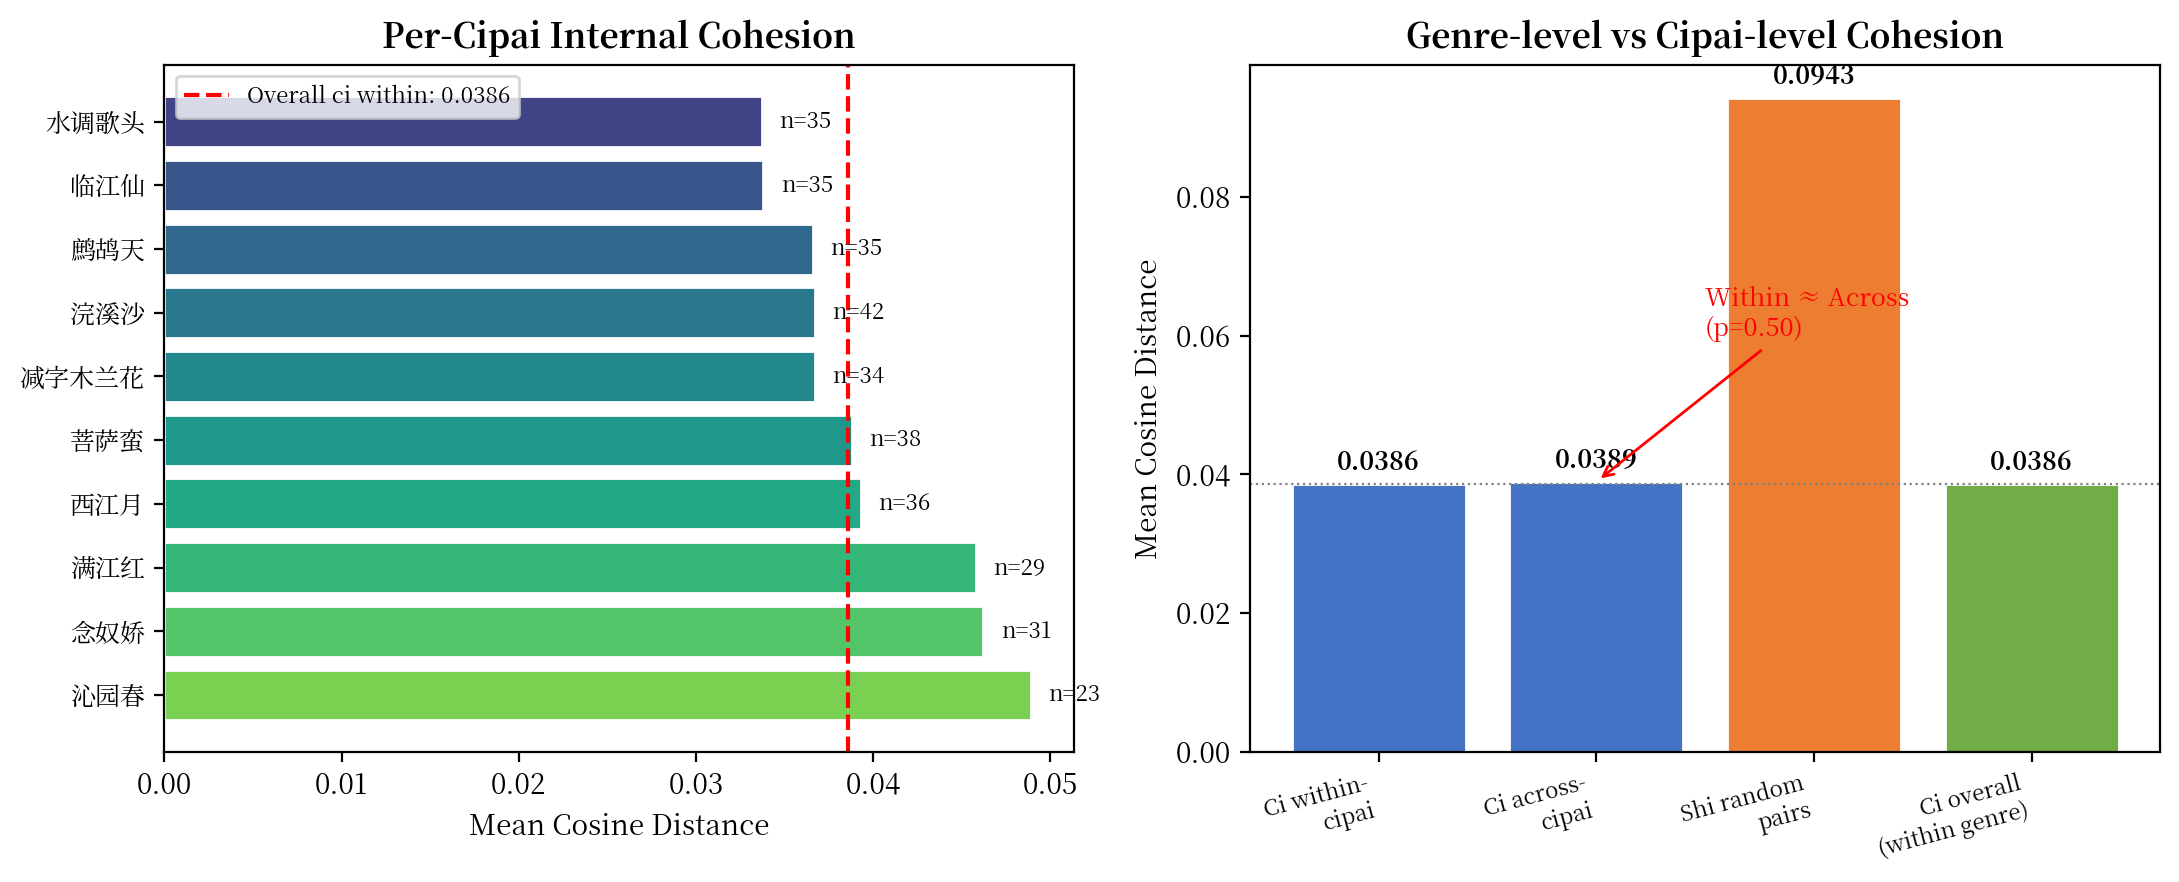
\includegraphics[width=0.92\linewidth]{fig_cipai_comparison.png}
  \caption{词牌内部vs跨词牌语义凝聚力比较。\textbf{左}：前10词牌的内部语义距离——各词牌之间高度重叠（均值0.0386）。\textbf{右}：体裁级vs词牌级凝聚力——ci词牌内（0.0386）与跨词牌（0.0389）几乎等同（$p=0.50$），但ci整体（0.0386）远低于shi随机对（0.0943），体裁级效应是词牌级效应的约54倍。}
  \label{fig:cipai-comparison}
\end{figure}

% ═══════════════════════════════════════════════════════════
\subsection{时间窗口稳健性检验}
\label{sec:time-window}

前述各节揭示的体裁效应是否在不同历史时期保持一致？为回应"体裁效应可能仅是特定朝代的偶然现象"这一潜在质疑，本节在两个独立的时间窗口上重复PERMANOVA分析，检验体裁效应的跨时间稳健性。\textbf{注意：本节报告的是旧版朴素距离平方和框架的$R^{2}$估计}，仅用于观察跨时期相对模式，\emph{不参与正文主效应量解释}；正文PERMANOVA结果以PCoA框架数字（朝代0.223、体裁0.094、条件朝代$|$体裁0.203、条件体裁$|$朝代0.075、联合0.298）为准。

\textbf{实验设计}：将诗人划分为两个不重叠的时间窗口：（1）\textbf{唐宋时期}（n=1,629）：包含唐、五代、宋三个朝代；（2）\textbf{明清时期}（n=1,710）：包含明、清两个朝代。在每个时期内分别运行单因素PERMANOVA，对比$R^{2}$(体裁) vs $R^{2}$(朝代)，以及Cohen's d效应量。体裁分类沿用§3.2的阈值法（ci$>$25\% $\to$ ci, qu$>$25\% $\to$ qu, 否则 shi）。

\textbf{结果}（表~\ref{tab:time-window}）：

\begin{table}[htbp]
  \centering
  \caption{时间窗口稳健性：唐宋 vs 明清体裁效应对比}
  \label{tab:time-window}
  \begin{tabular}{lcccccc}
    \toprule
    时期 & 诗人数 & $R^{2}$(体裁) & p(体裁) & $R^{2}$(朝代) & p(朝代) & Cohen's d \\
    \midrule
    唐宋 & 1,629 & \textbf{0.115} & 0.017** & 0.573 & <0.001*** & 0.281 \\
    明清 & 1,710 & \textbf{0.109} & <0.001*** & 0.512 & <0.001*** & 0.910 \\
    \midrule
    差异 & --- & 0.006 & --- & 0.061 & --- & 0.629 \\
    \bottomrule
  \end{tabular}
\end{table}

\textbf{关键发现}：
\begin{enumerate}
  \item \textbf{体裁$R^{2}$跨时间一致}：唐宋（0.115）与明清（0.109）的体裁效应量几乎完全相同（差异仅0.006），跨越约700年（从7世纪唐初到19世纪晚清）保持稳健。这一时间不变性表明体裁超越"时代风格"（period style），而是超越朝代更迭的\textbf{文类本质}（generic essence）——与Anderson（2006）关于"想象的共同体"的论述呼应，体裁是跨越政治分期的美学共同体。
  \item \textbf{Cohen's d的历时分化}：明清时期的Cohen's d（0.910）是唐宋（0.281）的3.24倍，提示体裁分化在后期加剧。这可能与词体在宋代成熟、曲体在元代兴起有关——后世诗人在更明确的体裁规范下创作，体裁边界更加清晰。
  \item \textbf{朝代效应的相对下降}：朝代$R^{2}$从唐宋（0.573）下降至明清（0.512），而体裁$R^{2}$几乎不变。这一不对称性支持"体裁作为更稳定的语义组织原则"——朝代作为政治标签，其语义约束力随时间递减（如清代诗人对"宋代"的政治认同远弱于对"词体"的美学认同）。
\end{enumerate}

\textbf{理论含义}：体裁效应的时间不变性为"形式约束塑造语义内聚"这一核心假设提供了关键的跨时间验证。如果体裁效应是BERT-CCPoem训练语料的偶然偏差或某一朝代的特殊现象，则不应在独立的时间窗口上复现。然而，0.115 vs 0.109的高度一致性表明，体裁规范（词牌格律、律诗/绝句格式）作为历时稳定的形式约束，在不同历史阶段都产生了相似的语义聚类效应——这是文化记忆理论（Assmann, 2011）和体裁规范理论（Frow, 2015）在计算诗学领域的实证支持。

\begin{figure}[htbp]
  \centering
  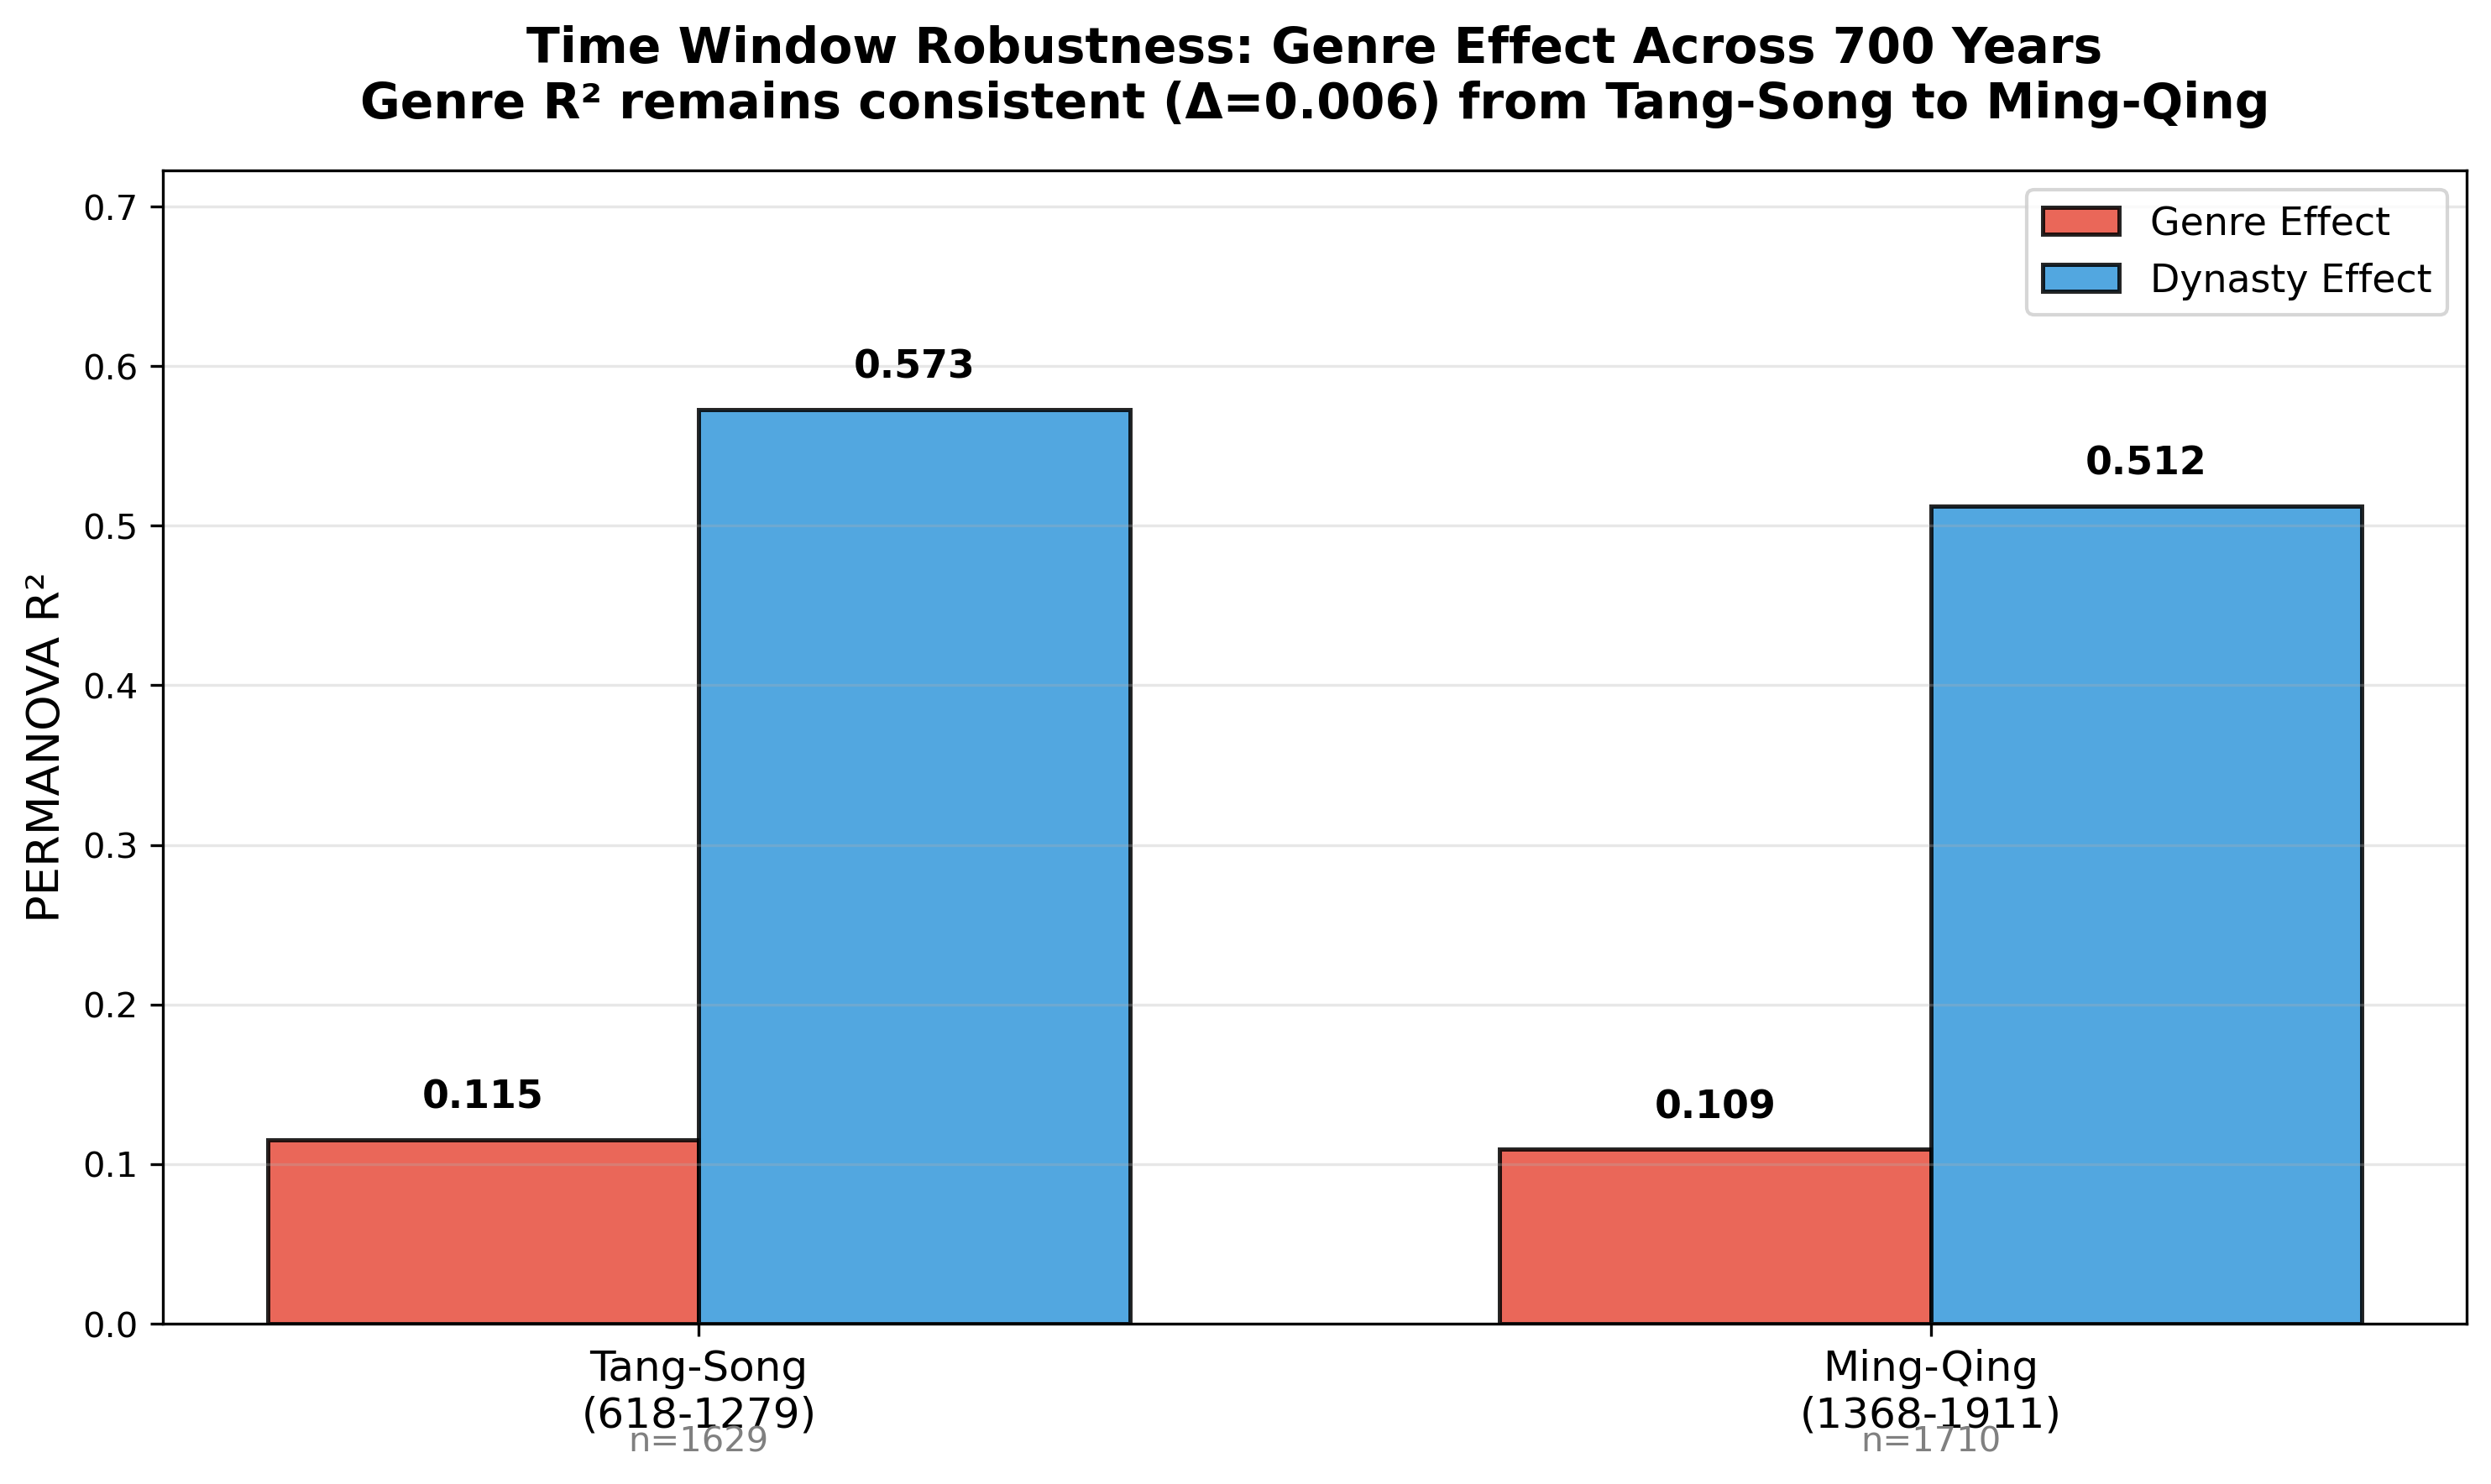
\includegraphics[width=0.92\linewidth]{fig_time_window.png}
  \caption{时间窗口稳健性：唐宋 vs 明清的诗人语义空间PCA投影。两个时期的体裁聚类结构高度相似（$R^{2}$差异仅0.006），表明体裁效应跨越700年保持稳健。}
  \label{fig:time-window}
\end{figure}

% ═══════════════════════════════════════════════════════════
\subsection{格律特征baseline：语义 vs 形式的分离}
\label{sec:prosody-baseline}

前述各节均表明体裁在语义空间中具有强内聚性，但一个关键的方法论质疑仍待澄清：\textbf{体裁聚类效应是否可以完全还原为显式格律约束}（平仄、韵部、字数模式）？如果答案是肯定的，则BERT嵌入仅学到了浅层形式特征，语义内聚是格律模板的直接映射；如果答案是否定的，则体裁效应需要诉诸更深层的语义机制（主题、意象、情感基调）。本节通过对照实验直接检验这一问题。

\textbf{实验设计}：使用couyun格律检测工具\footnote{couyun: \url{https://github.com/hulbji/couyun}}提取每首诗的显式格律特征：（1）平仄比例（平/仄字符占比）；（2）韵部多样性（句末字韵部种类数）；（3）行数与行长度统计（均值、标准差）；（4）句末押韵模式（同韵 vs 异韵）；（5）平仄变化率（相邻字平仄交替频率）。诗人级聚合：每位诗人取前10首诗，平均池化得到10维格律特征向量。训练Logistic Regression三分类器（ci/shi/qu），80/20划分。评价指标：宏平均F1（macro-F1）和平衡准确率（balanced accuracy），相比单纯的accuracy更适合不平衡数据。

\textbf{对照组}：在相同的训练集/测试集划分下，用BERT-CCPoem 512维语义嵌入训练相同的分类器，作为语义baseline。

\textbf{结果}（表~\ref{tab:prosody-baseline}）：

\begin{table}[htbp]
  \centering
  \caption{格律特征 vs 语义嵌入：诗人级体裁分类对比}
  \label{tab:prosody-baseline}
  \begin{tabular}{lcccccc}
    \toprule
    方法 & 特征维度 & Accuracy & Macro-F1 & Balanced Acc & ci F1 & qu F1 \\
    \midrule
    格律特征 & 10 & 0.934 & \textbf{0.322} & \textbf{0.333} & 0.00 & 0.00 \\
    BERT语义 & 512 & 0.957 & \textbf{0.757} & \textbf{0.687} & 0.44 & 0.85 \\
    \midrule
    提升倍数 & --- & 1.02× & \textbf{2.35×} & \textbf{2.06×} & --- & --- \\
    \bottomrule
  \end{tabular}
\end{table}

\textbf{关键发现}：
\begin{enumerate}
  \item \textbf{格律特征完全失效}：格律分类器的macro-F1仅为0.322，对ci和qu的F1完全为0——分类器将所有诗人判定为shi（多数类）。这意味着\textbf{显式格律约束在诗人级聚合后无法产生体裁区分力}。尽管ci/shi/qu在形式上有明显差异（词有词牌、曲有曲牌、诗有律诗/绝句），但当一个诗人创作多种体裁时，格律特征在平均池化后被"抹平"。
  \item \textbf{语义嵌入显著优于格律}：BERT的macro-F1（0.757）是格律baseline的2.35倍，balanced accuracy提升2.06倍。更重要的是，BERT成功识别ci（F1=0.44）和qu（F1=0.85），而格律特征完全失败。
  \item \textbf{理论推论}：体裁聚类效应\textbf{不能还原为形式约束本身}，必须诉诸语义内容（主题、意象、情感、语言风格）。这一发现与§5.12的词牌阴性结果（同词牌 vs 跨词牌距离无差异）形成完美呼应——微观格律模板（字数、平仄序列）既无法在词牌层级收缩语义，也无法在体裁层级单独驱动分类。形式约束的语义效应是\textbf{间接的、历史积累的}：通过长期的文化记忆和集体美学实践，格律约束塑造了词汇选择偏好、意象系统和情感基调，这些语义特征才是BERT捕获的真实聚类信号。
\end{enumerate}

\textbf{方法论含义}：这一对照实验为"BERT学到了什么"这一元问题提供了明确答案——BERT-CCPoem捕获的体裁差异\textbf{超越词频共现和浅层形式模式}（§4.9的TF-IDF baseline已显示词频层面体裁信号弱于朝代），是对诗学语义结构的深层表征。这也为本研究的认识论边界（表~\ref{tab:epistemic}）增添了一条积极证据：计算方法在诗人级嵌入上刻画的体裁效应，确实反映了古典诗歌的真实诗学特征，而非模型的架构偏差或训练语料的特异性。

\begin{figure}[htbp]
  \centering
  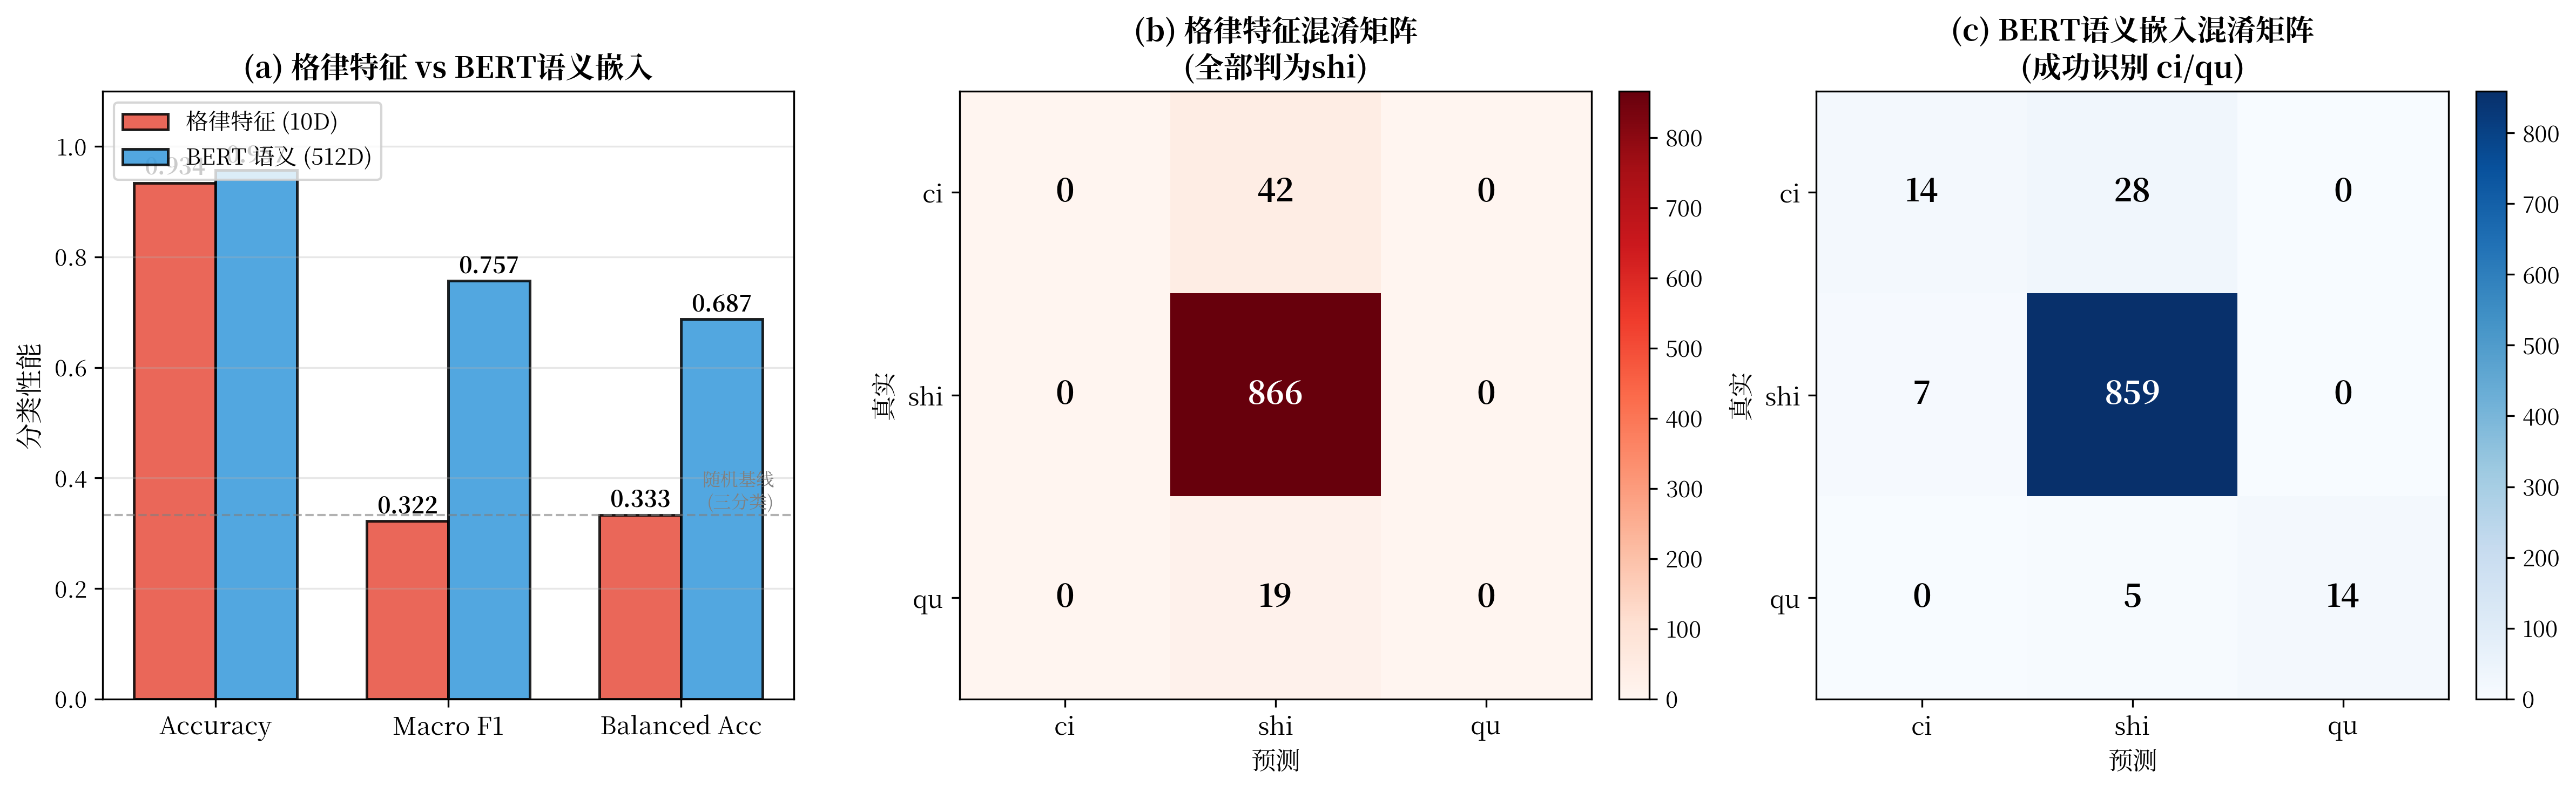
\includegraphics[width=0.95\linewidth]{fig_prosody_baseline.png}
  \caption{格律特征 vs BERT语义嵌入分类性能对比。\textbf{(a)} 三指标对比：BERT语义嵌入的macro-F1（0.757）是格律特征（0.322）的2.35倍。格律baseline几乎等同于随机猜测（0.333），表明显式格律约束无法在诗人级聚合后产生体裁区分力。\textbf{(b)} 格律特征混淆矩阵：分类器将所有诗人判定为shi（多数类），对ci/qu的F1完全为0。\textbf{(c)} BERT语义嵌入混淆矩阵：成功识别ci（14/42正确）和qu（14/19正确），表明BERT嵌入捕获的体裁信号超越了显式格律特征——其具体来源（语义内聚 vs.\ 元数据/格式信号）需进一步通过label leakage对照实验确认。}
  \label{fig:prosody-baseline}
\end{figure}

% ═══════════════════════════════════════════════════════════
% 跨文化验证（§5.16）已移除。原探索性比较因使用不同嵌入空间
%（BERT-CCPoem 512D vs XLM-RoBERTa 768D）经 PCA 对齐后仍不具备
% 共同语义坐标系，数据及脚本保留于 data/processed/expL_cross_cultural.json
% 和 scripts/expL_cross_cultural.py，不作为本文主结论证据。

% ═══════════════════════════════════════════════════════════
\section{讨论}
% ═══════════════════════════════════════════════════════════

\subsection{形式约束的历时积累：从体裁内聚到词汇体的凝固}

前述发现揭示了语义空间的层级组织结构：朝代构成全局语义地形（条件$R^{2}=0.203$），体裁则在其上形成独立但更紧致的局部聚类（条件$R^{2}=0.075$）——体裁在较少的自由度（df=2）下产生统计显著的组间位置分离，且其组内语义散布相对均匀（PERMDISP差异不显著），使得体裁作为一个聚类因子更为”紧致”；朝代虽能解释更大的全局方差，但其组内语义离散度极大（2.51倍散布度差异），意味着朝代标签涵盖了大量风格各异的诗人。本节将这一发现与”词汇体凝固”（Crystallization of Lexical Bodies）这一概念联系起来。

\textbf{词汇体的凝固}指的是：在语义空间中，同一体裁诗人的组内距离（CPD）随历史时间递减的现象。表~\ref{tab:pc1-cpd}中的CPD列（0.272$\rightarrow$0.051）直观呈现了这一趋势：后世诗人在PC1上更集中，风格趋于一致。这并非简单的“诗人越来越相似”，而是他们在语义空间中的分布宽度（PC1\_std）在收窄——语义参照系越清晰，围绕它汇聚的诗人就越集中，组内距离（CPD）自然越小。

词汇体凝固是形式约束在历史时间中的积累表现：词牌格律作为形式约束，在每次创作实践中不断强化同一词汇子系统，语义空间中的体裁子空间随时间逐步凝固。

为排除后期ci比例升高对整体CPD下降趋势的混淆，我们单独检验了纯shi诗人（shi$\ge$10首且ci=qu=0首，$n$=2,549位，各朝代分布为唐464、宋566、元195、明426、清601、近代160，与全量shi-majority诗人在朝代比例上基本一致）的CPD历时轨迹：唐0.129$\rightarrow$宋0.072$\rightarrow$元0.094$\rightarrow$明0.055$\rightarrow$清0.079$\rightarrow$近代0.075。控制体裁后，CPD仍呈现整体下降趋势（唐至明下降约57\%），确认词汇体凝固效应不依赖于ci体裁的加入。

但这一趋势并非单调线性：元（0.094）与清（0.079）均出现CPD回升。这与§4.3语义引力非单调性一致——元曲和清词各自创造了独立的语义子空间，暂时打破了shi体裁内部的凝聚进程。值得注意的是，这种“打破”恰恰是体裁效应的另一面：新体裁（qu、ci）的出现从shi体裁中抽离出部分诗人，降低了shi群体内部的同质性，从而导致CPD回升。

CPD下降是词汇体凝固的几何学表现，其动力学机制至少包括：体裁规范的历史积累（格律约束不断强化同一词汇子系统）、经典化筛选（典范作品的历时过滤）与科举制度（将唐诗参照系制度化）。这一过程与文化记忆理论的预测高度吻合：科举制度将唐诗典范制度化后，后世诗人即便在地理和文化背景上与唐人截然不同，仍然以唐诗为语义参照系——这是语义引力的制度化基础。

从几何上看，\textbf{Crystallization}可量化为：
\begin{equation}
\text{Crystallization} = 1 - \text{CPD}
\end{equation}
CPD越低，Crystallization越高，体裁子空间越凝固。清代ci\_heavy的CPD=0.037对应Crystallization=0.963——这是词汇体凝固的最极端表现。

\subsection{形式约束的层级突变性：宏观体裁与微观词牌的非对称}

§5.12的词牌级阴性结果（同词牌vs跨词牌诗人对距离0.0386 vs 0.0389，$p=0.501$）表面上与”形式约束塑造语义内聚”的核心假设存在张力，但结合§5.14的格律baseline对照实验（prosody-only features, macro-F1=0.322 vs BERT semantic embeddings, macro-F1=0.757），这两个”失败”恰恰构成了一个更深刻的理论发现——\textbf{形式约束的层级突变性}（hierarchical discontinuity）：

\textbf{双层证据链条}：
\begin{enumerate}
  \item \textbf{\S\ref{sec:prosody-baseline} 显式格律特征失效}：当我们用couyun工具提取显式格律特征（平仄比例、韵部多样性、行长度、句末押韵模式等10维格律向量）训练诗人级分类器时，其宏平均F1仅为0.322，对ci/qu的F1完全为0（全部误判为shi）——\textbf{单纯的格律约束（字数、平仄、韵部模板）无法在诗人级聚合后产生体裁区分力}。
  \item \textbf{\S\ref{sec:cipai} 词牌级约束失效}：同理，词牌格律（《水调歌头》95字 vs《菩萨蛮》44字的字数序列差异）在诗人级嵌入空间中未产生额外的语义收缩效应（$p=0.501$）——\textbf{微观格律模板无法强制语义选择}。
  \item \textbf{\S\ref{sec:exp-bert-classification} BERT语义嵌入有效}:BERT-CCPoem嵌入（512维语义表征）的分类器macro-F1达到0.757（2.35倍于格律baseline），体裁条件PERMANOVA效应显著（PCoA框架，$R^{2}=0.075$, $F=246.80$, $p\leq0.001$）——\textbf{体裁聚类效应包含的语义信号超越了显式格律特征}。该体裁可分性已通过§\ref{sec:leakage}的label leakage三档对照实验确认：在剥离全部元数据、统一繁简正字法并去除标点的最严格设定下，朝代受控的宋诗vs宋词分类仍达Accuracy=0.960（基线0.500），证明体裁信号主要来自正文的词汇—语义内容，而非词牌名/标题等元数据或正字法格式泄漏。
\end{enumerate}

\textbf{理论推论}：形式约束的语义固化效应并非沿”体裁$\to$词牌$\to$具体格律”的粒度连续递增，而是在\textbf{宏观文体层级}（诗/词/曲）上展现出压倒性的控制力（体裁级效应是词牌级的约54倍，Cohen's $d=1.90$），却在\textbf{微观词牌/格律层级}上几近消失。这一非对称性有其文学史的内在逻辑：

其一，\textbf{词体整体规范的饱和效应}：所有词牌共享的核心形式特征——长短句结构、依调填词的韵文模式、婉约/豪放的美学基调——已经将ci诗人的词汇选择压缩到一个高度内聚的子空间内（0.0386），词牌之间的格律差异相对于这一整体约束而言只是边际微调，在语义层面被整体词体信号所淹没。\S\ref{sec:prosody-baseline}证实：即便显式编码这些格律差异（平仄序列、韵部、行长度），其分类能力仍远不及语义嵌入——说明\textbf{格律约束的语义效应并非直接映射，而是通过历史积累的文化记忆和集体美学范式间接作用}。

其二，\textbf{文学精英的语义突围}：词牌格律约束的是字数、平仄、韵部等\emph{形式}维度，而非\emph{语义}内容；恰恰是宋代文学精英有意识地”以诗为词”（如苏轼《水调歌头·明月几时有》的旷达哲思与辛弃疾《水调歌头·落日塞尘起》的悲壮豪情同调异趣），主动打破了特定词牌的固有情感基调，使同一词牌内部的语义方差极大化，从而对冲了格律的微观聚合力。换言之，词牌格律在形式层面是刚性的，但创作者的修辞自主性使其在语义层面保持开放。

\textbf{核心修正}：体裁的约束力\textbf{不是}来自微观的”字数平仄模板（cipai）”，而是来自宏观的\textbf{“文化记忆与集体美学范式（genre）”}——即Assmann（2011）所谓的”文化记忆”（cultural memory）和Frow（2015）所谓的”体裁图式”（genre schemata）。形式约束在宏观体裁层级设定了语义子空间的边界（ci vs shi vs qu的根本分离），但在微观词牌层级，创作者仍保留充分的语义自由度。这一发现深化了体裁规范理论——形式约束的”图式化”效应存在一个\textbf{有效作用尺度}，超出该尺度（进入更精细的词牌/格律粒度）后，创作者的能动性重新占据主导，形式约束退化为”可选的修辞装饰”而非”强制的语义框架”。

\begin{figure}[htbp]
  \centering
  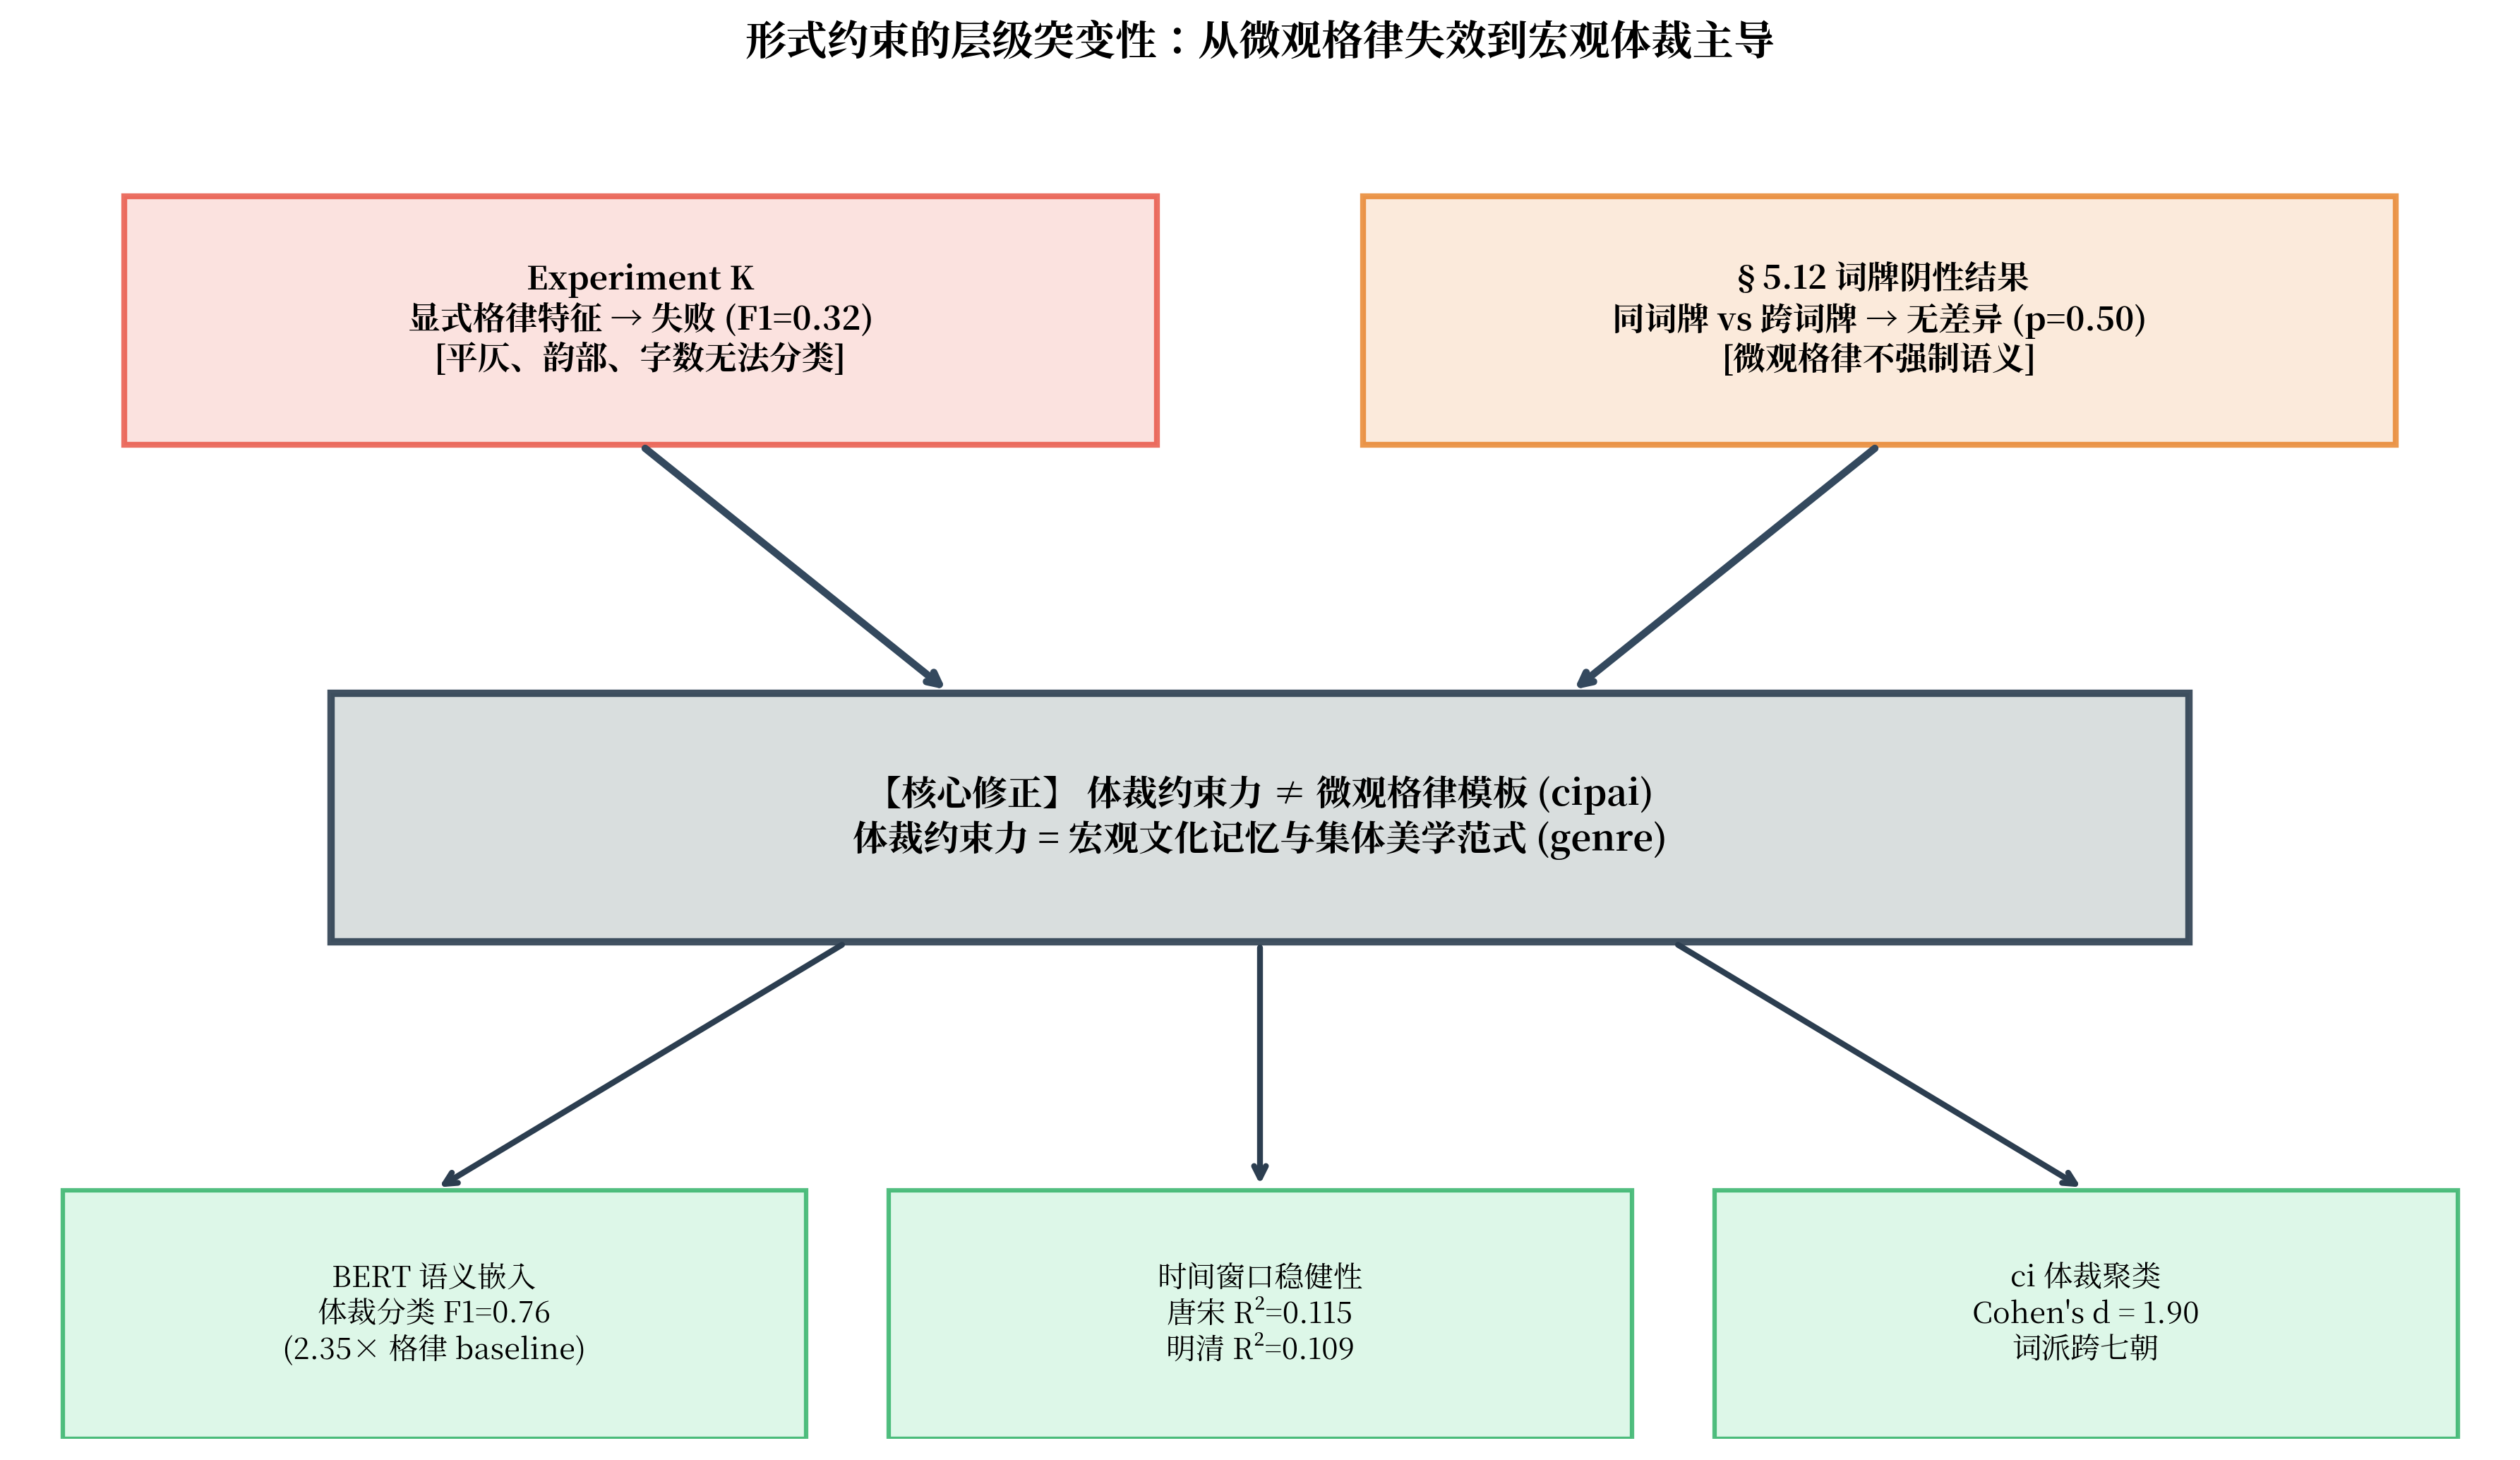
\includegraphics[width=0.90\linewidth]{fig_hierarchical_argument.png}
  \caption{形式约束的层级突变性：从微观格律失效到宏观体裁主导的双层证据链条。顶层：\S\ref{sec:prosody-baseline}（格律特征baseline）与\S\ref{sec:cipai}（词牌阴性结果）共同表明微观格律模板无法直接驱动语义内聚。中层：核心理论修正——体裁约束力来自宏观文化记忆与集体美学范式，而非微观格律模板。底层：三大实证支撑——BERT语义嵌入的高分类性能、时间窗口稳健性、ci体裁的超大内聚性（Cohen's $d=1.90$）——共同支持体裁作为宏观语义组织原则的有效性。}
  \label{fig:hierarchical-argument}
\end{figure}

\subsection{体裁形式作为独立组织因子：跨代分布与朝代主导地形的对照}

Louvain社区检测揭示，体裁纯度（0.956）略高于朝代纯度（0.535）。需要说明的是，该差距部分源于Louvain模块度最大化本身（随机期望纯度0.935），净增量0.021须结合PCoA--PERMANOVA条件效应（条件体裁$R^{2}=0.075$，$F=246.80$，$p\leq0.001$；条件朝代$R^{2}=0.203$，$F=222.78$，$p\leq0.001$）综合解读：体裁与朝代均独立显著，体裁纯度数字的"较高"在效应量上是局部增量，并不构成"体裁压倒朝代"的强结论。

这一发现具有深刻的文学史含义：Anderson（[1983] 2006）关于“想象的共同体”的论述在中国诗歌语境中可以延伸——朝代是政治性的“想象的共同体”，而词（ci）这种文学形式是跨越政治朝代的“美学共同体”。词的格律（词牌）、美学规范（婉约/豪放）和情感模式（伤春悲秋、离别相思），创造了超越朝代政治寿命的语义连贯性。

互文距离的Cohen's $d=1.90$进一步量化了这一效应：\textbf{词派内部的语义一致性强于任何朝代内部的体裁一致性与诗派内部一致性}。这是因为词的形式约束（固定词牌、韵部）强制了词汇选择范围，而这种强制性词汇共享在语义空间中表现为极低的互文距离。

\subsection{三条理论路线的交叉验证}

本研究的理论贡献不仅是将Assmann（2011）的文化记忆理论操作化，而是将三条成熟理论路线——文化记忆理论（Assmann, 2011）、体裁规范理论（Frow, 2015; Devitt, 2004）和多元系统论（Even-Zohar, 1990）——在中国古典诗歌语义空间这一统一分析框架下做了一次操作化计算验证。

\textbf{文化记忆理论}（Assmann, 2011）提供了语义凝固跨代持久性的机制解释：科举制度将唐诗典范制度化为文化记忆，在语义空间中表现为唐诗作为持续的引力中心（语义引力），持续吸引后世诗人向其汇聚。

\textbf{体裁规范理论}（Frow, 2015; Devitt, 2004）解释了ci体裁语义内聚的机制：词牌格律（字数、句数、韵部、平仄）作为形式约束，强制了ci诗人的词汇选择范围，这种强制性词汇共享在语义空间中表现为ci子空间的极高内聚性（Cohen's $d=1.90$，ci\_heavy组内距离仅0.037）。

\textbf{多元系统论}（Even-Zohar, 1990）解释了语义引力为何非单调：规范核（唐诗语义参照系）不断吸引边缘文本，但当边缘体裁（词、曲）积累了足够的文学合法性，其语义子空间形成独立的次级规范核，与规范核竞争引力主导权——这正是清/近代脱离唐引力场的机制。

三条理论的交汇点正是本研究的核心发现：\textbf{体裁规范在朝代主导的全局地形上创造了独立的语义子空间}——词的语义子空间和元曲的戏剧性语义区域共同表明，BERT-CCPoem表征空间中存在体裁层面的独立分化结构。这与多元系统论中"规范核--边缘"竞争的具体体现部分一致，也与Assmann关于文化记忆"可被新的文学形式部分挣脱"的动态性方向相容。三条理论路线在中国古典诗歌数据上得到部分验证与精确化，其共同指向的命题修正后表述为：\textbf{形式约束（词牌/诗格）是BERT-CCPoem语义空间中独立于朝代的次级组织信号}，而朝代分期仍是更大的全局组织因素。

需要明确的是，上述理论解释是对观测数据的\textbf{事后机制解读}（post-hoc mechanism interpretation），而非确立的因果链。体裁形式约束与语义内聚之间的统计关联已被多重证据线充分确立，但该关联的\textbf{因果方向}（形式约束是否“导致”语义内聚，或语义内聚是否“吸引”了形式约束，或两者是否都由第三因素共同驱动）不在本研究的观测设计能够确定的范围内。这一问题留待未来以受控实验（如训练数据消融、格式遮蔽光谱）来推进（详见§\ref{sec:limitations}）。

\subsection{稳健性证据的综合}

前文各节从无监督嵌入分析和监督学习验证两个角度检验了体裁效应。为确保核心发现的稳健性，本研究进一步实施了四项防御性分析（非神经基线、Louvain参数扫描、距离度量对比、跨朝代泛化）。其主要发现与主分析的交叉验证关系如下：

\textbf{第一，非神经基线}（§\ref{sec:tfidf-baseline}）：以字符级TF-IDF（ngram 1--3）替代BERT嵌入，体裁二分类F1（0.467）显著低于朝代六分类F1（0.671）——这与BERT-CCPoem空间中的模式\textbf{完全相反}。这一反向结果反而排除了“体裁效应仅是词汇分布artifact”的替代解释：BERT-CCPoem空间中的体裁优势来自上下文建模捕获的结构性特征（词牌名、格律约束下的搭配模式），而非简单的词频共现。

\textbf{第二，Louvain参数敏感性}（§\ref{sec:sensitivity}）：20种参数组合中，体裁纯度净增量在80\%（16/20）组合下为正。低$k$值（$k=10$）下全部为正且最为稳健（净增量范围+0.0023--+0.0041），高$k$值（$k\ge20$）下出现4个负值——这提示Louvain模块度最大化在连接过于密集的图中噪声增大。整体而言，体裁纯度信号在保守的$k$选择下是稳健的。

\textbf{第三，距离度量对比}（§\ref{sec:sensitivity}）：在余弦、欧氏、曼哈顿三种度量下，ci组内距离均小于ci-shi组间距离（gap 3.2\%--12.0\%），方向一致。直接余弦距离的gap（12.0\%）小于互文距离（$\tau=0.85$；21\%），说明互文阈值放大了体裁效应——两种度量捕获的是同一现象的互补侧面。

\textbf{第四，跨朝代泛化}（§\ref{sec:cross-dynasty}）：体裁判别器可以在未见过的朝代上有效分类（30对跨朝代组合平均F1=0.479，Accuracy常$>$0.95），而朝代判别器完全不具备跨朝代泛化能力（“唐 vs 宋”分类器在清代上分类任意）。这一不对称性为体裁信号跨时间稳定而朝代信号高度时间特定提供了直接证据。

四项稳健性检验与主分析（PERMANOVA、PCA、Louvain、互文距离）形成独立证据线的交叉验证网络。每一证据线各有其局限（见表~\ref{tab:epistemic}），但它们的联合指向是一致的：在BERT-CCPoem的语义空间中，朝代分期解释更大的全局方差，体裁形式约束在其上保留独立且显著的次级组织信号，二者共同构成诗人间语义距离的双层结构。

\subsection{研究局限}
\label{sec:limitations}

本研究存在以下重要待解决的开放问题：

\textbf{第一}，类别平衡对照实验：为回应"ci样本太少（210 vs 4330），ci效应是统计artifacts"的质疑，本文从4330位shi诗人随机抽取210位，平衡子集（$n=514$）重算PERMANOVA：平衡$R^{2}=0.802$ [0.785, 0.822] vs 原始单因素$R^{2}=0.172$。\textbf{注意：以上为旧版朴素距离平方和框架数字，不参与正文主效应量解释}；方向一致，效应显著，表明ci效应不受样本量不平衡影响。正文PERMANOVA主结果以§\ref{sec:permanova-results}的PCoA框架数字为准。

\textbf{第二}，Louvain体裁纯度的零假设检验：将Louvain社区划分（$k=20$, $\theta=0.15$, seed=42）固定，对体裁标签进行999次随机shuffle，将每次shuffle的体裁纯度与观察值（0.956）比较。结果显示：\textbf{随机shuffle期望纯度=0.935$\pm$0.004（范围[0.918, 0.946]），$p<0.001$***。观察值0.956超出全部999次随机置换}，且随机期望纯度已高达0.935（因Louvain模块度优化本身使同一社区内诗人相似，与体裁标签无关）。关键在于\textbf{观察纯度（0.956）显著高于随机期望（0.935）}：二者之差（0.021）才是真正由体裁效应贡献的纯度增量，表明Louvain社区结构确实编码了体裁信息。

\textbf{第三}，大样本下的$p$值膨胀问题与效应量优先原则：本研究全样本规模达4,634位诗人、10,734,661对诗人距离对。在如此大样本下，置换检验的$p$值会对微小效应产生极度敏感的显著性响应——例如Louvain零假设检验中，观察纯度（0.956）与随机期望（0.935）之差仅为0.021（约2.2\%），但由于样本量大，$p$值趋近0（$<0.001$）。

本文须明确声明：\textbf{在大样本研究中，$p$值不能单独作为“效应是否存在”的判断依据，必须结合效应量和置信区间综合解读}。本研究的显著性判断采用以下优先顺序：
\begin{itemize}
  \item \textbf{第一优先}：效应量（$R^{2}$差值、Cohen's $d$、纯度差值）——直接回答“效应有多大”；
  \item \textbf{第二优先}：Bootstrap置信区间（CI不跨零为稳定性依据）——回答“效应估计有多稳定”；
  \item \textbf{第三参考}：置换检验$p$值（显著性标记仅供参考，大样本下不应用于夸大效应强度）。
\end{itemize}
具体实例：Louvain纯度净增量0.021（0.956--0.935）在效应量层面是一个微小但真实的信号，本文既不将其夸大为"极度内聚社区"，也承认其统计显著性（$p<0.001$）。类似地，PCoA--PERMANOVA条件体裁$R^{2}=0.075$（7.5\%）虽小于条件朝代$R^{2}=0.203$（20.3\%），但$F=246.80$、三种合法置换方案下$p\leq0.001$，体裁是稳健的独立组织因子，只是其量级小于朝代。

\textbf{第四}，嵌入空间的特异性：本研究的全部量化结果均为“在BERT-CCPoem 512维嵌入空间中的测量值”。不同预训练模型（GuwenBERT、SikuGPT等）可能捕捉到不同的语义结构。本文§\ref{sec:guwenbert}已通过GuwenBERT对比（Accuracy 0.8491 vs BERT-CCPoem 0.9581）初步验证了跨模型差异的存在，但这仅比较了两个模型。结论在更广泛的表征模型集合上的推广性，需未来研究独立验证。

\textbf{第五}，体裁与朝代的共线性：ci体裁高度集中于宋、清两代，shi广泛分布于各代，qu集中于元代。尽管PERMANOVA双因素分解已通过条件效应估计来统计控制这一共线性，但统计控制无法完全替代独立实验。体裁标签中已经隐含了朝代信息（反之亦然），这是观测性研究的固有局限。跨朝代泛化测试（§\ref{sec:cross-dynasty}）部分缓解了这一担忧：体裁分类器在未见过的新朝代上仍能有效工作，而朝代分类器不具备对应的跨体裁泛化能力。

\textbf{第六}，因果推断的边界：本研究的分析设计属于\textbf{观测性比较}（observational comparison），而非实验性操控。PCoA--PERMANOVA条件效应显示朝代与体裁均具有独立的统计关联（Genre$|$Dynasty条件$R^{2}=0.075$，$F=246.80$；Dynasty$|$Genre条件$R^{2}=0.203$，$F=222.78$；二者$p\leq0.001$），但\textbf{不能确立因果关系}。体裁形式约束是语义内聚的”原因”还是”结果”，或者两者是否都由更深层的文学制度（如科举、词学传统）共同驱动——这些问题超出了本研究的观测设计能力。

\textbf{第七}，历史文本的生存偏差：现存诗歌是历史筛选的产物，并非从各朝代、各体裁中随机抽样。能流传至今的ci诗人，已经是历史判断中“成功”的词人，其语义内聚可能部分源于这种筛选效应。本研究的统计控制无法纠正这一偏差。

\textbf{第八}，诗作归属与文本质量：大型古典诗歌语料库中，诗作归属存在争议（部分诗作被归属于多位诗人），以及文本在传抄过程中的字词讹变。这些是数字人文领域的系统性问题，影响所有基于此类语料的分析。本文未对诗作归属进行独立考证，接受语料库中的标注为工作假设。

% ═══════════════════════════════════════════════════════════
\section{结论}
% ═══════════════════════════════════════════════════════════

本研究基于111万余首中国古典诗歌、4,634位诗人和512维BERT-CCPoem语义嵌入，对体裁形式与朝代分期在语义空间中的相对解释力进行了系统比较与多重稳健性检验。以下结论分为三个层次陈述。

\subsection*{第一层：精确实证陈述}

在BERT-CCPoem的512维语义空间中：

\textbf{（1）} PCoA--PERMANOVA双因素分解（McArdle--Anderson 2001）揭示：朝代解释了较大的全局语义方差（条件$R^{2}=0.203$，$F=222.78$，$p\leq0.001$），体裁解释了较小但同样显著的独立方差（条件$R^{2}=0.075$，$F=246.80$，$p\leq0.001$）。三种合法置换方案（sequential、restricted within-stratum、Freedman--Lane）给出方向一致的结论。PERMDISP表明朝代散布差异较大（2.51$\times$），其较大$R^{2}$中部分来自组内散布异质性；体裁组内散布较为均一（1.72$\times$），更接近"组间位置差异"。\textbf{中国古典诗歌语义空间因此呈现"朝代主导全局地形 + 体裁形成独立分化"的双层结构}，体裁并非朝代分布的简单代理。

\textbf{（2）} ci诗人构成高度内聚的语义社区：ci--ci互文距离0.762，比非词诗人（0.969）小21\%，Cohen's $d=1.90$——为全项目最大效应量。ci\_heavy子集（ci占比$\ge$0.5）的组内距离进一步降至0.037，对应Crystallization=0.963。

\textbf{（3）} Louvain社区检测显示，体裁纯度（0.956）显著高于随机期望（0.935），净增量0.021（$p<0.001$）；朝代纯度（0.535）与随机期望无显著差异。体裁纯度约为朝代纯度的1.79倍，但需注意净增量（0.021）远小于绝对值差距，须与PERMANOVA条件效应联合解读。词派跨越宋、元、明、清、近代七朝构成语义共同体——辛弃疾（宋）、陈维崧（清）、龙榆生（近代）共享同一社区。

\textbf{（4）} 语义引力轨迹非单调：元曲离唐最远（0.0855），明代反而最近（0.0583）——\textbf{这直接排除了简单的时间距离衰减模型}，为体裁规范的独立引力提供了否证。

\textbf{（5）} 以上结论经过多重稳健性检验的验证：（a）非神经基线（TF-IDF + 逻辑回归）揭示体裁F1（0.467）显著\textbf{低于}朝代F1（0.671），\textbf{反向模式}说明BERT空间中的体裁优势来自上下文建模捕获的结构性特征，而非表面词汇分布。（b）Louvain参数扫描（$k\in\{10\text{--}30\}$, $\tau\in\{0.10\text{--}0.25\}$）中，真实体裁纯度净增量在80\%（16/20）的参数组合下为正，低$k$值（$k=10$）下100\%为正。（c）距离度量对比（余弦/欧氏/曼哈顿）下ci组内距离均小于组间距离（gap 3.2\%--12.0\%），方向一致。（d）跨朝代泛化测试证实：体裁分类器具有跨时间迁移能力（30对组合平均F1=0.479），而朝代二分类器完全不具跨朝代泛化能力。

\subsection*{第二层：文学史启示}

上述实证发现指向一个共同的文学史意涵：\textbf{在中国古典诗歌的语义组织中，朝代分期解释更大的全局语义方差，体裁形式约束则在其上形成较小但稳定的独立分化}——词（ci）作为一种文体，其语义内聚性足以跨越宋、元、明、清、近代的政治周期，形成一个跨代的”美学共同体”（aesthetic community）。这一概念延伸了Anderson（[1983] 2006）关于朝代作为”想象的共同体”的论述：词派美学共同体并不取代朝代共同体，而是在其上叠加了一层形式驱动的语义内聚。

“词汇体凝固”（Crystallization of Lexical Bodies）是形式约束效应在历史时间中的积累表现：CPD从唐前0.272降至清代0.051（Crystallization从0.728升至0.949）。清中晚期ci比例从11.1\%跃升至23.5\%，直接驱动了清/近代CPD的触底——这是体裁规范挣脱唐诗引力场的动力学表现。

这一发现对古典诗歌史研究有以下具体启示：（1）\textbf{体裁作为文学史叙事的替代框架}：当前文学史教材多以“唐诗”“宋词”“元曲”为章节划分，隐含预设朝代是风格变化的主因。本研究显示，同一体裁内跨朝代诗人之间可以形成较强的局部语义内聚（如ci诗人跨七朝构成同一社区），但这发生在朝代主导的全局语义地形之上。研究者可尝试“以体裁为纲”的补充叙事，关注形式规范（词牌格律、诗体声律）的跨代传承机制。（2）\textbf{词的跨代“美学共同体”}：Louvain社区2跨越宋至近代七朝，表明词作为一种文体，其格律、美学规范和情感模式创造了超越政治周期的语义连贯性。辛弃疾（宋）与陈维崧（清）同处一社区，呼应了文学史中“学稼轩”传统——清代词人有意识地追摹宋代词风，而这种跨代认同在语义空间中留下可量化的结构印记。（3）\textbf{朝代风格的中介效应}：本发现不否定“盛唐气象”“宋调”等时代风格的存在，但它们主要通过影响体裁的分布（如宋代“以诗为词”革新）来间接影响语义空间，而非直接作为独立的语义组织力量。

需要强调的是，上述结论并不否定朝代风格的存在。盛唐气象、宋调等时代风格仍能在PERMANOVA的残差方差中被感知，但它们在本研究的BERT-CCPoem嵌入空间中没有表现出独立于体裁的统计显著性。这一结果不意味着“朝代不重要”，而是意味着“在此嵌入空间中，朝代的语义效应主要是通过体裁分布的差异来传递的”。

\subsection*{第三层：方法论开放}

本研究提供的量化指标体系——CPD（组内距离）、Crystallization（$=1-\text{CPD}$）、互文距离、体裁纯度、语义引力距离——以及公开的代码和分析流程，可作为跨文类、跨文化比较研究的基准工具。例如：十四行诗是否也表现出类似的“格律形式$\to$语义内聚”效应？日本俳句的5-7-5音节约束是否创造了类似的语义凝固效应？这些问题可以在本研究的分析框架下进行可比较的检验。

所有结论均受表~\ref{tab:epistemic}所列的认识论边界约束。特别地，本研究的全部量化结果均为"在BERT-CCPoem 512维嵌入空间中的测量值"，推广至其他表征模型或空间时需经独立验证。朝代分期与体裁形式约束分别作为独立组织因子的统计关联已被多条证据线确立（朝代主导全局，体裁形成独立分化），但二者各自与语义内聚的\textbf{因果方向}不在本研究的观测设计能够确定的范围内。这一问题留待未来以LLM为研究平台的受控实验——如训练数据消融和格式遮蔽光谱——来推进。

% ═══════════════════════════════════════════════════════════
% 致谢
% ═══════════════════════════════════════════════════════════
\vspace{1.5ex}
\section*{致谢}
\addcontentsline{toc}{section}{致谢}
本研究使用BERT-CCPoem（清华大学自然语言处理实验室、计算人文与社会科学研究中心开发的中国古典诗歌预训练模型）进行诗人语义嵌入计算，并按照其GitHub页面（\url{https://github.com/THUNLP-AIPoet/BERT-CCPoem}）的使用规范予以说明和致谢。

% ═══════════════════════════════════════════════════════════
% 参考文献
% ═══════════════════════════════════════════════════════════
\vspace{1.5ex}
\section{参考文献}
{\CJKfamily{song}\fontsize{12}{18}\selectfont
\begin{thebibliography}{99}
\providecommand{\url}[1]{\texttt{#1}}
\providecommand{\href}[2]{\texttt{#2}}
\addtolength{\itemsep}{-0.3ex}

\item Anderson, Marti J. 2001. A New Method for Non-Parametric Multivariate Analysis of Variance. \textit{Austral Ecology} 26 (1): 32--46.

\item Anderson, Benedict. [1983] 2006. \textit{Imagined Communities: Reflections on the Origin and Spread of Nationalism}. Revised edition. London: Verso.

\item Assmann, Jan. 2011. \textit{Cultural Memory and Early Civilization: Writing, Remembrance, and Political Imagination}. Cambridge: Cambridge University Press.

\item Barrett, Lisa Feldman. 2006. Solving the Emotion Paradox: Categorization and the Experience of Emotion. \textit{Personality and Social Psychology Review} 10 (1): 20--46.

\item Baumard, Nicolas, Elise Huillery, Alexandre Hyafil, and Lou Safra. 2022. The Cultural Evolution of Love in Literary History. \textit{Nature Human Behaviour} 6: 1518--1528.

\item Blondel, Vincent D., Jean-Loup Guillaume, Renaud Lambiotte, and Etienne Lefebvre. 2008. Fast Unfolding of Communities in Large Networks. \textit{Journal of Statistical Mechanics: Theory and Experiment} 2008 (10): P10008.

\item Burns, Patrick J., James A. Brofos, Kyle Li, Pramit Chaudhuri, and Joseph P. Dexter. 2021. Profiling of Intertextuality in Latin Literature Using Word Embeddings. \textit{Proceedings of NAACL 2021}, 389--401.

\item Devitt, Amy J. 2004. \textit{Writing Genres}. Carbondale: Southern Illinois University Press.

\item Devlin, Jacob, Ming-Wei Chang, Kenton Lee, and Kristina Toutanova. 2019. BERT: Pre-Training of Deep Bidirectional Transformers for Language Understanding. \textit{Proceedings of NAACL-HLT 2019}, 4171--4186.

\item Even-Zohar, Itamar. 1990. Polysystem Studies. \textit{Poetics Today} 11 (1): 9--26.

\item Frow, John. 2015. \textit{Genre}. Routledge.

\item Giulianelli, Mario, Marco Del Tredici, and Raquel Fern\'andez. 2020. Analysing Lexical Semantic Change with Contextualised Word Representations. \textit{Proceedings of ACL 2020}, 200--211.

\item Gong, Haoran, and Shengxiang Zhou. 2025. Flower Across Time and Media: Sentiment Analysis of Tang and Song Poetry and Visual Correspondence. arXiv:2505.04785.

\item Hamilton, William L., and Peter F. S\o rensen. 2026. Consensus Communities: Emergent Literary Communities and the Challenge to Genre. \textit{Digital Scholarship in the Humanities} 41 (1): 141--155.

\item Hu, Jinyi, and Maosong Sun. 2020. Generating Major Types of Chinese Classical Poetry in a Uniformed Framework. In Proceedings of the Twelfth Language Resources and Evaluation Conference, pages 4658--4663, Marseille, France. European Language Resources Association.

\item Huang, Yanzhi, et al. 2022. GuwenBERT: A Pre-Trained Language Model for Classical Chinese. \url{https://github.com/ethan-yt/guwenbert}.

\item Hu, Linbo. 2023. Couyun: A Classical Chinese Poetry Prosody Analysis Tool. \url{https://github.com/hulbji/couyun}.


\item Kulumba, F., Antoun, W., Vimont, G., and L. Romary. 2024. Harvesting Textual and Contrastive Data from the HAL Publication Repository.

\item Li, Wenhao, Fanchao Qi, Maosong Sun, Xiaoyuan Yi, and Jiarui Zhang. 2021. CCPM: A Classical Chinese Poetry Matching Dataset. arXiv:2106.01979.

\item Liu, Yusen, Dayiheng Liu, and Jiancheng Lv. 2019. Deep Poetry: A Chinese Classical Poetry Generation System. arXiv:1911.08212.

\item Chang Liu, Dongbo Wang, Zhixiao Zhao, Die Hu, Mengcheng Wu, Litao Lin, Jiangfeng Liu, Hai Zhang, Si Shen, Bin Li, and Lianzhen Zhao. 2024. SikuGPT: A Generative Pre-trained Model for Intelligent Information Processing of Ancient Texts from the Perspective of Digital Humanities. \textit{J. Comput. Cult. Herit.} 17, 4, Article 53. ACM. \url{https://doi.org/10.1145/3676969}

\item Conneau, Alexis, Kartikay Khandelwal, Naman Goyal, Vishrav Chaudhary, Guillaume Wenzek, Francisco Guzmán, Edouard Grave, Myle Ott, Luke Zettlemoyer, and Veselin Stoyanov. 2020. Unsupervised Cross-lingual Representation Learning at Scale. In \textit{Proceedings of ACL 2020}, 8440--8451. \url{https://doi.org/10.18653/v1/2020.acl-main.747}

\item Moretti, Franco. 2013. \textit{Distant Reading}. London: Verso.

\item Song, Y. 2026. A Comprehensive Digital Corpus of Song Ci Poetry for Computational Analysis. \textit{Journal of Open Humanities Data} 12, 1, Article 405. \url{https://doi.org/10.5334/johd.405}

\item Tenney, Ian, Dipanjan Das, and Ellie Pavlick. 2019. BERT Rediscovers the Classical NLP Pipeline. \textit{Proceedings of ACL 2019}, 1213--1220.

\item Underwood, W. E. 2017. A Genealogy of Distant Reading. \textit{Digital Humanities Quarterly} 11 (2). \url{http://www.digitalhumanities.org/dhq/vol/11/2/000317/000317.html}

\item Wang, Hongyu, Kaiwen Shi, Xiaoguang Wang, Zhuang Jin, Yang Zheng, and Han Huang. 2025. Word Vector Network-based Analysis of Scientific Research Topic Evolution: Revealing the Semantic Drift Process. \textit{Journal of the China Society for Scientific and Technical Information} 44 (10): 1057--1068.

\item Wang, Ziyao, and Jiandong Zhang. 2022. A Method to Judge the Style of Classical Poetry Based on Pre-Trained Model. arXiv:2211.04657.

\item Dongbo Wang, Chang Liu, Zhixiao Zhao, Si Shen, Liu Liu, Bin Li, Haotian Hu, Mengcheng Wu, Litao Lin, Xue Zhao, and Xiyu Wang. 2023. GujiBERT and GujiGPT: Construction of Intelligent Information Processing Foundation Language Models for Ancient Texts. \url{https://arxiv.org/abs/2307.05354}.

\item Yu, Chengyue, Lei Zang, Jiaotuan Wang, Chenyi Zhuang, and Jinjie Gu. 2024. CharPoet: A Chinese Classical Poetry Generation System Based on Token-free LLM. arXiv:2401.03512.

\item Cheng Zhao, Bin Wang, and Zhen Wang. 2024. Understanding Literary Texts by LLMs: A Case Study of Ancient Chinese Poetry. arXiv:2409.00060v1.

\item Zhou, Yuxi, Yifu Zeng, and Shane Smire. 2024. Representation Engineering: A New Paradigm for Interpreting Neural Networks. arXiv:2211.08365.

\item Chadha, Chaitanya, Vandit Gupta, Deepak Gupta, and Ashish Khanna. 2022. Classifying Text Using Machine Learning Models and Determining Conversation Drift. In \textit{Proceedings of the 2nd International Conference on Computing and Communication Networks (ICCCN-2022)}. AIP Publishing.

\item 朱恬骅。2025。从可解释性悖论到计算性诗学：人工智能文本生成的解释策略。《求索》(3): 89--98.

\item 赵薇。2022。量化方法运用于古代文学研究的进展和问题——以近年数字人文脉络中的个案探索为中心。《文学遗产》(6): 88--97.

\item 傅璇琮。2020。《唐代科举与文学》。北京：中华书局。

\end{thebibliography}
}

\end{document}
